\documentclass[10pt]{book}

\usepackage{graphicx}
\graphicspath{{./Images/}}

\usepackage{multirow}

% ? 
\usepackage{caption}
\usepackage{subcaption}

%Remove ugly green and red boxes. 
%\usepackage[hidelinks]{hyperref}

%appendix
%\usepackage[toc,page]{appendix}

%Feyn
\usepackage{feynmp-auto}
\usepackage{scalerel}
\newcommand{\mylbrace}[2]{\vspace{#2pt}\hspace{6pt}\scaleleftright[\dimexpr5pt+#1\dimexpr0.06pt]{\lbrace}{\rule[\dimexpr2pt-#1\dimexpr0.5pt]{-4pt}{#1pt}}{.}}
\newcommand{\myrbrace}[2]{\vspace{#2pt}\scaleleftright[\dimexpr5pt+#1\dimexpr0.06pt]{.}{\rule[\dimexpr2pt-#1\dimexpr0.5pt]{-4pt}{#1pt}}{\rbrace}\hspace{6pt}}

\newcommand{\quark}[9]{
  \fmfcmd{ %input TEX; input latexmp; setupLaTeXMP(packages="amssymb,amsmath");
    style_def quark#1 expr p =
    pair a, b, m, n;
    if (substring (0,4) of "#6" = "left") or (substring (1,5) of "#6" = "left"):
      a = point 0 of p; b = point length(p) of p + (#7); m = point length(p) of p + (#8);
      path q; q = a{m-a}..tension ypart(#4)..{right}b;
      label.lft(btex #2 etex, point xpart(#3) of q shifted (#5))
    fi;
    if (substring (0,5) of "#6" = "right") or (substring (1,6) of "#6" = "right"):
      a = point 0 of p + (#7); b = point length(p) of p; m = point 0 of p + (#8);
      path q; q = a{right}..tension ypart(#4)..{b-m}b;
      label.rt(btex #2 etex, point ypart(#3) of q shifted (#5))
    fi;
    cdraw subpath (#3) of q                          shifted (#5);
    if substring (0,1) of "#6" = "-":
      cfill (tarrow (reverse(q),(xpart(#3)+ypart(#3))*0.46*xpart(#4))) shifted (#5);
    else:
      cfill (tarrow (q,(xpart(#3)+ypart(#3))*0.46*xpart(#4))) shifted (#5);
    fi;
    enddef;}
  \fmf{quark#1,tension=0}{#9}}


\begin{filecontents*}{vovalblob.mp}
	vardef vovalblob (expr bd, a) (text vl)=
	forsuffixes $=vl:
	if not vexists $: venter $; fi
	vlist[vlookup $]decor.shape := fullcircle xscaled a;
	vlist[vlookup $]decor.size := bd;
	vlist[vlookup $]decor.sty := "shaded";
	endfor
	enddef;
\end{filecontents*}

\def\fmfovalblob#1#2#3{\fmfcmd{input vovalblob; vovalblob ((#1), (#2), \fmfpfx{#3});}}

\DeclareMathSymbol{\comma}{\mathpunct}{letters}{"3B}

%Standard thesis size
\usepackage[a4paper,left=3cm,right=2.5cm,top=3cm,bottom=3cm,]{geometry}

%To make [H] Work
\usepackage{float}

%Loading comment package 
\usepackage{comment}

% for fancy looking tables
\usepackage{booktabs} 

%This package slashe
\usepackage{slashed}

% Good old Checkmarks
\usepackage{pifont}

%Mathematical expressions 
\usepackage{amsmath}
\usepackage{amssymb}

% inputs 
\usepackage[utf8]{inputenc}
\usepackage[english]{babel}

%Using Sub files
%\usepackage{subfiles}

%Horizontal line
%\usepackage{cancel}

\usepackage{tabularx}

%using a colored text 
\usepackage[dvipsnames]{xcolor}

\usepackage[normalem]{ulem}





%%% Commands 
%\DeclareUnicodeCharacter{2009}{\,} 

\newcommand{\ro}[1]{\textrm{#1}}
\newcommand{\U}[1]{\mathrm{U}(1)_{\mathrm{#1}}}
\newcommand{\Z}[1]{\mathrm{Z}(1)_{\mathrm{#1}}}
\newcommand{\SU}[1]{\mathrm{SU}(2)_{\mathrm{#1}}}

\renewcommand{\(}{\left(}

\renewcommand{\)}{\right)}

\renewcommand{\[}{\left[}

\renewcommand{\]}{\right]}

\newcommand{\del}{\partial}

%check marks
\newcommand{\cmark}{{\color{green}\ding{51}}}%
\newcommand{\xmark}{{\color{red}\ding{55}}}%

%% ?? 

\usepackage[final,fis]{uaThesisTemplate}
\setlength\extrarowheight{2pt}

\def\topfigrule{\kern 7.8pt \hrule width\textwidth\kern -8.2pt\relax}
\def\dblfigrule{\kern 7.8pt \hrule width\textwidth\kern -8.2pt\relax}
\def\botfigrule{\kern -7.8pt \hrule width\textwidth\kern 8.2pt\relax}

\usepackage{titlesec}
\newcommand{\sectionbreak}{\clearpage}

\def\ThesisYear{2021}

% ? 
% \usepackage{flexisym}

%% Doc Start!
\begin{document}


\TitlePage
  \HEADER{\BAR\FIG{
\includegraphics[height=60mm]{uaLogoNew.pdf}}} 
%	
  {\ThesisYear}
  \TITLE{João Pedro \\ Dias Rodrigues }
        {Análise fenomenológica em teorias para lá do Modelo Padrão: os casos do B-L-SM mínimo e de um 3HDM do tipo BGL \\ \ \\ Phenomenological analysis in beyond the Standard Model theories: the cases of the minimal B-L-SM and of a BGL-like 3HDM}
\EndTitlePage
\titlepage\ \endtitlepage % empty page

\TitlePage
  %\HEADER{\BAR}
  \HEADER{\BAR}{\ThesisYear}
  \TITLE{João Pedro \\ Dias Rodrigues }
        {Análise fenomenológica em teorias para lá do Modelo Padrão: os casos do B-L-SM mínimo e de um 3HDM do tipo BGL \\ \ \\ Phenomenological analysis in beyond the Standard Model theories: the cases of the minimal B-L-SM and of a BGL-like 3HDM}
  \vspace*{15mm}
  \TEXT{}
       {Dissertação apresentada à Universidade de Aveiro para cumprimento dos requisitos necessários à obtenção do grau de Mestre em Engenharia Física, realizada sob a orientação científica do Doutor António Morais, Investigador Doutorado do Departamento de Física da Universidade de Aveiro e sob a coorientação do Doutor Roman Pasechnik, Professor Associado do Departamento de Astronomia e Física Teórica da Universidade de Lund.}
    \vfill 
	\begin{center}
		%\vspace{5.5cm}
		\hspace{-2cm}
		\TEXT{}
		{O trabalho nesta tese foi suportado pelo projeto \textit{From Higgs Phenomenology to the Unification of Fundamental Interactions} com referência PTDC/FIS-PAR/31000/2017.}
		\begin{figure*}[h]
			\hspace{7.3cm}
			\includegraphics[width=0.57\textwidth]{logos.pdf}
		\end{figure*}
	\end{center}
\EndTitlePage
\titlepage\ \endtitlepage % empty page

\TitlePage
  \vspace*{55mm}
  \TEXT{\textbf{o j\'uri~/~the jury\newline}}
       {}
  \TEXT{presidente}
       {\textbf{António Cunha}\newline {\small
        Professora Associado do Departamento de Física da Universidade de Aveiro}}
  \vspace*{5mm}
  \TEXT{vogais}
       {\textbf{António Morais}\newline {\small Investigador de nível inicial do Departamento de Física da Universidade de Aveiro}}
  \vspace*{5mm}
  \TEXT{}
       {\textbf{Nuno Castro}\newline {\small
        Professor auxiliar da University of Minho. }}
  \vspace*{5mm}
  \TEXT{}
  {\textbf{Roman Pasechnik}\newline {\small
  		Professor associado da University de Lund. }}
  \vspace*{5mm}
\EndTitlePage
\titlepage\ \endtitlepage % empty page

\TitlePage
  \vspace*{55mm}
  \TEXT{\textbf{agradecimentos~/\newline acknowledgements}}
       {Eu gostaria de expressar os meus mais profundos agradecimentos ao meu orientador, Professor António Morais, que me guiou e encorajou a ser profissional e a fazer as escolhas certas. Sem a sua ajuda e paciência o projeto não teria sido realizado.  
       \\ \ \\ 
       Ao Roman queria agradecer as oportunidades dadas, destacando, em particular, o tempo e acompanhamento que disponibilizou na minha visita a Lund.
       \\ \ \\ 
       Ao João Pino eu queria do fundo do meu coração agradecer todos os conselhos e apoio que me levaram a ter sucesso neste trabalho. A tua perseverança e ética de trabalho são inspiradoras.
       \\  \ \\ 
       Ao Felipe, que, apesar de de ter chegado tão tarde, teve sempre uma presença apreciada graças ao seu impecável sentido de humor e sabedoria. 
       \\  \ \\ 
       Finalmente, um especial obrigado à minha familia por todo amor e apoio que motivou a por fim a esta etapa da minha vida. \\   
       \ \\ \ \\ }
  \TEXT{}
       {I wish to express my sincere appreciation to my supervisor, Professor António Morais, he convincingly guided and encouraged me to be professional and do the right thing.  Without his persistent help and endless patience, this project would not have been accomplished.
       \\ \ \\ 
       To Roman, I would like to thank you for the opportunities given emphasizing, in particular the trip to Lund where you gave me so much of your time and availability.
       \\ \ \\ 
       Pino, I whole-heartedly appreciate the advice given. It proved monumentally helpful for the success of this thesis. Your perseverance and work ethic are, with no exaggeration, inspiring.
       \\ \ \\ 
       To Felipe,  who's presence, although having joined us so late into the project, was always welcome thanks to his impeccable sense of humour and down to earth wisdom.
       \\ \ \\ 
       Last but not least, I wish to acknowledge the support and love given by my family and friends, who kept me going. This work would not have been possible without their input.
        }
\EndTitlePage
\titlepage\ \endtitlepage % empty page

\TitlePage
  \vspace*{55mm}
  \TEXT{\textbf{Resumo}}
       {O Modelo Padrão (MP) é neste momento o protótipo de análise em de física de partículas. 
       	%
       	Este une numa estrutura auto consistente e bem motivada, três das quatro forças fundamentais do universo. 
       	%
       	No entanto, é do consenso geral que o MP não seja uma teoria completa. 
       	%
       	Pese embora o excelente acordo entre muitas das suas previsões e medições experimentais, a existência de observações fenomenológicas e de questões conceptuais sem explicação no MP, segue a necessidade de física nova. 
       	\\ \ \\ 
       	Neste sentido, a comunidade cientifica tem propostos diversos modelos motivados pela procura de respostas a estas questões, bem como na tentativa de incorporar observáveis tais como a massa de neutrinos ou a existência de matéria escura matéria escura.
       	\\ \ \\ 
       	Estes modelos conseguem abordar diferentes problemas do MP tipicamente através da introdução de novas partículas ou interações. 
       	%
       	Contudo, as suas previsões devem ser consistentes com a realidade. 
       	%
       	Neste trabalho procurámos verificar a viabilidade fenomenológica de dois modelos tais como, por um lado, uma extensão minimal ao MP com uma simetria B-L e, por outro, uma extensão ao setor de Higgs com dois adicionais dobletos.
       	\\ \ \\
       	O foco deste trabalho foi o desenvolvimento de um conjunto de rotinas com a capacidade de, independentemente do modelo, simular as previsões teóricas e confrontá-las com os mais recentes limites experimentais.
       	%
       	Foi também estudando o impacto que dos diversos constrangimentos experimentais na previsão de nova física para ambos os modelos.
       	\\ \ \\                                                                                                                                                                                                                                                                                                                                                                
       	Neste trabalho, começámos por uma breve revisão ao MP. Seguidamente, foram introduzimos os dois modelos de nova física para além do modelo padrão, começando com os aspetos teóricos necessários para a interpretação dos resultados numéricos alcançados. Finalizámos com uma apresentação de possíveis sinais de nova física que cada cenário poderá oferecer e concluímos.
       }
\EndTitlePage
\titlepage\ \endtitlepage % empty page

\TitlePage
  \vspace*{55mm}
  \TEXT{\textbf{Abstract}}
       {%
       At this time the Standard Model (SM) of particle physics is the propotype for the analysis of particles and their interactions. 
       %
       It unifies three out of the four known fundamental forces of the universe in a well motivated framework, however the current consensus among physicists is that it is incomplete theory. 
       %
       This, unfortunatly, comes despite the general agreement between the SM predictions and some experimental messurements. 
       %
       Alas, given modern phenomenological questions which the SM cannot awnser, there is now the necessity for new physics.  
       \\ \ \\ 
       Motivated by this and the desire to include new observables, such as neutrino masses and dark matter the cientific comunity has proposed a wide range of new models. 
       \\ \ \\ 
       These models can adress several different problems present in the SM trough the adition of new particles and interactions. 
       % 
       However, these models must all be constricted by experimental bounds. 
       %
       In this thesis we verify the fenomenological viability of two such models, being one the Baryon minus Lepton minimal extension of the SM, and the other a Higgs sector extension of the SM with two additional doublets. 
       %
       \\ \ \\ 
       %
       The focus of this work was the creation of a set of routines that would allow us to analyze particle intearction independent of model with ease. 
       %
       We also investigate the impact of a number of experimental constraints and examine the new physics predictions made by each model. 
       %
       \\ \ \\ 
       %
       This work begins with a general review of the Standard Model as it is the foundation for the remaining theories we present.
       %
       Following this, we introduce the remaning two theories entitled beyond the standard model kicking off with the required theoritical background as to be able to properly discuss our results. 
       %
       We finalize with a discussion on what each scenario could represent in the way of new physics and conclude. 
       % 
       %B-L-SM and the 3HDM. Both these theories will be first introduced theoretically and then checked against the latest constraints trough our numerical scans. We finalize each section by present the results of this numerical analysis. 
       }
\EndTitlePage
\titlepage\ \endtitlepage % empty page

\pagenumbering{roman}
\tableofcontents

\cleardoublepage
\listoffigures

\cleardoublepage
\listoftables

\cleardoublepage

\pagenumbering{arabic}
\setcounter{page}{1}

%\chapter{Introduction}
%\label{ch:Intro}

\newpage
% 

\renewcommand{\cleardoublepage}{}
\renewcommand{\clearpage}{}

\chapter{Introduction}
\label{Chap:Introduction}

Our current understanding of all subatomic phenomena must be based on the Standard Model (SM) of particle physics. 
%
The SM has thus far been the best description for the experimentally observed particles and their interactions at the electroweak (EW) scale. 
%
In 2012 a resonance was discovered at the Large Hadron Collider (LHC) that confirmed the existence of its last predicted particle, the Higgs boson, revealing, at last, the existence of the Higgs mechanism \cite{collaborations2016measurements}. 

The development of the SM was an arduous task, leading scientists to successfully combine three of the four fundamental interactions of nature, the electromagnetic, weak and strong interactions, in a well motivated framework. 

However, despite its successes, the SM still lacks a strong explanation for several experimental observations. 
%
%They have become more numerous by the decade and to provide a "short" overview of some of them. 
%
%To enumerate some of these previously alluded too problems, we have:
%
First, the SM can not explain for one of the most important, the existence of dark matter \cite{Bergstr_m_2000}. 
%
%This is a fundamental flaw since the SM lacks a possible dark matter candidate, or dark particle. % {\color{red} (It is already discussed in 6. Should I put the ciation here again?).} 
%
%Secondly, neither the SM, nor the theory of general relativity, offer any justification for the existence of baryon asymmetry in the universe, i.e. why is the universe primarily made of matter rather than anti-matter \cite{book_Baryion}. 
%
Second, the SM does not offer any justification for the existence of a baryon asymmetry in the universe, i.e. why is the observable universe primarily composed of matter rather than anti-matter \cite{book_Baryion}. 
%
%Note, that a popular proposed scenario as to explain cosmic baryon asymmetry is the Electroweak baryogenesis (EWBG) which requires some sort of new physics (NP) structure \cite{Morrissey2012}. 
%
Third, the SM suffers from peculiar oddities in the fermion sector in the form of unjustified mass and mixing hierarchies. 
%
This is usually referred to as the flavor problem. % and is considered a sizable drawback of the SM. 
%
As an example, we observe the top quark mass ($\mathcal{O}(100)$ GeV) to be five order of magnitudes heavier than the up quark ($\mathcal{O}(1)$ MeV), and eleven orders of magnitude above the highest neutrino mass limit ($\mathcal{O}(0.1)$ eV) set by kinetic beta decay analysis \cite{Mertens_2016}.
%
%{ ( \color{red} Ask Morais: Eu sei que existem experiencias de oscilações mas eu acho que só havia um higher limits de massa nos neutrinos. Basicamente eu não sei se dizer massas de neutrinos é correto. ) }
%
These high differences are thought to be too large to be natural, so a physical property that could justify such gap is a common motivation of many Beyond the Standard Model (BSM) frameworks. 
%
Fourth, neutrino masses (as alluded to) are not predicted by the SM. 
%
Their existence was discovered after the observation of neutrino oscillations \cite{PhysRevD.89.013001}. 

In addition to these, there are still many other subtle flaws, such as emerging flavor and $g-2$ anomalies. 
% like the lack of a strong phase transition, the $R_{\kappa}$ parameter and $g-2$ anomaly of lepton magnetic moments, etc. 
%
%These are just some of the typical justifications given to explore possible BSM scenarios. 
%
%The holy grail of which would be a model that solves all these problems in a properly motivated framework that addresses these and many more cosmological and phenomenological problems and is in harmony with all measurements.  

While the literature is rich in BSM models, narrowing down the scope of such theories through phenomenological analysis is a very worthwhile endeavor. This work will be a review of two such studies. % We try to present one of these studies in this work. % to the steady advancement of a more complete theory. 

The typical procedure consists in performing large a numerical scans on the parameter space. %  analysis of all possible combinations of free parameters of a given model, which we call the parameter space, as to narrow it down trough compassion with modern bounds set by experiments. 
%
This allows us to assess the model's viability and whether it can explain observed deviations. 
%
% predict exactly what observations this model could still allow for in experimental detection and measure if the proposed model could have a significant impact as to explain observed deviations or if it is, in a extreme case, completely excluded by modern limits.   
%
% and see how much phenomenology it can explain, or not, and even perhaps exclude the model under modern collider experiments.
%
%Paradoxically, as of late these studies have become progressively harder to perform regardless of the improvement in hardware given that the available space for NP gets reduced by each successful particle experiment. 
%
Experiments such as the the ATLAS and CMS collaborations at the LHC, have been posing stringent bounds on popular BSM scenarios. 
%
As the available space for new physics decreases, it becomes more challenging to agree with observations without falling within the possibility of fine tuning our model parameters.
%
%Fine tuning consists in carefully balancing several contributions as to, cancel or magnify as to be allowed by current bounds.    

%{\color{blue} How to properly explain what fine tunning is? Should I?}
%
%Note, that the SM has shown itself consistence with most constraints that were initial believed to be a possible gateway to NP i.e. divergences from its predictions. Thus, the search continues for hints at possible directions to complete the SM. One of these is brought to use trough flavor physics, as we'll soon examine further on. 

Conventionally, phenomenological simulations of BSM scenarios in these multi-dimensional parameter spaces have been made in large computer-clusters requiring several weeks of computational time trough conventional Monte-Carlo methods, which are the basis for the work presented in this thesis.
%
% Move to conclusions
%although some modern studies have incorporated new strategies to scan these complex problems like machine learning. Similar to done by our colleagues in \cite{freitas2020phenomenology}. These new methods promise to greatly increase the efficacy of similar studies.  
%
%Although this is the basis of the work presented here a effort was made to incorporate new machine learning routines via the initial building of smaller learning sets by conventional methods. 
%
%Unfortunately this wasn't accomplished in this work due to the expectational setbacks. A feature of this year, that affected partially the quality of the work. 

%%%% so far so good

%During this thesis we embark in a small expedition into two possible BSM scenarios.
%Bellow replaced 
In this thesis we start with a short review of the SM. Then, we present and discuss the minimal Baryon-Lepton number symmetry extended SM (B-L-SM), as well as a three Higgs Doublet Model (3HDM) supplemented with a BGL-like global symmetry. 

%Over the course of this thesis we intent to perform two of these BSM studies. However we must begin by laying down the fundamental basis for this type discussion by presenting a short overview of the SM. 
%
%In this thesis we will embark in two of these kind of BSM studies.  
%
%Start by laying down the fundamental basis for this BSM discussion by presenting a short overview of the SM followed by a discussion into potential extensions of this framework.
%Afterwords we will present, first the B-L-SM (Baryon-Lepton-SM) model, a simple unitary extension of the SM - and then, move on to a more complex model with additional Higgs doublets fields as an attempt to present a framework that addresses the flavor problem via the Three Higgs Doublet Model (3HDM) with a stabilizing symmetry.
%
%We will see how each of these models addresses specific problems differently and discuss the advantages and disadvantages of a simple unitary extension versus a multiple doublet approach. 

While models with multiple Higgs doublets can easily offer an explanation for the observed excess of charge parity or $\mathcal{CP}$, violation, they often suffer from the possible presence of tree-level Flavour Changing Neutral Currents (FCNCs). 
%
These FCNCs are undesirable \cite{ILYUSHIN2020114921}, at least in large number, given current experimental bounds, typically requiring additional mechanisms to suppress their existence. 

%Examples of such supression mechanisms exist for a wide range of models, such as seen in \cite{Huitu2019} for a model containing a Unitary extension. 

% mechanisms have to be put in place to prevent them, while in the case of the simple unitary extensions such problems tend to not arise . 

We also want to stress that, while the minimal structure of the Higgs sector postulated by the SM is not an immediate contradiction to experimental measurements it is not manifestly required by the data. 
%
In fact, an extended scalar sector is often desirable feature of BSM scenarios despite the tight bounds of Higgs boson couplings to the SM gauge bosons and heavy fermions \cite{10.1093/ptep/ptaa104}. 
%{\color{red} Ask:Morais How do I cite q exactly instead of the whole corpus}.   

%These additions are partially motivated by the fact that in the SM, the single Higgs doublet is a bit "overstretched" in the SM.
%
%It  takes  care,  simultaneously of the gauge boson masses, up and down-type quarks masses and leptons masses. 
%
%N-Higgs-doublet models have multiple scalar and complex fields that can relax this, while the simpler unitary additions cannot address this observation % {\color{red} Is it true? Couldn't we have a singlet generate the top quark masses or only the third generation, do I need a citation?}.   
%
%In fact these multiple Higgs doublet models are often engineered based on a naturalness argument, that is,  the  notion  of  generations  can  be  brought  to  the  Higgs  sector and these might help explain mass hierarchies. % This is not the particular case of the model we will present in this thesis. 

%Both these extensions have the bonus of leading to remarkably rich  phenomenology (for a detailed review, see e.g. Refs. ( \cite{branco1999cp,Branco_2012,Ivanov_2017} ). And in general BSM scenarios offer features  as  several  Higgs  bosons,  charged  and neutral, modification of the SM-like Higgs couplings, FCNC at tree level, additional forms of CP-violation from the scalar sector, and opportunities for cosmology such as scalar DM candidates and modification of the phase transitions in early Universe. {\color{blue} Repeated, Fix later.} Also, many BSM models including supersymmetry (SUSY), gauge unification models, and even string theory constructions naturally lead to several Higgs doublets at the electroweak scale.

%We give a higher repute to the Higgs Sector since fermion masses and mixing patterns relate often to the specific structure of the Higgs sector. Also, the addition of new scalars offer a large playground for collider experimentation and often offer the inclusion of new neutrino physics. 

%In short two particular multi-Higgs models will be presented in this work a phenomenological study of a 3 Higgs Doublet model (3HDM) with softly broken $\U \times \mathrm{Z_2}$ symmetry and a simple Unitarity, $\mathrm{U(1)}$, extension of the SM based on the apparent Baryon minus Lepton symmetry (B-L-SM). We'll investigate what can be learned from these models and what other physical experiments constrict them. 

%The SM extensions featuring non-minimal Higgs sectors with extra Higgs doublets in analogy to fermion generations in the SM provide a fruitful playground for constructing successful BSM scenarios (for a detailed review, see e.g. Refs. \cite{branco1999cp,Branco_2012,Ivanov_2017} ).

%There is also no constraints stemming from the $\rho$ parameter here.  Since all doublets couple to the gauge-bosons in the same way, the W and Z masses are determined by the single value, the sum of real VEVs. Assuming this value is 246 GeV it would retain the condition $\rho = 1 $ at tree-level. 

%Multi-doublet models offer novel opportunities for CP-violation.  Within the SM, it is put by hand coming entirely from the Yukawa matrices which must be complex.  In multi-doublet models, a relative phase between vevs can arise just as a result of the minimization of the potential. Leading to a more natural and spontaneous CP-violation. 

%A real or even complex singlet extension is a also simple pathway to extending the SM. In a generic model with a SM Higgs Doublet the addition of a generic gauge singlet scalar, S, could prove a link between the SM fields and a unknown hidden sector. 
%
%In spite of our ignorance of this hidden sector, we can simply assume a generic renormalizable self-interaction for the scalar S and investigate the joint $(\phi,S)$ potential. This would lead to a generic mixing, $\alpha$ between scalars. 

%In the case the additional scalar field is complex this brings a additional degree of freedom and has the possibility of 3 neutral scalars mixing, depending on the shape of the VEV. Producing  a slightly  richer  collider  phenomenology  and  complicating its analysis.  

%Are heavily constricted from experimental measurements we know that in this framework fermions and gauge bosons should primary couple to $h_\phi$. This type of mixing suppression, ($\alpha < 10^3$), but even so the heavy Higgs can in most cases decay into a pair of light ones if this channel is open kinematically, providing a avenue for detection. 

%On the other hand, one or both new scalars can be symmetry protected against decay, yielding simple models of one or two-component dark matter or models with one DM candidate and a strong electroweak phase transition.

%Before moving on, let us make a remark on the (absence of) CP-violation in the singlet extension of SM. Although the potential contains many complex coefficients, it does not produce CP-violating effects in the scalar sector, see \cite{branco1999cp}.

\chapter{The Standard Model of Particle Physics}
\label{Chap:SM}

%\section{The Standard Model of Particle Physics}
%
%To pave the way for our future studies we present the SM. Complete with a overview of it's mechanisms and a brief historical introduction.
%
%\section{Motivation}

% { \color{red} Note! The motivation should explain why we are going indepth into flavour, and the Yukawa sector. There has to be a purpose to this section! } 

As stated in chapter \ref{Chap:Introduction}, it is hard to question the validity of the SM as a successful, at least approximate, framework, with whom to describe the phenomenology of particle physics up to the largest energy scales probed by collider measurements so far, although some inconsistencies remain and must be addressed.  
%
Note, what we call the SM is the conjugation of several theories, quantum chromodynamics (QCD), Higgs sector and the EW theory. 
%
% The last piece, the EW theory, was introduced in the nineteen sixties by Glashow, Salam and Weinberg \cite{SALAM1964168}, since then it has been extensively tested both in contemporary direct searches for new physics and indirect probes via e.g. flavour anomalies a\cite{Gr_newald_2008}. It awarded the authors the 1979 Noble prize of physics \cite{NobelPrize:2009-Physics}.  
%
%B. %, { \color{gray} and as said, it's been consistent with most to date.} 

The formulation of the SM came from previous principles relating to symmetries in nature, specifically symmetry in physical laws. 
%
In fact, much in modern physics can be attributed to Emmy Noether's work. She deduced, trough her first theorem, that if the action in a system is invariant under some group of transformations (symmetry), then there exist one or more conserved quantities (constants of motion) \cite{doi:10.1080/00411457108231446}. 

Physicists took this idea and were led to a fundamental question, is it possible that upon imposing to a given Lagrangian the invariance under a certain group of symmetries to reach a given form for its the dynamics? 
%
%These dynamics would be in our context, particle interactions. This train of thought first led to Quantum Electrodynamics (QED), then Quantum Chromodynamics (QCD) and finally the SM. 
%
We can quote Salam and Ward in Ref \cite{Salam1961}: % A. Salam and J. C. Ward, Nuovo Cim.19, 165 (1961). 

\textit{“Our basic postulate is that it should be possible to generate strong,  weak and electromagnetic  interaction terms (with all their correct symmetry properties and also with clues regarding their relative strengths) by making local gauge transformations on the kinetic energy terms in the free Lagrangian for all particles.”} % { \color{red} Question Morais: Is this really relevant I like it but it might be excess }

Although we are glossing over a lot of complexity in this statement, given that for the SM to be properly formulated, additional concepts are required. 
%
As in the case of weak interactions, the presence of a massive weak gauge boson requires the concept of spontaneous breakdown of the gauge symmetry via what is known as the Higgs mechanism \cite{higgs1964broken}. 
%
While the concept of asymptotic freedom played a crucial role in describing perturbatively the strong interaction at short distances \cite{politzer1973reliable}.  

\section{Internal symmetry of the Standard Model}
%
The SM is a gauge Quantum Field Theory (QFT), that is, manifestly invariant under a set of field transformations. The SM gauge group \cite{Quigg:1983gw}, $\mathcal{G}_{SM}$,% is seen in Eq. \ref{eq:SM_Group} . 
%
%The SM is manifestly invariant under of a set of field transformations. The SM is a gauge group \cite{Quigg:1983gw}, $\mathcal{G}_{SM}$, is seen in, 
%
\begin{equation}
\mathcal{G}_{SM} = \mathrm{SU}(3)_{\mathrm{C}} \times \SU{L} \times \U{Y}   .
\label{eq:SM_Group}
\end{equation} 
%
Where, $\mathrm{SU}(3)_{\mathrm{C}}$, with $\mathrm{C}$ being colour, is the group that describes the QCD sector, responsible for the strong force. This symmetry will remain unbroken by the EW Vacuum Expectation Value (VEV).
%
Secondly, we have the $\SU{L} \times \U{Y}$ portion, with L being Left and Y the hypercharge, that will be broken by the Higgs mechanism into $\U{Q}$, the electromagnetic gauge symmetry.

Each particle in the SM stems from a field that is charged in a particular manner on each of these groups.  
%
Recall that Quantum Field Theory (QFT) treats particles as excited states of their respective quantum fields, which are more fundamental than the particles. 
%
Interactions between particles are described by interaction terms in the Lagrangian involving their corresponding quantum fields.
%
Of which each interaction can be visually represented by a Feynman diagram according to perturbation theory.
%
Generally speaking, an interacting QFT can not be solved analytically, requiring the use of perturbative methods. 
%
In this mindset, one employs the use of Feynman diagrams to better visualize interactions at any given order in perturbation theory.

It is important to highlight that given the invariance under the group in Eq.\,(\ref{eq:SM_Group}), it is impossible for any field, besides the scalar field, to have an explicit mass term in the bare Lagrangian.
%
In this chapter we shall present how the mass of particles is generated via the Higgs mechanism.
%
And offer a brief discussion of flavor physics in the SM and how flavor changing currents can point to NP. 

%{ \color{gray} All masses for the fermions and leptons are generated trough their interactions with the Higgs Boson. This mass generation as the Higgs Boson settles into it's VEV is called the Higgs Mechanism. } 

\subsubsection{Particle States and Fields}

The particle spectrum of the SM is composed by, the gauge bosons, $W^\pm$ and $Z$ bosons, mediators of the weak interactions, the photon $\gamma$, the electromagnetic interaction messenger and the strong force mediators, the gluons, $G$. 
%
Additionally, the model is also composed  by the matter particles, the fermions, composed by quarks and leptons. A spin-0 scalar also emerges known as the Higgs Boson, $h$. 

Leptons and quarks are organized in three generations each, with 2 pairs by each generation leading to 6 different particles. 
%
For quarks we have the up and down for the first generation, charm and strange for the second as well as the top and bottom for the third one. 
%
Similarly, there are 6 types of leptons, the 3 charged leptons, electron, muon and tau, and the associated neutrinos. 
%
These are represented in different manners, being that the quarks are represented by $(u,d,c,s,t,b)$ while leptons as $(e,\nu_{e},\mu,\nu_{\mu},\tau,\nu_{\tau})$, where $\nu$ denotes the neutrinos. 

%Fermions are half integer spin particles where half of which have electrical charge (except the neutrinos).  
%
While quarks interact via the weak, electromagnetic and strong forces, the charged leptons only feel the electromagnetic and weak forces and the neutrinos are weakly interacting.  
%
A physical fermion is composed of a left-handed and a right-handed field. The left-handed components of the fermions are doublets under $\mathrm{SU(2)}_L$, 
%
\begin{equation}
L^i= \begin{pmatrix}
\nu_{e_L} \\ e_L 
\end{pmatrix},
\begin{pmatrix}
\nu_{\mu_L} \\ \mu_L 
\end{pmatrix},
\begin{pmatrix}
\nu_{\tau_L} \\ \tau_L 
\end{pmatrix} 
\quad 
\text{and} \quad Q^i= \begin{pmatrix}
u_{L} \\
d_L 
\end{pmatrix},\begin{pmatrix}
c_{L} \\
s_L 
\end{pmatrix}
,\begin{pmatrix}
t_{L} \\
b_L 
\end{pmatrix} ,
\end{equation}
%
where the $i$ index stands for generation, often designed as the flavour index. Conversely the right-handed components are singlets of  $\SU{L}$ and are represented as,
%
 \begin{equation}
e^i_R=\{e_R,\mu_R,\tau_R\}, \quad  u^i_R=\{u_R,c_R,t_R\}, \quad d^i_R=\{d_{R},s_{R},b_{R}\} . 
\end{equation}
%
Note also that the quarks form triplets of $\mathrm{SU(3)_C}$ whereas leptons are color singlets, meaning that only quarks interact strongly. 
%
The Higgs boson also emerges from an $\mathrm{SU(2)_L}$ doublet with the form,
%
\begin{equation}
H=\begin{pmatrix}
\phi^1 + \; i \; \phi^2 \\
\phi^3 + \; i \; \phi^4  
\end{pmatrix} \equiv \begin{pmatrix}
\phi^+ \\
\phi^0 
\end{pmatrix}, 
\end{equation}
%
%The Lagrangian that describes all vector particles and gauge fields in the SM can be writen as
%
where we see the four components that correspond to the respective degrees of freedom of the Higgs Field.
% 
After the process of Spontaneous Symmetry Breaking (SSB) of the $\mathrm{SU(2)_L} \times \U{Y}$ group, the charges read as,
%
\begin{table}[H]
\caption{Quark and Lepton charges}
\centering
\begin{tabular}{ccc}
  \hline & $\mathrm{SU(3)_C}$ & $\mathrm{U(1)_Q}$ \\
  \hline 
Up type quarks $(u,c,t)$ & \textbf{3} & 2/3 \\
Down type quarks $(d,s,b)$ & \textbf{3} & -1/3 \\
Charged leptons $(e,\mu,\tau)$ & \textbf{1} & -1 \\
Neutrinos  $(\nu_e,\nu_\mu,\nu_\tau)$  & \textbf{1} & 0 \\
  \hline	
\end{tabular}
\end{table}


\subsubsection{Gauge Group Numbers}

The full set of SM fields and respective quantum numbers are are shown in the tables \ref{table1} and \ref{table2}. These show us the representations of these fields, e.g. if a field $F$ has a quantum number of 3 under $\mathrm{SU(2)_L}$ then he would be a triplet of of $\mathrm{SU(2)_L}$, \ $F^a = (F^1,F^2,F^3)$, where $a$ is an index in the adjoint representation of the group.   
%
\begin{table}[H]
\centering
\caption{Gauge and Scalar fields in the SM}
\label{table1}
\begin{tabular}{@{}cccccc@{}}
  \hline	
 Fields & Spin 0 field & Spin 1 Field & $ \mathrm{ SU(3)_C \times SU(2)_L \times U(1)_Y } $  \\
  \hline	
 Gluons  & $\times$  & $G^a$ & (\textbf{8},\textbf{1},0) \\	
A bosons & $\times$  & $A^a$ & (\textbf{1},\textbf{3},0)   \\
B bosons & $\times$  & $B$   & (\textbf{1},\textbf{1},0)   \\
Higgs field & ($\phi^\pm, \phi^0 )$  & $\times$ & (\textbf{1},\textbf{2},1) \\ \hline
\end{tabular}
\end{table}
%
The gauge groups presented in table \ref{table1} are composed of 12 generators and are governed by the following algebra, 
% 
\begin{equation}
\left[ M_a , M_b \right] = i f_{abc} M_c \quad \left[ T_a , T_b \right ] = i \epsilon_{abc} T_c \quad \left[ M_a , T_b \right] = \left[ M_a , Y \right] = \left[ T_b,Y \right] = 0  \ , 
\end{equation}
%
where for $\mathrm{SU(3)_c}$, $M_a = {\lambda_a}/{2}$ , with $(a = 1, . . . , 8)$. As for $\mathrm{SU(2)_L}$, we have $T_i= \sigma_i/{2} $, $(i = 1, 2, 3)$, and for $Y$ is the generator of $U(1)_Y$. The symbols $\lambda_a$ and $\sigma_i$ represent the Gell-Mann and Pauli matrices respectively. 
%
\begin{table}[H]
\centering
\caption{Fermion fields in the SM}
\label{table2}
\begin{tabular}{@{}cccccc@{}}
  \hline	
 Fields & Spin $\frac{1}{2}$ Field & $\mathrm{ SU(3)_C \times SU(2)_L \times U(1)_Y} $   \\
  \hline	
Quarks (3 gen.) & $Q=(u_L,d_L)$ & $(\mathbf{3},\mathbf{2},{1}/{3})$ \\	
$\quad$        & $u_R$ & $(\mathbf{3},\mathbf{1},{4}/{3})$   \\
$\quad$   & $d_R$ & $(\mathbf{3},\mathbf{1}, -{2}/{3})$   \\
Leptons (3 gen.) & $L=(\nu_{e_L}, e_L )$ & $(\mathbf{1},\mathbf{2},-1)$  \\
$\quad$   & $e_R$ & $(\mathbf{1},\mathbf{1},-2)   $ \\ \hline
%
\end{tabular}
\end{table}
%
From here, given the gauge group in, Eq.\,(\ref{eq:SM_Group}) and accounting for the charges and fields, we can derive the form of the SM's Lagrangian. 



%\subsection{Fields, Particles and Lagrangian of the SM}

\subsubsection{Lagrangian Formulation }
%
Given the SM gauge groups seen in  Eq.\,(\ref{eq:SM_Group}), the charges seen in Tables \ref{table1} and \ref{table2} and their algebra, the covariant derivative, $D_\mu$, can be shown to read as, 
%
\begin{equation}
\label{eq:PartialDefSM}
D_\mu = \partial_\mu - i g_s M^a G^a_\mu - i g T^i A^i_\mu - \frac{1}{2} i g' Y B_\mu \quad ,  
\end{equation}  
%
We can expect 3 different type of couplings, $g_s$ related to the $\mathrm{SU(3)_C}$ subgroup, $g$ to the $\mathrm{SU(2)_L}$ and $g^\prime$ to $\mathrm{U(1)_Y}$. The associated canonical field strength tensors would be,
\begin{align}
G_a^{\mu \nu} & = \partial^\mu G^\nu_a - \partial G^\mu_a - g_s f_{abc} G_a^\mu G_b^\nu ,  \\ 
A_a^{\mu \nu} & = \partial^\mu A^\nu_a - \partial^\nu A^\mu_a  - g  \epsilon_{abc} A^\mu_b A^\nu_c , \\
B^{\mu \nu}   & = \partial^\mu B^\nu - \partial^\nu B^\mu .
\end{align}
%
Given these we can now present the SM Lagrangian. It is often convenient to do so in portions, usually divided in three \footnote{There is also the need for the introduction of gauge fixing terms and ghosts. However, this is merely a formal requirement and does not imply addition of new physical states.} sections,
\begin{equation}
\mathcal{L}_{SM} = \mathcal{L}_{kin}  +  \mathcal{L}_{Yuk} +  \mathcal{L}_{\phi} , 
\end{equation}
Where we have the kinetic portion of the SM terms, $\mathcal{L}_{kin}$, responsible for  free propagation of particles, the Yukawa portion, $\mathcal{L}_{Yuk}$,  corresponding to interactions of particles with the Higgs Boson, and finally the $\mathcal{L}_{\phi}$ scalar potential. The full kinetic portion of the SM read, 
%
\begin{align}
\label{eq:KinSM}
\mathcal{L}_{kin} = & - \frac{1}{4} G^{\mu \nu}_a G_{a \, \mu \nu}  - \frac{1}{4}  A^{\mu \nu}_a A_{a \,\mu \nu}  
- \frac{1}{4}  B^{\mu \nu} B_{\mu \nu} \nonumber \\ 
 & -i \bar{Q}_{L_i} \slashed{D} Q_{L_i} 
   -i \bar{u}_{R_i} \slashed{D} u_{R_i}  
   -i \bar{d}_{R_i} \slashed{D} d_{R_i}  
   -i \bar{L}_{L_i} \slashed{D} L_{L_i}    
   -i \bar{e}_{R_i} \slashed{D} e_{R_i}   \\
 & - (D_\mu H)^\dagger ( D^\mu H ) ,  \nonumber 
\end{align}
where $\slashed{D}$ is the Dirac covariant derivative, $\gamma^\mu D_\mu$ where $\gamma^\mu$ being the gamma matrices. 
%
From the last line of Eq.\,(\ref{eq:KinSM}) and with Eq.\,(\ref{eq:PartialDefSM}) we will present how the fields $A^a_\mu$ and $B_\mu$ give rise to the weakly interacting vector bosons $W^\pm$ and $Z^0$ and the electromagnetic vector boson $\gamma$. Contrary to the colour sector, where the eight generators $G^a_\mu$ simply correspond to eight gluons $G$ mediating the strong interactions.
%
The scalar potential part is written as, 
%
\begin{equation}
\label{eq:PotentialSM}
\mathcal{L}_{\phi} = -\mu^2 H H^\dagger - \lambda (H H^\dagger)^2 .
\end{equation}
%
Finally the Yukawa portion of the Lagrangian is, 
%
\begin{equation}
\label{eq:YukawaSM}
\mathcal{L}_{Yuk} = Y^u_{ij} \bar{Q}_{L_i} u_{R_j}  \tilde{H} + Y^d_{ij} \bar{Q}_{L_i}  d_{R_j} H  + Y^e_ij \bar{L}_{L_i}  e_{R_i} H + \text{H.c.} \ ,
\end{equation}
%
where, $\tilde{H}=i\sigma_2 H$ and H.c. stands for Hermitian conjugate, also the terms $Y^{e,u,d}$ stands for the Yukawa matrices, these are generic $3\times3$ with complex and adimensional matrix elements. Note that all indices seen in Eqs.\,(\ref{eq:KinSM}), (\ref{eq:PotentialSM}) and (\ref{eq:YukawaSM}), ($j,i$) are summed over. 

%{ \color{red} Perguntar ao Morais : Remover o italico dos campos? } 
%
%{ \color{gray} It is due to the Yukawa interactions between the Higgs and the fermions and leptons that these acquire their masses once the Higgs settles into his VEV. } { \color{blue} same as before }
%
%We'll define these fields in the relevant section. Note that naturally all indices seem in Eqs. \ref{eq:KinSM} \ref{eq:PotentialSM} and \ref{eq:YukawaSM}, ($j,i$) are summed over. 


\renewcommand{\cleardoublepage}{}
\renewcommand{\clearpage}{}

\section{The Higgs Mechanism and the Mass Generation of the Gauge Bosons}

From what was defined above, we can now study the process SSB by which, 
%
\begin{equation}
\SU{L}\times\U{Y} \rightarrow \U{Q}. 
\end{equation} 
%
Enabling us to find the real physical states of the gauge bosons and the origin of their mass. Let us consider the part of the Lagrangian containing the scalar covariant derivatives, the scalar potential and the gauge-kinetic terms:
%
\begin{equation}
\mathcal{L}_{Gauge} \supset (D_\mu H)(D^\mu H)^\dagger - \mu^2 H^\dagger H - \lambda (H^\dagger H)^2 - \frac{1}{4}  W^{\mu \nu}_a W_{a \,\mu \nu}  
- \frac{1}{4}  B^{\mu \nu} B_{\mu \nu} \ . 
\label{eq:GaugeSM}
\end{equation} 
% 
We expect a phase shift to occur, namely one that ensures $\mu^2 < 0$ while at the same ensuring that the field now explicitly breaks the $\mathrm{SU(2)_L \times U(1)_Y}$. For this to happen we expect the shifted squared value of the Higgs field to be,
%
\begin{equation}
(H^\dagger H)^2 = \frac{-\mu^2}{2\lambda} \equiv  v^2  , 
\end{equation} 
called the EW-Vacuum expectation value (EW-VEV), its value is experimentally measured to be $v \approx 246$ GeV. 
%
The choice of vacuum can be aligned in such a way that we have,
\begin{equation}
H_{min} = \frac{1}{\sqrt{2}} \begin{pmatrix} 0 \\
v 
\end{pmatrix}  .
\end{equation}

Given that now the $\mathrm{SU}(2)_{\mathrm{L}} \times \mathrm{U}(1)_{\mathrm{Y}}$ symmetry is broken down to $U(1)_{\mathrm{Q}}$ we jump from a scenario where there were four generators, which are $T^{1,2,3}$ and $Y$, to, after the breaking, having solely one unbroken combination that is $Q =  (T^3 + Y/2)$ associated to the electric charge.
%
This means that in total we will have three broken generators, thus, from the Goldstone theorem, there would have to be created three massless particles. % { \color{red} Do I need citation? }

These Goldstones modes however can be parameterized as phases in field space and can be absorbed into the physical basis fields, leaving us with a single physical massive scalar, the Higgs boson. 
%
Note that, with this transformation we are removing three scalar degrees of freedom and transferring them to the gauge bosons.  %However, they cannot just disappear from the theory and will be absorbed by the massive gauge bosons.
%
%In fact, a massless gauge boson contains only two scalar degrees of freedom (transverse and polarization). Meanwhile, a massive vector boson has two transverse and a longitudinal polarization, i.e., three scalar degrees of freedom. 
%
So, while before the breaking of the EW symmetry we have four massless gauge bosons, after the breaking we are left with three massive ones.
%
%This means that there are three extra scalar degrees of freedom showing up in the gauge sector.
%
%It is then commonly said that the goldstone bosons are ``eaten" by the massive gauge bosons and the total number of scalar degrees of freedom in the theory is preserved. 
%
Therefore, without loss of generality, we can rewrite the Higgs doublet as
%
\begin{equation}
 \begin{pmatrix}
\phi_1 + i \phi_2 \\ 
v + h + i \phi_3 
\end{pmatrix} = H  \rightarrow H =  \frac{1}{\sqrt{2}} \begin{pmatrix}
0 \\ 
v + h 
\end{pmatrix}  .
\label{shame}
\end{equation}
Once the Higgs doublet shifts to the EW-VEV, the Lagrangian (\ref{eq:GaugeSM}) can be recast as:
%
\begin{align}
\mathcal{L}^\prime = & \frac{1}{2} \partial_\mu h \partial^\mu h - \frac{1}{2} (2v^2 \lambda) h^2
 - \frac{1}{4}  W^{\mu \nu}_a W_{a \, \mu \nu}  
- \frac{1}{4}  B^{\mu \nu} B_{\mu \nu}  \nonumber \\
& + \frac{1}{8} v^2 g^2 (A^1_\mu A^{1,\mu}+ A^2_\mu A^{2,\mu}) +  \frac{1}{8} v^2  (g^2  A^3_\mu A^{3,\mu} + g^{\prime 2} B_\mu B^\mu - 2 g^2 g^{\prime 2} A^3_\mu B^\mu )  \ , 
\label{complicatedpart}
\end{align}
%
A few things become obvious. First, we have a lot of mass terms stemming from the squared gauge fields and a lonesome mass term belonging to the real scalar field we know to be the Higgs field. This makes the Higgs boson mass to be given by,
%
\begin{equation}
M_h= (2v^2 \lambda).  
\end{equation}
%
To obtain masses for the gauge bosons we need to rotate the gauge fields to a basis where the mass terms are diagonal. First, it is straightforward to see that the electrically charged eigenstates are given by %\ref{gagestate}
%First the fields that carry defined charge that can be easily shown to be 
\begin{equation}
W^\pm_\mu = \frac{1}{\sqrt{2}} (A^{1}_\mu \pm i A^{2}_\mu) , 
\label{gagestate}
\end{equation}
meaning that the mass of the W bosons is, 
\begin{equation}
M_{W^\pm}= \frac{1}{2} v g .
\end{equation}
%
The situation becomes a bit more complicated for the second term in (\ref{complicatedpart}) due to a mixing between $A_\mu^3$ and $B_\mu$. In the gauge eigenbasis the mass terms read
%
\begin{equation}
\begin{pmatrix}
A_\mu^3 && B_\mu
\end{pmatrix} \cdot  \frac{1}{2} v^2 \begin{pmatrix}
g^2  & -g g^\prime \\
-g g^\prime & g^{\prime 2} 
\end{pmatrix} \cdot \begin{pmatrix}
A^{\mu,3} \\  B^\mu
\end{pmatrix}  , 
\end{equation} 
%
which can be diagonalized to obtain,
%
\begin{equation}
\begin{pmatrix}
A_\mu && Z_\mu 
\end{pmatrix} \begin{pmatrix}
0  & 0 \\
0  & \frac{1}{2} v \sqrt{g^2 + g^{\prime 2}} 
\end{pmatrix}  \begin{pmatrix}
A^\mu \\ Z^\mu
\end{pmatrix} , 
\end{equation}
%Where the new eigenvectors that represent the $Z$ boson and the photon, $A^\mu$ in terms of the former base are written as,
%
we identify the eigenvector associated with the null eigenvalue to be the photon and the massive one, $ M_Z =  \frac{1}{2} v \sqrt{g^2 + g^{\prime 2}} $, to be the Z boson. Such eigenvectors can be written as
%
\begin{align}
A_\mu &=\cos(\theta_W) B_\mu + \sin(\theta_W) A_\mu^3 ,  \\  
Z_\mu & =- \sin(\theta_W) B_\mu + \cos(\theta_W) A_\mu^3 , 
\end{align}
%
where $\theta_W$ is the so called Weinberg mixing angle and is defined as, 
%
\begin{equation}
\cos(\theta_W)=\frac{g}{ \sqrt{g^2 + g^{\prime 2}}} . 
\end{equation}
%
%{ \color{gray} Thus showing the massless photon along with a massive Z boson with mass $M_Z= \frac{1}{2} v \sqrt{g^2 + g^{\prime 2}} $ }. 
%
So we conclude our exploration of the electroweak sector with all the correct massive spectrum observed and its origin discussed.

\section{Fermion Masses in the Standard Model and Quark Mixing}
\label{Chap_1_Sec_3}

As referenced previously, given the charges of the fermion and lepton fields we cannot construct a gauge invariant theory with explicit mass terms for fermions. 
%
The mass of these particles are generated through the Higgs mechanism, via Yukawa terms between the fermions and the scalar field. 
%
These interactions can be seen in Eq\,(\ref{eq:Yukawa2}), 
%
\begin{equation} 
\label{eq:Yukawa2}
\mathcal{L}_{Yuk} = Y^u_{ij} \bar{Q}_{L_i} u_{R_j}  \tilde{H} + Y^d_{ij} \bar{Q}_{L_i}  d_{R_j} H  + Y^e_{ij} \bar{L}_{L_i}  e_{R_i} H + \text{H.c.} , 
\end{equation} 
%
as the Higgs field settles into the EW VEV (see Eq.\,(\ref{shame})) mass terms for the quarks and leptons are generated. 
%
The Higgs mechanism generates the mass for all the fermionic and leptonic particles except for neutrinos, this is due to the SM not containing right handed neutrinos, i.e it is impossible build terms that would lead to neutrino masses without explicitly breaking the SM symmetry group.
% 
The addition of right handed neutrino fields is very commonly made in BSM scenarios. 

To reach the physical states from the weak eigenbasis we must diagonalize the Yukawa matrices. This is done through bi-unitary transformations. 
% 
We can write these transformation under the form,
%
\begin{equation}
\label{YukawaMasses} 
M^{u,d,e}_{\text{diag.}}= U^{u,d}_L Y^{u,d} U^{u,d}_R \frac{v}{\sqrt{2}} , 
\end{equation} 
%
where $U^{u,d}_L$ and $U^{u,d}_R$ are the required 4 unitary matrices. 

%{\color{gray} The charged lepton Yukawa matrix can always be made real and positive through a bi-unitarity transformation.  
%
%Meaning the Yukawa matrix for the leptons contains only 3 real physical parameters that correspond to the Lepton masses. } 
%
For simplicity sake we assume that the leptonic Yukawa couplings matrix $Y^{e}$ is flavour diagonal i.e. a diagonal matrix needing not to be transformed. This makes only the quarks to be relevant to our discussion.  

Naturally, we can invert Eq.\,(\ref{YukawaMasses}), returning, 
\begin{equation}
\label{eq:YukawaBiUni}
%\begin{split}
Y^u_{ij} = \frac{\sqrt{2}}{v} (U_L^u M^u_{\text{diag.}} U_R^u)_{ij} \quad , \quad Y^d_{ij} = \frac{\sqrt{2}}{v} (U_L^d M^d_{\text{diag.}} U_R^d)_{ij} . 
%\end{split}
\end{equation}
%
Considering the Higgs mechanism, we can see this change creates mass terms for physical quark fields by replacing the result of Eq.\,(\ref{eq:YukawaBiUni}) in the Yukawa portion of the Lagrangian (Eq.\,(\ref{eq:YukawaSM})).
%
\begin{gather}
\mathcal{L}_{Yuk} \supset 
- \frac{v}{\sqrt{2}} Y^d_{ij} \begin{pmatrix} \overline{u}_{L\,i} & \overline{d}_{L\,i}  \end{pmatrix}  d_{R\,j} \tilde{H}
%
-\frac{v}{\sqrt{2}} Y^u_{ij} \begin{pmatrix} \overline{u}_{L\,i} & \overline{d}_{L\,i}  \end{pmatrix} \, u_{R\,j} + \text{H.c.} \nonumber  \\ 
% % % 
 \Downarrow \nonumber \\
-(U_L^d M^d_{\text{diag.}} U_R^d)_{ij} d_{L\,i} \, d_{R\,j}  - (U_L^u M^u_{\text{diag.}} U_R^u)_{ij} u_{L\,i} \, u_{R\,j} + \big(\text{Interactions with } h\big) + \text{H.c.} \\ 
 \Downarrow  \nonumber \\ 
-M^d_{\text{diag.}_j} d_{L\,i}^\prime \, d_{R\,j}^\prime  - M^u_{\text{diag.}_j} u_{L\,i}^\prime \, u_{R\,j}^\prime + \big(\text{Interactions with }h\big) + \text{H.c.}  \nonumber  
\end{gather}
%
where the primed fields are the quark fields in the mass basis, defined as, 
\begin{equation}
\begin{split}
d^\prime_{L,R} = U^d_{L,R} d_{L,R}, \\
u^\prime_{L,R} = U^u_{L,R} u_{L,R}. 
\end{split}  
\end{equation}
% 
Note that the increasing masses seen in each generation depend directly on the  hierarchy of the Yukawa terms. This means that the mass of all particles directly relates to how strongly they each interact with the Higgs boson.
%
If you then take into account the real masses e.g. for the leptons, the tau mass is in the GeV range while the electron's is in the 0.1 MeV range. This translate to very different couplings for each flavour. 
%
This hierarchy is unjustified in the SM. 

As a result of this redefinition we can now look at the gauge interactions to see that charged currents appear where $W^\pm$ couples to the physical $u^\prime_{L_j}$ and $d^\prime_{L_j}$ quarks. 
%
The coupling of the fermions to the gauge fields changes by virtue of the fact that only left handed quarks are $\mathrm{SU(2)_L}$ doublets. If we expand the up and down quark fields on the kinetic portion of the Lagrangian,
%
\begin{equation}
\label{LagFermFCCCs}
\begin{aligned}
\mathcal{L}_{ferm} \supset & 
\frac{1}{2} \bar{u}^\prime_L \gamma^\mu \left( g^\prime Y B_\mu + g Z_\mu  \right) \left(U^u_L U^{u \dagger}_L \right) u^\prime_L - \frac{1}{\sqrt{2}} g \bar{u}^\prime_L \gamma^\mu \left( U^u_L U^{d \dagger}_L \right) d^\prime_L W^+_\mu \\    
- 
& \frac{1}{\sqrt{2}} g \bar{d}^\prime_L \gamma^\mu \left( U^u_L U^{d \dagger}_L \right) u^\prime_L W^-_\mu 
+ 
\frac{1}{2} \bar{d}^\prime_L \gamma^\mu \left( g^\prime Y B_\mu - g Z_\mu \right) \left( U^d_L U^{d \dagger}_L \right) d^\prime_L \quad , 
\end{aligned}
\end{equation}
%
By employing properties of unitary matrices, namely, $ \mathrm{U}^{u,d}_{L,R} \mathrm{U}^{u,d \dagger}_{L,R} = 1$, we note that the interactions with the neutral bosons remain the same in the mass basis.
%
However the charged currents are affected by this change.
%
Therefore, we define the Cabibbo-Kobayashi-Maskawa (CKM) matrix, as $V_{CKM} = U^u_L U^{u ^\dagger }_R $ and write the sensitive terms,
%
\begin{equation}
\mathcal{L}_{kin} \supset \frac{1}{\sqrt{2}} g \overline{u}^\prime_L \gamma^\mu V_{CKM} d_L^\prime W^+_\mu + \text{H.c.} \quad , 
\end{equation}
%
The CKM matrix, is a $3 \times 3$ unitary matrix. It is a parametrization of the three mixing angles and a CP-violating KM (Kobayashi-Maskawa) phase. % There are many possible conventions to represent the CKM matrix.
%
The mixing angles refer to those between the up and down quark families. We can see their hierarchy in Fig. \ref{fig:QuarkCKM}.

It is through this complex phase in the CKM matrix that the SM can account for the phenomena of $\mathcal{CP}$ violation.
%
First observed in the famous $K^0$ decay into $\mu^+$ $\mu^-$ ($CP=+1$ and $CP=-1$ respectively) \cite{PhysRevLett.13.138}, that won the 1980 Nobel Prize \cite{NobelPrize:1980-Physics}. 
%
The discovery opened the door to questions still at the core of particle physics and of cosmology today.
%
Not just the lack of an exact CP-symmetry, but also the fact that it is so close to a symmetry.

\begin{figure}[H]
	\centering
	\vspace{1em}
   \begin{fmffile}{feyngraph_box}
   \begin{fmfgraph*}(175,60)
   \fmfstraight
   \fmfleft{i2,K,i1}
   \fmfright{o2,o1}
%    % quarks
   \fmf{fermion}{i1,t1}
    \fmf{fermion}{t4,i2}
    \fmflabel{d}{i1}
    \fmflabel{$\overline{\text{s}}$}{i2}
    \fmfv{l.d=65,l.a=180,l={$\text{K}^0$\mylbrace{76}{0}}}{K}
    % placeholders quarks-muons
    \fmf{phantom,tension=1}{t1,t2}
    \fmf{phantom,tension=1}{t4,t3}
%    % muons
    \fmf{fermion,tension=1}{t2,o1}
    \fmf{fermion,tension=1}{o2,t3}
    \fmflabel{$\mu^-$}{o1}
    \fmflabel{$\mu^+$}{o2}
%    % box loop
    \fmf{boson,tension=0,label=$\text{W}^-$,label.side=left}{t1,t2}
    \fmf{boson,tension=0,label=$\text{W}^+$,label.side=left}{t3,t4}
    \fmf{fermion,tension=0,label=u}{t1,t4}
    \fmf{fermion,tension=0,label=$\nu_\mu$}{t3,t2}
    \fmfv{d.shape=circle,d.size=4,l=$\sin(\theta_{\mathrm{C}})\quad$,l.a=110}{t1}
    \fmfv{d.shape=circle,d.size=4,l=$\cos(\theta_{\mathrm{C}})\quad$,l.a=-110}{t4}
    \fmfv{d.shape=circle,d.size=4}{t1}
    \fmfv{d.shape=circle,d.size=4}{t4}
    \end{fmfgraph*}
    \end{fmffile}
\vspace{1em}
	\caption{Box diagram describing $K_L^0\rightarrow\mu^-\mu^+$, through an intermediate $u$ quark. }
	\label{fig:Kaon}
\end{figure}
%
We avoided discussing leptons since in the SM their mass eigenstates can be easily shown to have no real consequence besides a change of basis. 
%
We might also note a very interesting feature of the Standard Model, by consequence of the $\mathrm{SU(2)_L \times U(1)_Y }$ symmetry we can see that in Eq.(\ref{LagFermFCCCs}) there are no interactions of the right handed unitary matrices and thus no mixing, coupling, or charged currents of right handed quarks, making them theoretically invisible. % to measurements.  
%
The nature of CKM elements and how the quarks behavior differs when interacting weakly trough neutral currents can be seen in the following figure,
%
\begin{figure}[H]
	\centering
	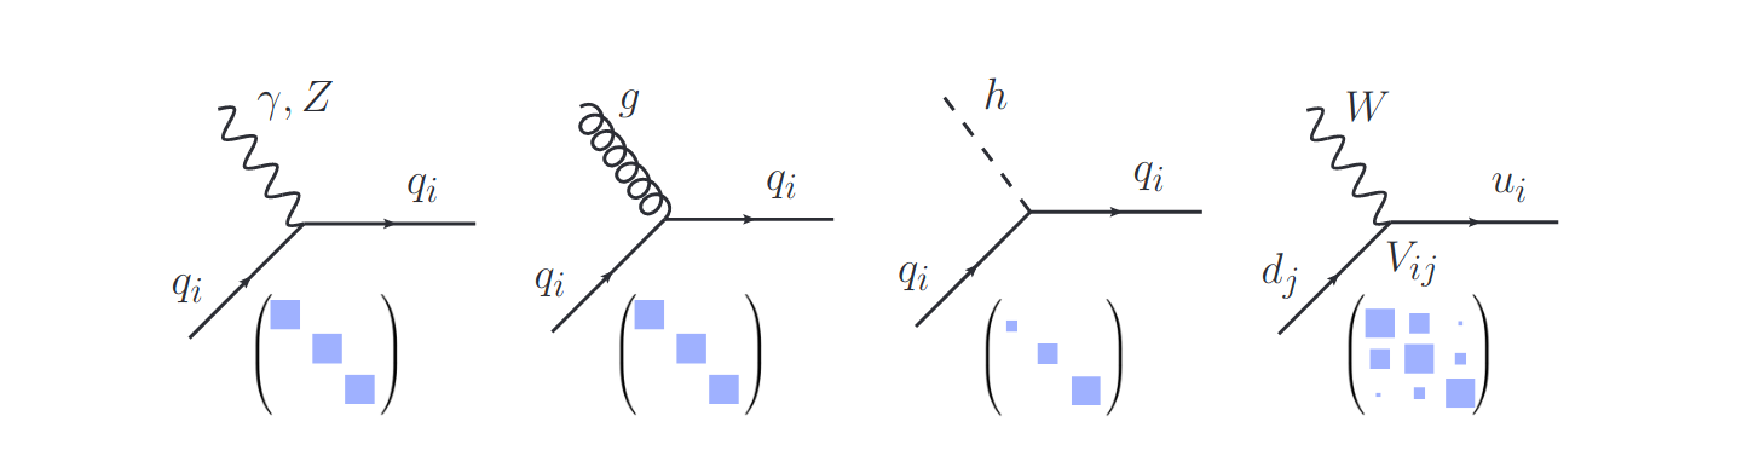
\includegraphics[width=0.9\textwidth]{TestYukawaCouplings.pdf}
	\caption{Feynman diagrams for flavour conserving couplings of quarks to photon, $Z$ boson, gluon and the Higgs (the first three diagrams), and the flavour changing coupling to the $W$ (the last diagram). The $3\times3$ matrices are visual representations of couplings in the generation space, with couplings to $\gamma$ ,$Z$, $g$ being flavour universal, while the couplings to the Higgs are flavour diagonal but not universal. Finally the couplings involving the $W$ are flavour changing and hierarchical.}
	\label{fig:QuarkCKM}
\end{figure}
%´
Note, the CKM matrix elements are fundamental parameters of the particle physics and their precise determination a important landmark for experimental particle physics. It follows then that reproducing the quark mixing parameters is fundamental for BSM searches that include changes to how the quarks interact with possible new Higgs bosons. 

\subsection{Charged Flavour Currents vs. Neutral Flavor Currents}

It is very noteworthy to highlight a important distinction between flavor changing neutral and charged currents. FCNCs are processes in which the quark flavor changes, while the quark charge stays the same. 
%
The Flavour Changing Charged Currents (FCCCs) change both the flavour and the charge of the quark. 
%
Extracting some representative probabilities from \cite{Tanabashi2018} reveals that the two types of processes are strikingly statistically different.  
%
The charged currents lead to the dominant weak decays, while the FCNCs induce decays that are extremely suppressed. Rounding the experimental results, and not showing the errors, a few representative decays are, 
%
\setlength{\tabcolsep}{2pt} % Default value: 6pt
\renewcommand{\arraystretch}{1} % Default value: 1
%
\begin{table}[!htb]
    %\caption{Global caption}
    \begin{minipage}{.5\linewidth}
      \caption{FCCCs examples}
\centering
\begin{tabular}{lcl}
$s \rightarrow u \mu^- \nu_\mu $ & : & $\mathcal{BR}$ $\left( K^+ \rightarrow \mu^- \nu\right) = 64 \%$                 \\
$b \rightarrow c l^- \nu_l $       & : &  $\mathcal{BR}$ $\left( B^- \rightarrow D^0 l \overline{\nu}_l \right) = 2.3 \% $ \\
$c \rightarrow u \mu^- \nu_\mu $   & : &  $\mathcal{BR}$ $\left( D^\pm \rightarrow K^0 \mu^\pm \nu \right) = 9 \%$        
\end{tabular}
    \end{minipage}%
    \begin{minipage}{.5\linewidth}
      \centering
        \caption{FCNCs examples}
\begin{tabular}{lcl}
$s \rightarrow d \mu^+ \mu^- $ & : &  $\mathcal{BR}$ $\left( K_L \rightarrow\mu^+ \mu^- \right) =  7\times10^{-9}$        \\
$ b \rightarrow d \mu^+ \mu^-$ & : &  $\mathcal{BR}$ $\left( B^- \rightarrow  K^{\** -} l^+ l^- \right) =  5\times10^{-7}$ \\
$ c \rightarrow u l^+ l^-$     & : &  $\mathcal{BR}$ $\left( D^0 \rightarrow \pi l^+ l^- \right) =  1.8\times10^{-4}$      
\end{tabular}
    \end{minipage} 
\end{table}

\setlength{\tabcolsep}{6pt} % Default value: 6pt
\renewcommand{\arraystretch}{1} % Default value: 1

The reason for such a striking difference is that in the SM the charged currents occur at tree level, while FCNCs are forbidden at tree level and only arise starting at one loop order. Note the lack of neutral couplings (involving the $Z$ boson) between the up and down families in Eq \ref{LagFermFCCCs}. The relative complexity of these processes can be easily seen in Fig \ref{fig:Flavour_D_1},
%
\begin{figure}[H]
	\centering
	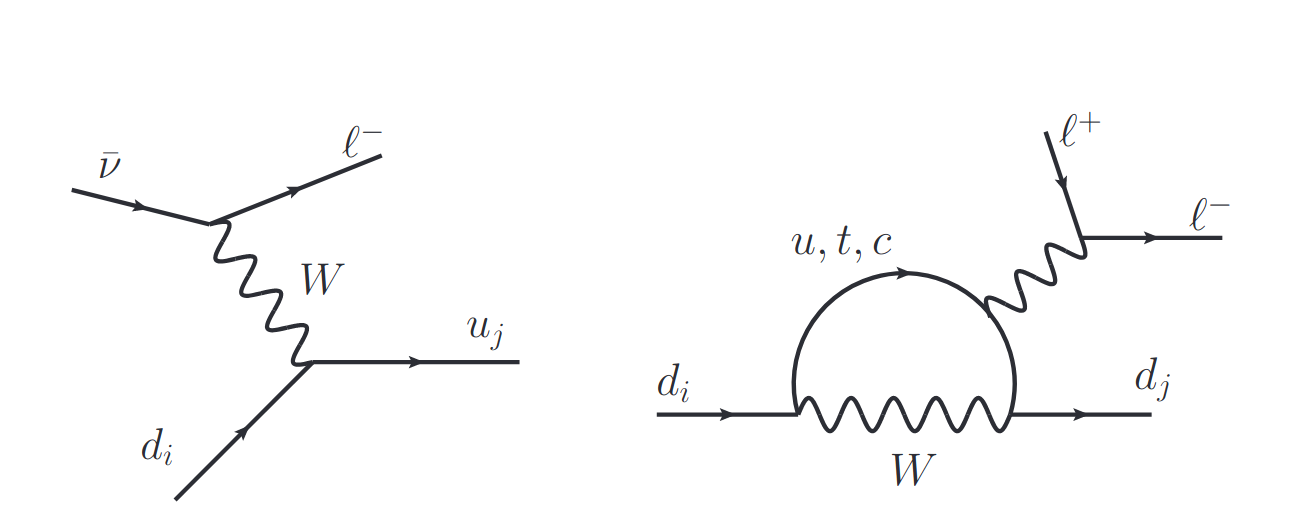
\includegraphics[width=0.75\textwidth]{Stolen.png}
	\caption{Representative tree level charged current diagram (left) and a loop induced FCNC diagram (right).}
	\label{fig:Flavour_D_1}
\end{figure}
%
%Making FCNCs virtual process.
%
Furthermore, the FCNCs come suppressed by the difference of the masses of the quarks running in the loop, $m^2_j-m^2_i$. This so called Glashow-Iliopoulos-Maiani (GIM) mechanism \cite{glashow1970weak}. Given the differences between the masses of the up and down sectors this has a significant impact. 
%
% A interesting result of this mechanism would be that that there is no flavour violation, if all the quark masses are the same. { \color{red} Relevant? }

\subsubsection{Flavour as a Probe into New Physics}

Now that we have introduced a small portion of flavor physics we can briefly touch on why collider experiments have been sold as a pathway to discovering new physics i.e. how deviation in rare decays could pin point exactly what is missing in the SM. 

Thanks to these large experiments we have many new observables in flavor physics, e.g. the branching ratios not coinciding with the SM prediction \cite{CasteloBranco2014}, observed Lepton Flavor Violation in tree and loop levels \cite{Graverini2019}.
%
As well as providing limits on processes that are prohibited in the SM but that could happen with different models, such as lepton flavor violation in Higgs decays \cite{Sirunyan_2018} in models without Lepton flavour universality. 
%
%For each of these examples there is also a plethora of different parent particles for each change of flavour, as well as many instances of final states. 
%
%The abundance of observables is clearly illustrated by opening the handy Particle Data Group (PDG) book \cite{Tanabashi2018}. 

However, one of the favored ways to search for NP is trough FCNCs this is because as mentioned there are no FCNCs at tree-level in the SM i.e. the gluon, Z and Higgs are strictly flavor conserving as we see in Fig.\,\ref{fig:QuarkCKM} at tree-level.  
%
Thus given FCNC processes are heavily suppressed in the SM trough the aforementioned GIM mechanism and loop order, and that FCNCs processes can be easily modified by NP, either through new tree level or loop level NP contributions these can serve as a good tool to search for exotic signatures. 
%
Note, these signatures could show themselves trough virtual NP particles and thus also provide evidence of high mass (Possibly TeV range) at a lower beam energy than the required energy to for one to be freely produced. 
%
This is if we assume NP can couple between generations and flavors of quarks. 

%Take the following example, if the $B_s$ meson mixing is affected by a NP process at tree-level the contribution of NP would be $\propto g^2_{sb} / M^2_{NP} $ where $g$ is the NP coupling to b and s quarks and $M_{NP}$ the mass of the new mediator.

%To shorten the discussion we will focus on the processes that are at present showing deviations from the SM expectations. 

The recipe then, seems simple, identify processes that are rare in the SM and then search for deviations from the SM predictions.
%
However, thus far all but a few processes are within $2\sigma$ experimental and theoretical bounds given by the SM. 
%
Some of the most radical being the quark level transitions, $b \rightarrow s \mu \mu$ \cite{DAmico2017}%,Geng_2017} 
 and $b \rightarrow c \tau \nu$ \cite{Hu2019} channels. %\footnote{There are other interesting ones like the $\dfrac{\epsilon^\prime}{\epsilon}$ ratio, but not quite as large \cite{Buras2015}} \cite{Fajfer_2012}
%
They are, so far, showing over $ 4 \sigma$ deviations from their expected value. 
%{\color{blue} there are very bold claims I need to better cite my work (citation needed)}.

Without going into too much depth onto the NP searches, we can examine the scale at which these processes are "integrated away". 
%
This is the energy scale at which a NP operator would allow these processes to exist only at high energies. These energies are naturally high given the terms in Eq.\,(\ref{eq:NP}). 
% Avoiding going in depth into these processes, what this might point us too, by these processes as suppressed the vector-axial processes. For them to be integrated away we get very different, but high, energy scales. There would have to exist terms a kin to, 
%If examined through V-A operators the NP scale of these 2 processes are both very different and very heavy, these would be something a kin to, 
%
\bigbreak
%
\noindent\begin{minipage}{.35\textwidth}
	\begin{figure}[H]
		\label{fig:contactNP}
		\centering
		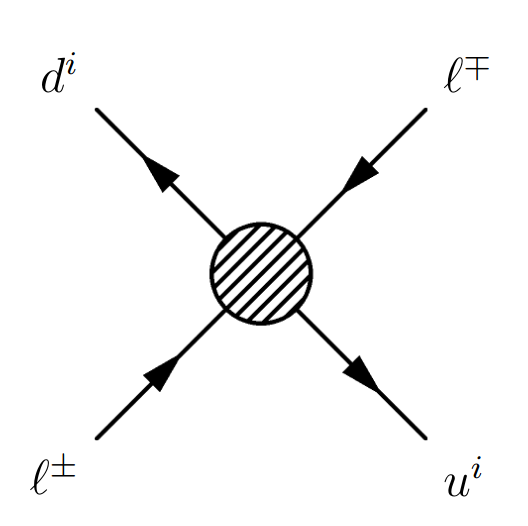
\includegraphics[width=0.6\textwidth]{My_First_Diagram.png}
		\caption{"Contact" interactions with loop interactions containing NP}
	\end{figure}
\end{minipage}
\begin{minipage}{.6\textwidth}
\begin{equation}
\label{eq:NP}
\mathcal{L}_{NP} \supset \frac{1}{\Lambda_{NP}} (\overline{Q}_i \gamma^\mu \sigma Q_j ) (\overline{L}_k \gamma_\mu \sigma L_l) ,  
\end{equation}
\end{minipage}
%
\bigbreak
%
To explain $b \rightarrow s \mu \mu$ transitions you would need a $\Lambda_{NP} \approx 3 \ \text{TeV}$ while for $b \rightarrow c \tau \nu$ you would need a $\Lambda_{NP} \approx 30\ \text{TeV}$. This is a strong indicator that some components are missing in our formulation like a new mediator for gauge interactions. The advantage of this scale is it lies almost certainly in most BSM scenarios, avoiding most experimental constraints.

As for the FCNC diagram, the $b \rightarrow s \mu \mu$ channel can be seen in Fig \ref{fig:Flavour_D_2_Muon}, 
%
\begin{figure}[H]
	\centering
	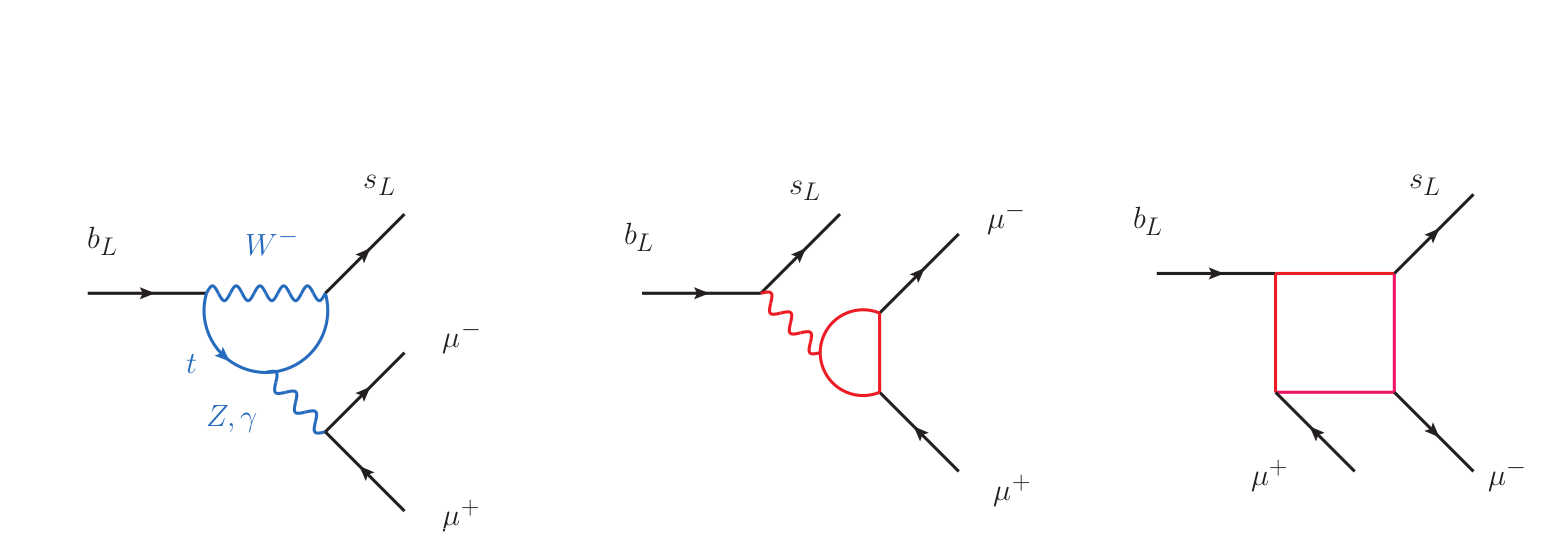
\includegraphics[width=0.95\textwidth]{Stolen_2.png}
	\caption{A representative SM diagram for $b \rightarrow s \mu \mu$ transition (left), and representative possible loop level NP
contributions (middle and right).}
	\label{fig:Flavour_D_2_Muon}
\end{figure}
%
The $b \rightarrow c \tau \nu$ flavour anomaly is similarly very clean theoretically \cite{Fajfer_2012}. However, the NP effect in these diagrams is large ($\mathcal{O}(20\%)$) compared to the SM. This means that the scale of NP needs to be lower or happen at tree-level. Consequently the NP interpretations here are often in conflict with experimental constraints, such as this decay.
%
The theoretical bias here would have been that the new charged currents are either due to a charged Higgs, $H^+$ , or a new vector boson, $W^\prime$, see Fig. \ref{fig:Flavour_D_3_Tau}. However these would have too large a effect in the $B^-$ lifetime to fully explain the anomaly according to Ref.\,\cite{Alonso_2017}.
%
\begin{figure}[H]	
	\centering
	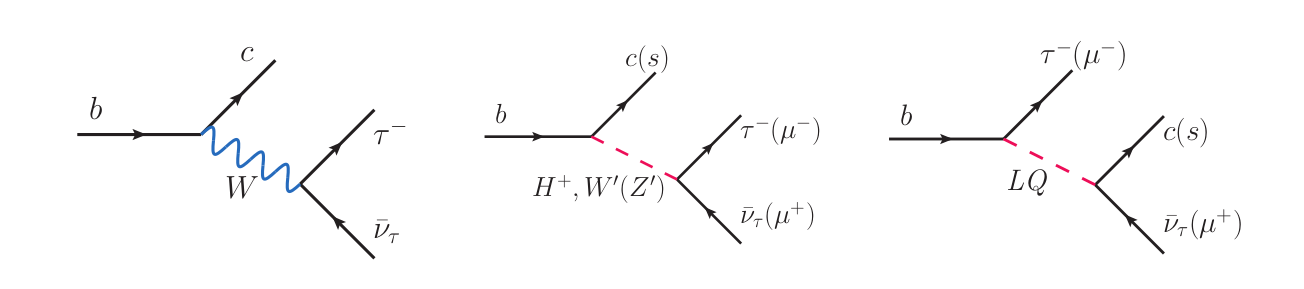
\includegraphics[width=0.95\textwidth]{Stolen_3.png}
	\caption{The SM diagrams for $b \rightarrow c \tau \nu$ transition (left), and the possible tree level NP contributions to $b \rightarrow c \tau \nu$ transition (middle and right). Where the LQ stands for a hypothetical Leptoquark particle that would interact with both leptons and quarks.}
	\label{fig:Flavour_D_3_Tau}
\end{figure}
%
Another prediction of the SM is that the rates for the  $b \rightarrow s e^+ e^-$ and  $b \rightarrow s \mu^- \mu^+$ transitions should be equal to each other.
%
The SM prediction of Lepton Flavour Universality (LFU) is deeply engrained in the structure of the theory, since it is a consequence of the fact that the electroweak gauge group is the same for all three generations. 
%
The prediction of LFU can be tested experimentally, also trough flavour physics, by theoretically clean observables such as the ratios of these flavour observables, 
%
\begin{equation}
R_{K^{\**}} = \frac{\text{Br}( B \rightarrow K^{\**} \mu^- \mu^+ )}{\text{Br} (  B \rightarrow K^{\**} e^- e^+  )} ,
\end{equation}
% 
Another strong indicator of new physics is the fact the experimental value for this ratio is $R_{K^{\**}} \approx 0.7$, violating LFU by $2.2 - 2.6 \sigma$ \cite{Wei_2009}. Revealing to yet another discrepancy between the SM and reality. 

%\subsubsection{The Future of Flavour Indirect Searches}
%
%The NP searches with rare decays, will benefit from the upcoming upgrades at Belle II and the LHC. Belle II expects to collect 50 times the Belle dataset.
%
%While for the LHC, after upgrade II aims for roughly 100 times the present data set with an upgraded detector. {\color{blue} (citation needed)}.
%
%Undoubtedly this improvement in sensibility will translate to a finer value for all measurable parameters at these experiments. We expect these anomalies then to go over the required $5 \sigma$ in future experiments (Assuming of course, they are not statistical deviations).
%
%We expect progress in leptonic decays to finally start excluding large portions of the parameter space of several models. 
%
%{ \color{red} Ask Morais: Should I add more? or remove? }


\renewcommand{\cleardoublepage}{}
\renewcommand{\clearpage}{}

\chapter{B-L-SM Model} 
\label{Chap:B-L-SM_Model}

In this chapter we introduce the minimal $\U{B-L}$ gauge extension of the SM named, the B-L-SM Model \cite{Mohapatra:1980qe} and perform a numerical analysis as to measure how it can exist in light of modern measurements. This unitary group originates from the promotion of an accidental symmetry present in the SM, the Baryon number (B) minus the Lepton number (L) to a fundamental Abelian symmetry group, incidentally, also giving the model it's name. Trough this model we are capable of explaining the generation of neutrinos masses via a simple see-saw mechanism. This see-saw is enabled by the addition of three generations of right-handed heavy Majorana neutrinos that through the new field additions are possible free of anomalies. \cite{Yanagida:1979as}. Additionally, by virtue of two new physical states, specifically a new Higgs like boson $\mathrm{H}^\prime$ and a $\mathrm{Z}^\prime$ gauge boson we can also address other phenomenology, such as deviations in EW measurements, namely the $(g-2)_\mu$ anomaly \cite{Tanabashi2018}. The additional bosons acquire mass primarily trough the spontaneous breaking of the $\U{B-L}$ symmetry that gives its name to the model. The energy scale of this breaking will also determine the mass scale for these bosons and heavy neutrinos. This (simple) mechanism for the mass generation of the referenced bosons means the model is already very heavily constrained due to long-standing direct searches at the LHC. 

{ \color{gray} Altough a deceptively simple model it can be very appealing, given that it benefits of many deep implications. Such as the fact that, through this model we can address the metastability of the EW vacuum in the SM trough the new scalar. Allowing for Higgs stabilization up to the Plank scale with a new Higgs starting from a few hundred GeVs \cite{Degrassi:2012ry}. Metastability, simply put, is the possibility of deeper minimum than the EW VEV existing in the Higgs potential. This possibility deeply affects the formation of the early universe, especially during and after inflation making it a important question for cosmologists. Note this is yet another phenomena that the SM cannot accommodate. The B-L-SM framework is also of particular interesting in the context of the study of Grand Unified Theories (GUT) as it easily embedded into higher order symmetry groups like the $\mathrm{SO(10)}$ \cite{Chanowitz:1977ye} or $\mathrm{E}_6$ \cite{Achiman:1978vg} Lie groups. Also notable is the fact that, given the presence of a new complex singlet field, $\chi$, with a Higgs doublet typically results in enhanced strength of the EW phase transition potentially converting it into a strong first-order one. This could be detectable in the form of a gravitational wave background \cite{Barger:2008jx}. Such a analysis is of utmost importance given that it could provide a way to detect NP or exclude models without the need for a larger particle collider but instead novel gravitational waves experiments, such experiments are already planned in the form of LIGO or VIGO \cite{Abbott2020}. Furthermore, the existence of heavy neutrinos is also of cosmological significance given their presence could imply the existence of a sterile state that can play the role of Dark Matter \cite{Kaneta:2016vkq}, given that, the relatively small alteration of a, $\mathbb{Z}_2$, symmetry in the neutrino sector can make these fully sterile, as seen in Ref. \cite{Okada:2018ktp}. These neutrinos can, in such case, be used to help explain the baryon asymmetry via the leptogenesis mechanism, this scenario is discussed in depth in the following Refs.~\cite{Fukugita:1986hr}.} {\color{red} delete?} 

Recall, the B-L-SM contains a family-universal symmetry in the form of, $\mathrm{U(1)_{B-L}}$, if this symmetry was introduced without changing the SM fermion content this would lead to chiral anomalies i.e a non conservative charged current on some channels involving the $\mathrm{U(1)_{B-L}}$. These are not completely undesired by themselves, as they would allow for the presence of extra sources of $\mathcal{CP}$ violation, but this inclusion at tree-level without a suppression mechanism would lead to far too much $\mathcal{CP}$ violation. 

With this in mind, we structure this chapter in the following way. First, we present the fundamental theoretical background on the model with a strong focus on the basic details of the scalar and the gauge boson mass spectra and mixing. Followed by a modern precise study of the phenomenological status of the B-L-SM model trough a layered algorithm that will be discussed preceding the results. With this algorithm we provide a numerical analysis that tests the relevant phenomenological constraints in direct and EW observables. We table off this chapter with a few representative benchmark points. 


\section{Formulating the Model}

As alluded to previously, the minimal B-L-SM is a BSM framework containing only three new ingredients, a new gauge interaction given the new symmetry group, three generations of right handed neutrinos, and a complex scalar field $\chi$. 

The particle content and related charges of the minimal $U(1)_{B-L}$ extension of the SM are shown in Tab \ref{tab:BLSM_Charges}. Note these are similar to the SM as to be expected. 
%
\begin{table}[H]
	\centering
	\begin{tabular}{|c|c|c|c|c|c|c|c|c|}
		\hline
		& $q_L$  & $u_R$ & $d_R$ & $l_L$  & $e_R$ & $\nu_R$  &  $H$  & $\chi$  \\ \hline
		$\mathrm{SU(3)_C}$& $\mathbf{3}$ & $\mathbf{3}$  & $\mathbf{3}$  & $\mathbf{1}$  & $\mathbf{1}$   & $\mathbf{1}$   & $\mathbf{1}$    & $\mathbf{1}$    \\
		$\mathrm{SU(2)_L}$& $\mathbf{2}$  & $\mathbf{1}$ & $\mathbf{1}$ & $\mathbf{2}$ & $\mathbf{1}$ & $\mathbf{1}$ & $\mathbf{2}$  & $\mathbf{1}$ \\
		$\mathrm{U(1)_Y}$ & ${1}/{6}$ & ${2}/{3}$  & -${1}/{3}$  & -${1}/{2}$ & -1 & 0 & ${1}/{2}$ & 0 \\
		$\mathrm{U(1)_{B-L}}$ & ${1}/{3}$ & ${1}/{3}$ & ${1}/{3}$  & -1  & -1 &-1  & 0 & 2  \\ \hline 
	\end{tabular}
	\caption{Quantum fields and their respective quantum numbers in the minimal B-L-SM extension. The last two lines represent the weak and $B-L$ hypercharges}
	\label{tab:BLSM_Charges}
\end{table} 


{ \color{gray} The gauge interaction is motivated by the aforementioned GUT scenarios, while a new sector of additional three $\mathrm{U(1)_{B-L}}$ charged Majorana neutrinos is essential for anomaly cancellation and generating neutrino masses.

Note, the new scalar field, $\chi$, is solely charged under $\mathrm{U(1)_{B-L}}$. This field is solely responsible for performing the breaking of the $\mathrm{B-L}$ symmetry. This is necessarily the only way to break the symmetry given that the SM-like Higgs doublet, $H$, is does not have baryon nor lepton number. The breaking of $\chi$ happens at a larger energy scale than the EW VEV. }


\subsection{Scalar sector}

Given the information presented in Tab. \ref{tab:BLSM_Charges} we can now construct all the Lagrangian terms for this theory. Much of which would be similar to the SM - we will however focus on the novel terms. We begin our study of NP in the B-L-SM by presenting the new scalar potential, which now includes two fields and reads, 
%
\begin{equation}
\label{eq:potential}
V(H,\chi) = \mu_1^2 H^\dagger H + \mu_2^2 \chi^\ast \chi + \lambda_1 (H^\dagger H)^2 + \lambda_2 \left(\chi^\ast \chi\right)^2 + \lambda_3  \chi^\ast \chi H^\dagger H \ , 
\end{equation}
%
where,  $\lambda_i$, the scalar couplings and $\mu_{1,2}^2$ the quadratic terms for $H$ and $\chi$ respectively. 
%
This potential must lead to a stable vacuum state, which means that the scalar potential must be bounded from below (BFB), i.e ensure a global minima. 
%
Such conditions can be deduced by evaluating this simple potential (Eq.\,(\ref{eq:potential})) derivatives and finding null conditions, these are commonly called tadpole equations. These conditions are seen in,
\begin{equation}
4 \lambda_1 \lambda_2  -  \lambda_3^2 > 0 \quad , \quad \lambda_1 , \lambda_2>0 
\label{eq:BFB} \ .
\end{equation}
%
The full components of the scalar fields $H$ and $\chi$ are given by,
\begin{equation}
H = \frac{1}{\sqrt{2}} 
\begin{pmatrix}
-i \( \omega_1 - i \omega_2 \) \\
v + (h + i z)
\end{pmatrix} \quad , ~\quad \chi = \frac{1}{\sqrt{2}} \( x + \(h^\prime + i z^\prime\) \) , 
\end{equation}
%
where we note that the parameters $v$ and $x$ are VEV’s associated with the $H$ and the $\chi$ field, respectively.
%
In these equations we can see that $h$ and $h^\prime$ represent the radial quantum fluctuations around the minimum of the potential.
%
These will constitute the physical degrees of freedom associated with $H$ and $H^\prime$. There are also four Goldstone directions denoted as $\omega_1$, $\omega_2$, $z$ and $z^\prime$ which are absorbed into longitudinal modes of the $W^\pm$, $Z$ and $Z^\prime$ gauge bosons once SSB takes place. 
%
After SSB the associated VEVs take the form, 
%
\begin{equation}
 \langle H \rangle = \frac{1}{\sqrt{2}} 
\begin{pmatrix}
0 \\
v 
\end{pmatrix} 
\quad , \quad
 \langle  \chi \rangle  = \frac{x}{\sqrt{2}} \ . 
\label{eq:vacuum}
\end{equation}
% 
%here, recall $v$ and $x$ are the associated VEVs to each field. 
The tadpole equations can be solved in order to each of the VEVs, returning the following Eqs.,
%
\begin{equation}
	v^2 = \tfrac{-\lambda_2 \mu_1^2 + \tfrac{\lambda_3}{2}\mu_2^2}{\lambda_1 \lambda_2 - \tfrac{1}{4}\lambda_3^2} > 0
	\qquad
	\text{and}
	\qquad
	x^2 = \tfrac{-\lambda_1 \mu_2^2 + \tfrac{\lambda_3}{2}\mu_1^2}{\lambda_1 \lambda_2 - \tfrac{1}{4}\lambda_3^2} > 0 , 
	\label{eq:extremum}
\end{equation}
%
which, when simplified with the BFB conditions yield a simpler set of equations,
%
\begin{equation}
\lambda_2 \mu_1^2 < \tfrac{\lambda_3}{2} \mu_2^2 
\qquad
\text{and}
\qquad
\lambda_1 \mu_2^2 < \tfrac{\lambda_3}{2} \mu_1^2 \ . 
\label{eq:sols}
\end{equation}
%
Note that although $\lambda_1$ and $\lambda_2$ must be positive to ensure the correct conical shape of the potential, no such conditions exist for the sign of $\lambda_3$ , $\mu_1$, and $\mu_2$. However observing Eq\,(\ref{eq:sols}) we can infer that only some combinations of signs are impossible, 
%
\begin{table}[H]
	\begin{center}
		\begin{tabular}{ccccc}
			& $\mu_2^2 > 0$ & $\mu_2^2 > 0$ & $\mu_2^2 < 0$ & $\mu_2^2 < 0$  	\\
			& $\mu_1^2 > 0$ & $\mu_1^2 < 0$ & $\mu_1^2 > 0$ & $\mu_1^2 < 0$  	\\        
			\hline  
			$\lambda_3 < 0 $     			    							& 	\xmark		& \checkmark	&	\checkmark & \checkmark	\\
			$\lambda_3 > 0$     			    							& \xmark		& \xmark	&	\xmark &  \checkmark \\
			\hline
		\end{tabular} 
		\caption{Possible signs of the potential parameters in Eq\,(\ref{eq:potential}). 
The \checkmark\,symbol indicates the existence of solutions for tadpole conditions Eq.\,\eqref{eq:sols}, while the \xmark\,indicates unstable configurations.}
		\label{tab:signs}  
	\end{center}
\end{table} 
%
For our numerical analysis we decided to leave the sign of $\lambda_3$ positive, choosing a configuration where both $\mu$ parameters are negative. 
%
This does not directly translate to any real physical consequence.  

With these conditions now established we proceed to investigate the physical states of the B-L-SM scalar sector. 
%
At the vacuum, we evaluate the Hessian matrix as,
%
\begin{equation}
\mathbf{M}^2 =
\begin{pmatrix}
4 \lambda_2 x^2 & \lambda_3 v x \\ 
\lambda_3 v x   & 4 \lambda_1 v^2 
\end{pmatrix}\,.
\label{eq:hess}
\end{equation}
% 
Moving this matrix to its physical mass eigenbase, we obtain the following eigenvalues,
%
\begin{equation}
m_{h_{1,2}}^2 = \lambda_1 v^2 + \lambda_2 x^2 \mp \sqrt{(\lambda_1 v^2 - \lambda_2 x^2)^2 + (\lambda_3 x v)^2}.
\label{eq:eigvals}
\end{equation}
The physical basis vectors $h_1$ and $h_2$ can then be related to the original fields of gauge eigenbasis $h$ and $h^\prime$ trough a simple rotation matrix:
%
\begin{equation}
	\begin{pmatrix}
	h_1 \\
	h_2 
	\end{pmatrix}
	=
	\mathbf{O}
	\begin{pmatrix}
	h \\
	h^\prime 
	\end{pmatrix},
	\label{eq:trans}
\end{equation}
%
where $\mathbf{O}$ can be parameterized by a single mixing angle $\alpha_h$,
%
\begin{equation}
	\mathbf{O} = 
	\begin{pmatrix}
	\cos \alpha_h & -\sin \alpha_h \\
	\sin \alpha_h & \cos \alpha_h 
	\end{pmatrix}\,.
	\label{eq:rotmat}
\end{equation}
%
%The precise mixing angle is represented simply by, 
%\begin{equation}
%\tan 2 \alpha_h   = \frac{ \left| \lambda_3 \right|  v x }{  \lambda_2 x^2 -\lambda_1 v^2 } 
%\end{equation} 
%
It is particularly interesting to analyze the scenario where the scalar fields approximately decouple, that is, in the limit, $v/x\ll 1$. In these circumstances, the scalar masses and the mixing angle become rather simple,
\begin{equation}
\sin \alpha_h \approx \dfrac{1}{2}\dfrac{\lambda_3}{\lambda_2} \dfrac{v}{x} \quad , \quad 
m_{h_1}^2 \approx 2 \lambda_1 v^2 \quad , \quad m_{h_2}^2 \approx 2 \lambda_2 x^2
\label{eq:simplify} .
\end{equation}
%
We will see in the context of our numerical results that for a phenomenologically consistent mass scale these equations serve as a valid approximation for most of the points. 

\subsection{Gauge Sector}

Moving onto the gauge boson and Higgs kinetic terms in the B-L-SM, consider the following portion of the Lagrangian,
\begin{equation}
\mathcal{L}_{\mathrm{U(1)'s}} =  \left| D_\mu H \right|^2 + \left| D_\mu \chi \right|^2 -\dfrac{1}{4} F_{\mu \nu} F^{\mu \nu} -\dfrac{1}{4} F^\prime_{\mu \nu} F^{\prime \mu \nu} -\dfrac{1}{2} \kappa F_{\mu \nu} F^{\prime \mu \nu} , 
\label{eq:Lu1}
\end{equation}
where $F^{\mu \nu}$ and $F^{\prime \mu \nu}$ are the standard field strength tensors, respectively for the $\U{Y}$ and  $\U{B-L}$ Abelian groups, 
\begin{equation}
	F_{\mu \nu} = \partial_\mu A_\nu - \partial_\nu A_\mu 
	\qquad
	\text{and}
	\qquad
	 F^\prime_{\mu \nu} = \partial_\mu A^\prime_\nu - \partial_\nu A^\prime_\mu\,,
	 \label{eq:Fmn}
\end{equation}
written in terms of the gauge fields $A_\mu$ and $A_\mu^\prime$, respectively. Given that this is a model with two Unitary groups, without a parity symmetry ($\mathbb{Z}_2$) to prevent it, we must consider the possible mixing in between them. In this work we parameterized this mixing trough a parameter $\kappa$.

With this goal in mind consider the Abelian portion of the covariant derivative in Eq.\,(\ref{eq:Lu1}) is given by,
\begin{equation}
	D_\mu \supset i g_1 Y A_\mu + i g_1^\prime Y_{\rm B-L} A_\mu^\prime\,,
\end{equation} 
% 
with $g_1$ and $g_1^\prime$ the $\U{Y}$ and $\U{B-L}$ the gauge couplings with the $Y$ and $B-L$ charges are specified in Tab.\ref{tab:BLSM_Charges}. It is convenient to rewrite the gauge kinetic terms in the canonical form, i.e.
%
\begin{equation}
	F_{\mu \nu} F^{\mu \nu} + F^\prime_{\mu \nu} F^{\prime \mu \nu} + 2 \kappa F_{\mu \nu} F^{\prime \mu \nu} \to B_{\mu \nu} B^{\mu \nu} + B^\prime_{\mu \nu} B^{\prime \mu \nu}\,.
	\label{eq:AtoB}
\end{equation}
%
A generic orthogonal transformation in the field space does not eliminate the kinetic mixing term. So, in order to satisfy Eq.~\eqref{eq:AtoB} an extra non-orthogonal transformation should be imposed such that Eq.~\eqref{eq:AtoB} is realized. Taking $\kappa = \sin \alpha$, a suitable redefinition of fields $\{A_\mu,A_\mu^\prime\}$ into $\{B_\mu, B_\mu^\prime\}$ that eliminates $\kappa$-term according to Eq.~\eqref{eq:Lu1} can be cast as
\begin{equation}
	\begin{pmatrix}
	A_\mu \\
	A^\prime_\mu 
	\end{pmatrix}
	=
	\begin{pmatrix}
	1 & -\tan \alpha \\
	0 & \sec \alpha 
	\end{pmatrix}
	\begin{pmatrix}
	B_\mu \\
	B^\prime_\mu 
	\end{pmatrix}\,.
	\label{eq:trans-kappa}
\end{equation}
Note there is a limit without kinetic mixing where $\alpha = 0$. Note that this transformation is generic and valid for any basis in the field space. The transformation (\ref{eq:trans-kappa}) results in a modification of the covariant derivative that acquires two additional terms encoding the details of the kinetic mixing, i.e.

\begin{equation}
D_\mu \supset \partial_\mu + i \(g_Y \; Y + g_BY \; Y_{B-L}\) B_\mu + i \(g_{B-L} \; Y_{B-L} + g_{YB} \; Y\) B_\mu^\prime\,,
\label{eq:newCov}
\end{equation}	
where the gauge couplings take the form
\begin{equation}
	g_Y = g_1 \quad , \quad 
	g_{B-L} = g_1^\prime \sec \alpha   \quad , \quad 
	g_{YB} = -g_1 \tan \alpha  \quad , \quad 
	g_{BY} = 0 \,,  
	\label{eq:new-g-simp}
\end{equation}
%
which is the standard convention in the literature.
%
Note that this definition is merely to simplify the equations and has no physical impact. 
%
We will later see that this kinetic mixing is a desired feature and why stabilizing it with a $\mathbb{Z}_2$ symmetry would be detrimental in terms of depth.
%
The resulting mixing between the neutral gauge fields including $Z^\prime$ can be represented as follows
%
\begin{equation}
\begin{aligned}
\begin{pmatrix}
\gamma_\mu \\
Z_\mu \\
Z^\prime_\mu
\end{pmatrix}
=
\begin{pmatrix}
\cos \theta_W & \sin \theta_W & 0\\
-\sin \theta_W \cos \theta_W^\prime & \cos \theta_W \cos \theta_W^\prime & \sin \theta_W^\prime \\
\sin \theta_W \sin \theta_W^\prime & -\cos \theta_W^\prime \sin \theta_W^\prime & \cos \theta_W^\prime
\end{pmatrix}
\begin{pmatrix}
B_\mu \\
A^3_\mu \\
B^\prime_\mu
\end{pmatrix} , 
\end{aligned}
\label{eq:g-Z-Zp}
\end{equation}
%
where $\theta_W$ is the weak mixing angle and $\theta^\prime_W$ is defined as
\begin{equation}
\sin(2 \theta^\prime_W) = \frac{2 g_{YB} \sqrt{g^2 + g_{Y}^2}}{\sqrt{(g_{YB}^2 + 16 (\frac{x}{v})^2 g_{B-L}^2 - g^2 - g_{Y}^2)^2 + 4 g_{YB}^2 (g^2 + g_{Y}^2)} }\,,
\label{eq:theta-p-full}
\end{equation}
%
in terms of $g$ and $g_{Y}$ being the $\mathrm{SU(2)_{L}}$ and $\mathrm{U_{Y}}$ gauge couplings, respectively. In the physically relevant limit, $v/x \ll 1$, the above expression greatly simplifies leading to
%
\begin{equation}
	\sin \theta_W^\prime \approx \dfrac{1}{16
	} \dfrac{g_{YB}}{g_{B-L}}\( \dfrac{v}{x} \)^2 \sqrt{g^2 + g_{Y}^2} \,,
	\label{eq:theta-p}
\end{equation}
%
up to $(v/x)^3$ corrections. In the limit of no kinetic mixing, i.e. $g_{YB} \to 0$, there is no mixture of $Z^\prime$ and SM gauge bosons. 

Note, that the kinetic mixing parameter $\theta_W^\prime$ has rather stringent constraints from $Z$ pole experiments both at the Large Electron-Positron Collider (LEP) and the Stanford Linear Collider (SLC), restricting its value to be smaller than $10^{-3}$ approximately \cite{Bandyopadhyay_2018}, which we set as an upper bound in our numerical analysis. 

Finally we can, trough the expansion of the kinetic terms $\left| D_\mu H \right|^2 + \left| D_\mu \chi \right|^2$ around the vacuum, extract the following mass matrix for the vector bosons
\begin{equation}
	m_V^2 =
	\dfrac{v^2}{4}
	\begin{pmatrix}
	g^2 \;\;&\;\; 0 \;\;&\;\; 0 \;\;&\;\; 0 \;\;&\;\; 0 \\
	0 \;\;&\;\; g^2 \;\;&\;\; 0 \;\;&\;\; 0 \;\;&\;\; 0 \\
	0 \;\;&\;\; 0 \;\;&\;\; g^2 \;\;&\;\; -g g_{Y} \;\;&\;\; -g g_{YB} \\
	0 \;\;&\;\; 0 \;\;&\;\; -g g_{Y} \;\;&\;\; g_{Y}^2 \;\;&\;\; g_{Y} g_{YB} \\
	0 \;\;&\;\; 0 \;\;&\;\; -g g_{YB} \;\;&\;\; g_{Y} g_{YB} \;\;&\;\; g_{YB}^2 + 16 \(\dfrac{x}{v}\)^2 g_{B-L}^2
	\end{pmatrix} , 
\end{equation}
%
whose, first set of eigenvalues read,
\begin{equation}
	m_A = 0 \quad \text{,} \quad m_W = \tfrac{1}{2} v g \ , 
\end{equation}
corresponding to the expected physical photon and $W^\pm$ bosons. While the following set,
\begin{equation}
m_{Z,Z^\prime}=\sqrt{g^2 + g^2_{Y}} \cdot \frac{v}{2}  \sqrt{\frac{1}{2} \left( \frac{g_{YB}^2 + 16 (\frac{x}{v})^2 g^2_{\rm BL} }{g^2 + g^2_{\rm Y}} +1  \right) \mp \frac{g_{YB}}{\sin(2 \theta_W^\prime) \sqrt{g^2 + g^2_{\rm Y}}}}\,,
\label{eq:ZZp-mass}
\end{equation}
correspond to two neutral massive vector bosons, with one of them, not necessarily the lightest, representing the SM-like $Z$ boson. It follows from LEP and SLC constraints on $\theta_W^\prime$, that Eq.~\eqref{eq:theta-p} also implies that either $g_{YB}$ or the ratio ${v}/{x}$ are small. In this limit, Eq.~\eqref{eq:ZZp-mass} simplifies to
\begin{equation}
	m_Z \approx \tfrac{1}{2} v \sqrt{g^2 + g_{Y}^2} \qquad \text{and} \qquad m_{Z^\prime} \approx 2 g_{B-L} x\,,
	\label{eq:mZ}
\end{equation}
%
where the $m_{Z^\prime}$ depends only on the SM-singlet VEV ,$x$ and on the $\mathrm{U(1)_{B-L}}$ gauge coupling and will be attributed to a heavy $Z^\prime$ state, while the light $Z$-boson mass corresponds to its SM value.

\subsection{The Yukawa Sector}

One of the key features of the B-L-SM model is the presence of non-zero neutrino masses. 
%
In its minimal version, such masses are generated via a type-I seesaw mechanism, thus producing a very light neutrino for each of the three known flavors, and a corresponding heavy neutrino one for each, which we theorize are yet to be observed.
%
In the type-I seesaw mechanism the mixing of neutrinos fields is written with similar shape to, 
\begin{equation}
\left( \begin{array}{c|c}
0 & A \\
\midrule
A & B 
\end{array} \right) . 
\end{equation}
This system would have a set eigenvalues written as, 
\begin{equation}
\lambda_\pm = \frac{ B \pm \sqrt{B^2 + 4 A} }{ 2 } \ . 
\end{equation}
Investigating the nature of these eigenvalues allows us to understand the see-saw process.
%
The mean of these values being always equal to $|B|$, if one value goes up, another goes down, like a see-saw. $B$ is set to be proportional to Majorana mass terms, orders of magnitude higher than the cross-terms $A$. Given this, the smaller eigenvalue, is, 
\begin{equation}
\lambda_- \approx \frac{A^2}{B} . 
\end{equation}
This mechanism serves to explain why the neutrino masses are so small if there exists a much heavier partner in the see-saw. 

The total Yukawa Lagrangian of the model reads,
\begin{equation}
\begin{aligned}
\mathcal{L}_f = 
-Y_u^{ij} \bar{q}_{\rm L i} u_{\rm R j} \widetilde{H} 
-Y_d^{ij} \bar{q}_{\rm L i} d_{\rm R j} H
-Y_e^{ij} \bar{\ell}_{\rm L i} e_{\rm R j} H
- Y_\nu^{ij} \bar{\ell}_{\rm L i} \nu_{\rm R j} \widetilde{H}
	-\dfrac{1}{2} Y_\chi^{ij} \overline{\nu}_{\rm R i}^c \nu_{\rm R j} \chi + {\rm H.c.} \ . 
\end{aligned}
\label{eq:Yuk}
\end{equation}
%
Notice the explicit lack of Majorana neutrino mass terms of the form $M \overline{\nu_{R}^c} \nu_{R}$. 
These explicitly violate the $\mathrm{U(1)_{B-L}}$ symmetry and are therefore not present. 
In Eq.~\eqref{eq:Yuk}, $Y_u$, $Y_d$ and $Y_e$ are the $3 \times 3$ Yukawa matrices that reproduce the quark and charged lepton sector exactly the same way as in the SM, while $Y_\nu$ and $Y_\chi$ are the new Yukawa matrices responsible for the generation of right handed neutrino masses and mixing with left handed fields.
%
In particular, one can write,
\begin{equation}
	\mathbf{m}_{\nu_l}^{\text{Type-I}} = \dfrac{1}{\sqrt{2}}\dfrac{v^2}{x} \mathbf{Y}_\nu^t \mathbf{Y}^{-1}_\chi \mathbf{Y}_\nu\,,
\end{equation}
%
for light $\nu_l$ neutrino masses, whereas the heavy $\nu_h$ ones are given by
\begin{equation}
	\mathbf{m}_{\nu_h}^{\text{Type-I}} \approx \dfrac{1}{\sqrt{2}} \mathbf{Y}_\chi x\,,
\end{equation} 
where we have assumed a flavor diagonal basis.

Note that the smallness of light neutrino masses imply that either the $x$ VEV is very large or (if we fix it to be at the $\mathcal{O}\left({\mathrm{TeV}}\right)$ scale and $\mathbf{Y}_\chi \sim \mathcal{O}\(1\right)$) the corresponding Yukawa coupling should be tiny, $\mathbf{Y}_\nu < 10^{-6}$. 
%
It is clear that the low scale character of the type-I seesaw mechanism in the minimal B-L-SM is \textit{faked} by small Yukawa couplings to the Higgs boson. A more elegant description was proposed in Ref.~\cite{Khalil:2010iu} where small SM neutrino masses naturally result from an inverse seesaw mechanism.
%
In this work, however, we will not study the neutrino sector and thus, for an improved efficiency of our numerical analysis of $Z^\prime$ observables, it will be sufficient to fix the Yukawa couplings to $\mathbf{Y}_\chi = 10^{-1}$ and $\mathbf{Y}_\nu = 10^{-7}$ values such that the three lightest neutrinos lie in the sub-eV domain.


\section{Numerical Results}

Given the nature of this model, much work has already been performed on it. We would then like to point-out the recent work done by our colleges in Ref. \cite{Deppisch:2019ldi}. Where a comprehensive study for the $Z^\prime$ at the LHC is performed, in particular, from $0.2 \ \mathrm{GeV}$ to $200 \ \mathrm{GeV}$. As for slightly heavier $Z^\prime$ masses beyond $m_{Z^\prime} \gtrsim 100~\mathrm{GeV}$, the combined effect of the EW precision observables and the ATLAS searches for Drell-Yan $Z^\prime$ production decaying into di-leptons, i.e.~$pp \to Z^\prime \to ee,\mu \mu$ \cite{Aaboud:2017buh}, is also finely investigated. We then endeavored to achieve a complementary study where we investigated the case of very heavy $Z^\prime$ bosons. 

Our goal is to see if the case of an heavy $Z^\prime$, whose kinect mixing is highly constrained by LHC experimental results, can provide additional phenomenological implications besides the addition of a new unobserved vector boson trough this portal. This was chiefly done by the investigation of the $\left(g-2\right)_\mu$ anomaly. We examine the relations that this anomaly has with the parameter space, such as gauge couplings, as well as the extra scalar mass. 

%\subsubsection{The $\left( g-2 \right)_\mu$ anomaly refers}

The $\left( g-2 \right)_\mu$ anomaly refers to the discrepancy between the measured anomalous magnetic moment of the muon, $a_\mu^{\mathrm{\text{exp}}} \equiv \tfrac{1}{2} \left( g-2 \right)^{\mathrm{\text{exp}}}_\mu$, and its theoretical prediction, $a_\mu^{\mathrm{SM}} \equiv \tfrac{1}{2} \left(g-2\right)^{\mathrm{SM}}_\mu$, which reads \cite{Tanabashi:2018oca}
%
\begin{equation}
	\label{g-2}
	\Delta a_\mu = a_\mu^{\ro{exp}} - a_\mu^{\ro{SM}} = 268(63)(43) \times 10^{-11}
\end{equation}
%
with numbers in brackets denoting experimental and theoretical errors, respectively. This represents a deviations of $3.5$ standard deviations from the combined $1 \sigma$ error and is calling for new physics effects beyond the SM theory. 

There is a strong possibility that through radiative corrections a new gauge bosons could explain this deviation \cite{Czarnecki:2001pv}. In fact a version of this study has already been performed in the supersymmetrical version of the B-L-SM \cite{Yang:2018guw}. 

In the B-L-SM, NP contributions to $a_\mu$, denoted as $\Delta a_\mu^{\textrm{NP}}$ in what follows, can emerge from the diagrams containing $Z^\prime$ or $h_2$ propagators. New physics contributions $\Delta a_\mu^{\ro{NP}}$ to the muon anomalous magnetic moment are given at one-loop order by the Feynman diagrams depicted in Fig.~\ref{fig:g-2}. 
\begin{figure}[H]
	\centering
	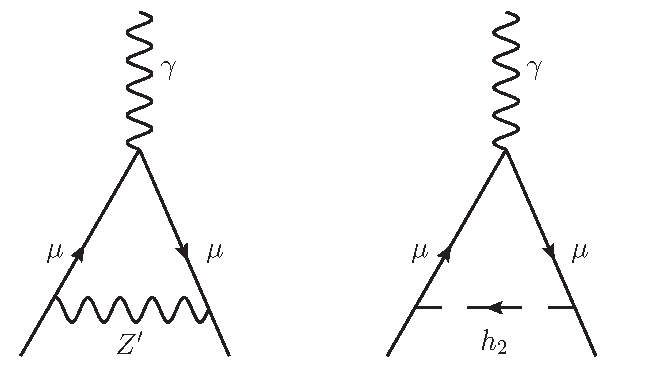
\includegraphics[scale=0.5]{/BLSM/g-2.pdf}
	\caption{NP one-loop diagrams contributing to $\Delta a_\mu^{\ro{NP}}$ in the B-L-SM.}
	\label{fig:g-2}
\end{figure}	
%%%%%%%%%%%%%%%%%%%%%%%%%


\subsection{The Scanning Apparatus}

The numerical data presented in this section was generated via a large chain of nested scripts. These were created as a first generation of a scanning framework for generic phenomenological models. This machinery later expanded and improved for the 3HDM portion of the thesis, so much of this introduction will be glossed over in the 3HDM section, as much remained the same. 

The underlying code is a mixture of Linux bash and Python 3 scripts, and utilizes \texttt{SPheno 4.0.3} \cite{Porod:2011nf},  \texttt{SARAH 4.13.0} \cite{Staub:2013tta}, \texttt{HiggsBounds 4.3.1} \cite{Bechtle:2013wla}, \texttt{HiggsSignals 1.4.0} \cite{Bechtle:2013xfa} and \texttt{MadGraph5\_aMC@NLO 2.6.2} \cite{Alwall:2014hca} programs/packages. 

These scripts generate a Monte-Carlo type scan through a desired parameter space. Unless introduced, all non-relevant physical constants and parameters are defined in a way as to keep the observed gauge, lepton and quark structure. { \color{gray} Skipping a bit ahead, as an example, for the B-L-SM scan our routine randomly samples parameter space points according to the ranges in Tab.~\ref{tab:scan} while keeping things like Higgs doublet VEV and Weinberg angle to reproduce the correct $W$ and $Z$ structure. } 

Given the randomness in our scan, we can reach nonphysical, or nonsensical regions, that contain objects like tachyonic scalar masses un-renormalizable quantities, divergent radiative corrections etc. 
%
These points must be rejected before even considering experimental constraints. This is done by automatically by a prepackaged setting in \texttt{SPheno}. 
%
We could consider this our first layered check. 

While a second layer of tests include the phenomenological studies we shall perform. 
%
This is the region where we confront the surviving scenarios with experimental data. 
%
Such as precision measurements from the oblique $S,T,U$ parameters and constraining the Higgs Sector to reproduce the observed signal seen in the LHC in 2012. 
%
The latter is made automatically trough the package \texttt{HiggsBounds 4.3.1} that shall be used to apply a $95\%$ C.L. exclusion limit cut on a new scalar particle, $h_2$, while \texttt{HiggsSignals 1.4.0} is used to calculate and later check, through a $\chi^2$ distribution, the probability for consistency with the observed Higgs boson signal data. 
% 
To calculate these variables \texttt{HiggsBounds 4.3.1} and \texttt{HiggsSignals 1.4.0} are provided all scalar masses, total decay widths, Higgs decay branching ratios as well as the SM-normalized effective Higgs couplings to fermions and bosons squared (that are needed for analysis of the Higgs boson production cross sections). For details about this calculation, see Ref.~\cite{Bechtle:2013wla}.

{ \color{gray} After setting a random set of parameters \texttt{SPheno} will generate all relevant data for our analysis if possible. \texttt{SPheno} is a particle spectrum generator code written in Fortran 90. Its emphasis on easy generalisability and speed made it a natural part of our numerical analysis. It takes information about our models Lagrangian, such as fields, charges and fundamental symmetries, and creates a executable file capable of quickly generating a spectrum file with all details regarding mass, decay and flavour observables information in the standardized SUSY Les-Houches accord format. All generated spectrums are processed and stored. 
%
This Lagrangian information is fed to \texttt{SPheno} also in standardized format automatically generated by a Mathematica packaged designed for such purposes called \texttt{SARAH}. }

On a third and final layer of phenomenological tests we have studied the viability of the surviving scenarios from the perspective of direct collider searches for a new $Z^\prime$ gauge boson. 
%
We have used, the popular \texttt{MadGraph5\_aMC@NLO}, to compute the $Z^\prime$ Drell-Yan production cross section and subsequent decay into the first and second-generation leptons, i.e.~$ \sigma\left(pp \to Z^\prime\right) \times B\left(Z^\prime \to \ell \ell\right)$ with $\ell = e,\; \mu$, and then compare our results to the most recent ATLAS exclusion bounds from the LHC runs at the center-of-mass energy $\sqrt{s} = 13~\ro{TeV}$ \cite{Aaboud:2017buh}. 
%
The \texttt{SPheno} SLHA output files were used as parameter cards for \texttt{MadGraph5\_aMC@NLO}, where the information required to calculate $ \sigma\left(pp \to Z^\prime\right) \times B\left(Z^\prime \to \ell \ell\right)$, such as the $Z^\prime$ boson mass, its total width and decay branching ratios into lepton pairs, is provided. 
%
The lepton anomalous magnetic moments $\left( g-2 \right)_\ell /2 \equiv a_\ell$ are calculated in \texttt{SPheno} at one-loop order. Note, despite these diagrams being one-loop order all masses are calculated at 2-loop order in \texttt{SPheno}.  


\subsection{Numerical discussion}

For the B-L-SM scan our routine randomly samples parameter space points according to the ranges in Tab.~\ref{tab:scan}.
%
\begin{table}[H]
	\begin{center}
%\begin{ruledtabular}
		\begin{tabular}{ccccc}
			\toprule                     
			$\lambda_{1}$ & $\lambda_{2,3}$ & $g_{\mathrm{B-L}}$ & $g_{\mathrm{YB}}$ & $x~{\mathrm{[TeV]}}$  
			\\       
						\midrule 
			$\left[10^{-2},\; 10^{0.5}
			\right]$ 			    							& $\left[10^{-8},\; 10
			\right]$ 			    							& $\left[10^{-8},\; 10
			\right]$		& $\left[10^{-8},\; 10
			\right]$	&	$\left[0.5,\; 20.5
			\right]$ 	\\
			\bottomrule
		\end{tabular}  
		\caption{Parameter scan ranges used in our analysis. Note that the value of $\lambda_1$ is mostly constrained by the tree-level Higgs boson mass given in Eq.~\eqref{eq:simplify}. 
		}
		\label{tab:scan}
%\end{ruledtabular}
	\end{center}
\end{table}

\subsubsection{Electroweak Precision Observables}
\label{Sec:B-L-SM-EW}
Typically, the most stringent constraints of the scalar sector emerge from the oblique $S,T,U$ parameters, which are also calculated by \texttt{SPheno}. 
%
This conecept was first introduced by Peskin and T. Takeuchi in Ref\,\cite{Peskin1992}.
%
Current precision measurements provide the allowed regions,
%
\begin{equation}
	S = 0.02 \pm 0.10\,, \qquad T = 0.07 \pm 0.12\,, \qquad U = 0.00 \pm 0.09 \ ,
	\label{eq:oblique}
\end{equation}
%
where $S$-$T$ are $92\%$ correlated, while $S$-$U$ and $T$-$U$ are $-66\%$ and $-86\%$ anti-correlated, respectively.
%
We compare our results with the EW fit in Eq.~\eqref{eq:oblique} and require consistency with the best fit point within a $95\%$ C.L.~ellipsoid (see Ref.~\cite{Costa:2014qga} for further details about this method). %
%
The contributions coming from NP can be calculated trough,
%
\begin{equation}
\Delta \chi \equiv \sum_{ij}  \left(  \Delta \mathcal{O}_{i}^{NP} - \mathcal{O}_{i}^{(0)} \right) [ ( \sigma^2 )^{-1} ]_{ij}  \left(  \mathcal{O}_{j}^{NP} - \mathcal{O}_{j}^{(0)}  \right) < 7.815 \ , 
\end{equation}
%
where $\Delta \mathcal{O}_i^{NP} \equiv \mathcal{O}_i - \mathcal{O}^{SM} \rightarrow (\Delta S , \Delta T , \Delta U )$ and $\mathcal{O}_i^{(0)}$ is the deviation generated by the Higgs doublet in the SM if his mass is 125.09. Finally the covariance matrix expressed in terms of correlation matrix and started deviations can be seen in, 
\begin{equation}
[ \sigma^2 ]^{-1} \equiv \begin{pmatrix}
867.49 & -904.30 & -360.66\\
-904.30 & 1154.65 & 584.55 \\
-360.66 & 584.55 &  455.19
\end{pmatrix} . 
\end{equation}
These values are taken from \cite{Baak_2012}. 

We show in Fig.~\ref{fig:STU} our results in the $ST$ (left) and $TU$ (right) planes where black points are consistent with EW precision observables at $95\%$ C.L.~whereas grey ones lie outside the corresponding ellipsoid of the best fit point and, thus, the first points to be excluded in our analysis. 
%%%%%%%%%%%%%%%%%%%%%%%%%
\begin{figure}[H]
	\centering
	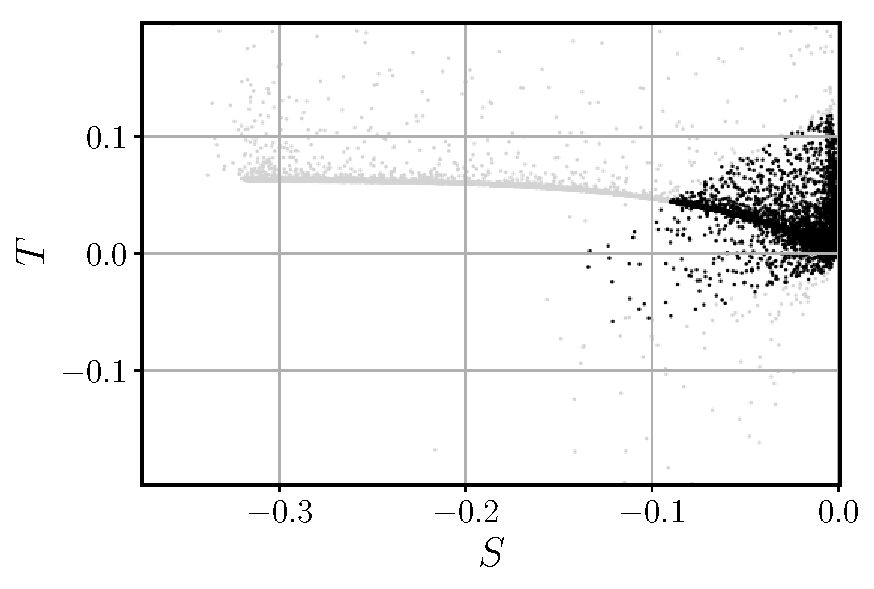
\includegraphics[scale=0.45]{/BLSM/ST.pdf}
	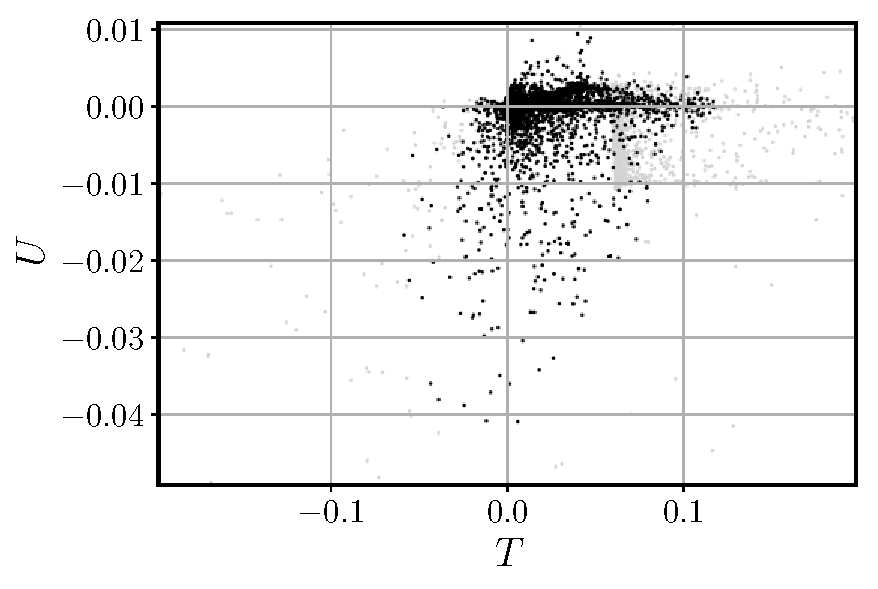
\includegraphics[scale=0.45]{/BLSM/TU.pdf}
	\caption{B-L-SM scatter plots for EW precision observables showing the $ST$ (left) and $TU$ (right) planes. Accepted points lying within a $95\%$ C.L.~ellipsoid of the best fit point are represented in black whereas grey points are excluded.}
	\label{fig:STU}
\end{figure}	
%%%%%%%%%%%%%%%%%%%%%%%%%

%The B-L-SM predicts a new visible scalar, which we denote as $h_2$, in addition to a SM-like $125~\ro{GeV}$ Higgs boson, $h_1$. 

\subsubsection{Higgs Constraints}

We then confront the surviving scenarios (black points in Fig.~\ref{fig:STU}), with collider bounds on Higgs searches at the LHC, LEP and the Tevatron trough \texttt{HiggsBounds 4.3.1} and \texttt{HiggsSignals 1.4.0}. 
%
Additionally we also ensured that a SM Higgs candidate is assured, $m_{h_1} = 125.10 \pm 0.14~\textrm{GeV}$. 

%The basic value calculated by \texttt{HiggsSignals} is the signal strength modifier $\mu_{x}$ which parameterizes the signal rate of a particular final state $x$ normalized to the SM expectation trougha a peak-centered $\chi^2$ statistical method.

%The combined implementation of \texttt{HiggsBounds/HiggsSignals}, looks at the properties of the discovered Higgs and searches for additional Higgs states, which are then either excluded or allowed in the particle spectra of our model. 

\subsubsection{$Z^\prime$ Constraints}

Trough the previously mentioned process we can now look at the viability of the surviving points from the perspective of direct collider searches for a new $Z^\prime$ gauge boson. Enabling the discussion of the phenomenological properties of the B-L-SM model. We can see the impact of all layered cuts in the following figures reflecting Higgs and Gauge physics cuts. We show in Fig.~\ref{fig:Plots1} the scenarios generated in our parameter space scan that have passed all theoretical and experimental.
%
%%%%%%%%%%%%%%%%%%%%%%%%%
\begin{figure}[H]
	\centering
	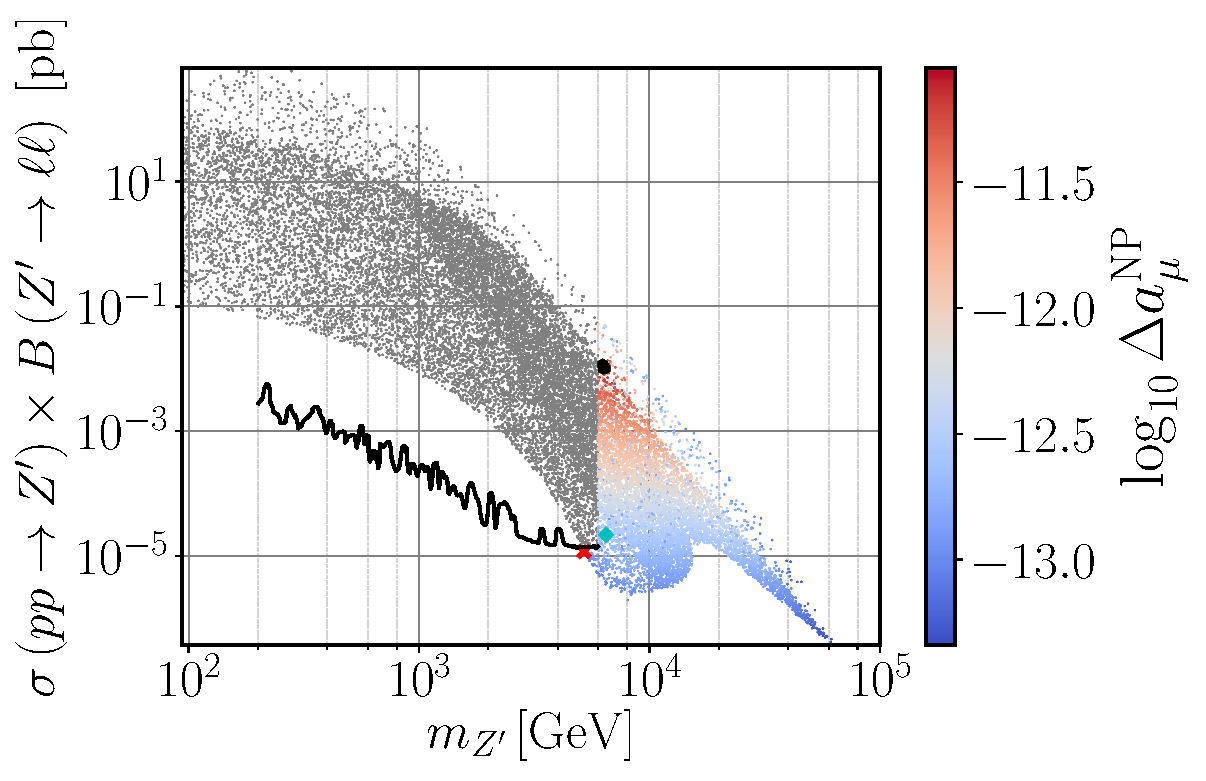
\includegraphics[scale=0.37]{/BLSM/mZp_Xsec_Amu.pdf}
	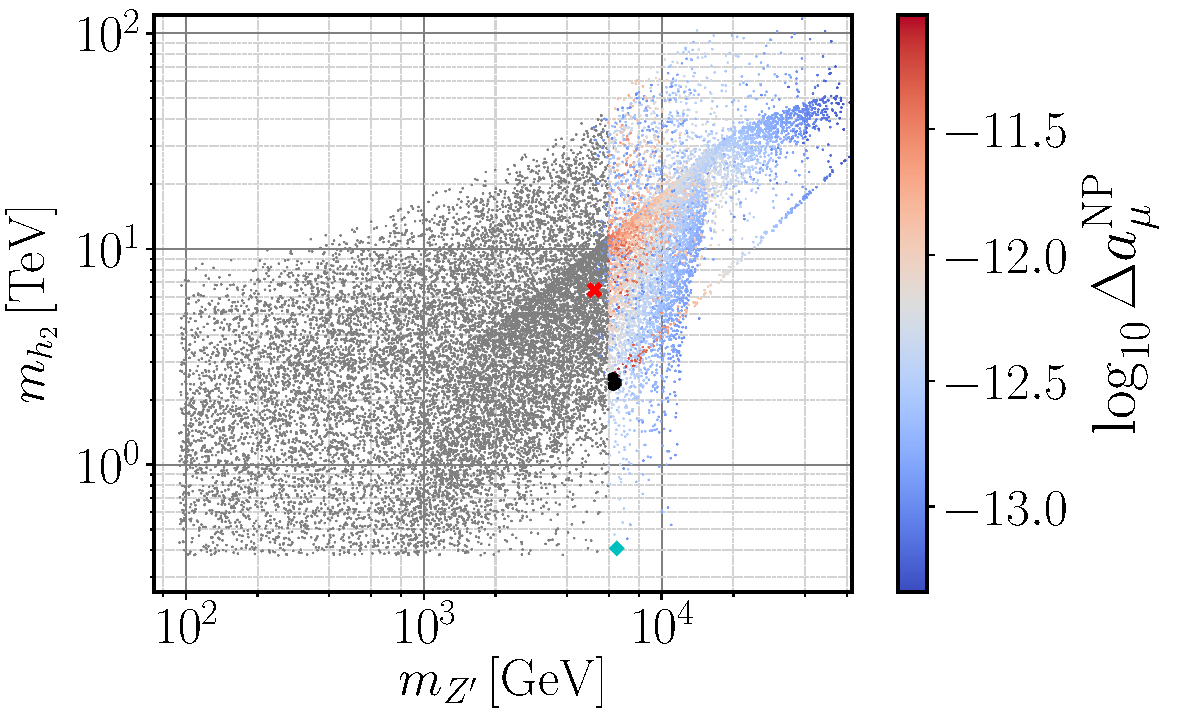
\includegraphics[scale=0.37]{/BLSM/mZp_Mhp_Amu.pdf}
	\caption{Scatter plots showing the $Z^\prime$ Drell-Yan production cross section times the decay branching ratio into a pair of electrons and muons (left panel) and the new scalar mass $m_{h_2}$ (right panel) as functions of $m_{Z^\prime}$ and the NP contributions to the muon $\Delta a_\mu$ anomaly. Coloured points have survived all theoretical and experimental constraints while grey points are excluded by direct $Z^\prime$ searches at the LHC. The region between the two dashed lines represents the current ATLAS expected limit on the production cross section times branching ratio into a pair of leptons at $95\%$ C.L.~and is taken from the plot in Fig.~4 of Ref.~\cite{Aaboud:2017buh}. The four highlighted points in both panels denote the benchmark scenarios described in detail in Tab.~\ref{tab:bench}.}
	\label{fig:Plots1}
\end{figure}	
%%%%%%%%%%%%%%%%%%%%%%%%%

Here, on the left panel, we show the $Z^\prime$ production cross section times its branching ratio to the first - and second-generation leptons, $\sigma B \equiv \sigma \left( pp \to Z^\prime \right) \times B \left( Z^\prime \to \ell \ell \right) $ with $\ell = e,\mu$, as a function of the new vector boson mass and the new physics contribution to the muon anomalous magnetic moment $\Delta a^{\textrm{NP}}_\mu$ (color scale). 
%
On the right panel, we show the new scalar mass, $m_{h_2}$, as a function of the $Z^\prime$ Mass. 
%
All points above the red dashed line are excluded at $95\%$ C.L.~by the upper expected limit on $Z^\prime$ direct searches at the LHC by the ATLAS experiment and are represented in gray shades. 
%
Darker shades denote \textit{would-be-scenarios} with larger values of $\Delta a^{\textrm{NP}}_\mu$ while the smaller contributions to the muon $\left(g-2\right)_\mu / 2$ anomaly are represented with the lighter shades. 
%
The region between the two dashed lines corresponds to the $Z^\prime$ ATLAS limit with a $2\sigma$ uncertainty represented by the yellow band in Fig.~4 of \cite{Aaboud:2017buh}.
%
Provided that the observed limit by the ATLAS detector lies within this region we have taken a conservative approach and accepted all points whose $\sigma B$ value lies below the red dashed line (upper limit) in Fig.~\ref{fig:Plots1}.
%
The blue dashed line, which corresponds to the stricter $2 \sigma$ lower bound, is only shown for completeness of information. The red cross in our figures signals the lightest $Z^\prime$ found in our scan which we regard as a possible early-discovery (or early-exclusion) benchmark point in the forthcoming LHC runs. Such a benchmark point is shown in the first line of Tab.~\ref{tab:bench}.
%
On the right panel, we notice that the new scalar bosons can become as light as $380 - 400~\textrm{GeV}$, but with $Z^\prime$ masses in the range of $5 - 9~\textrm{TeV}$. We highlight with a magenta diamond the benchmark point with the lightest $Z^\prime$ boson within this range. 
%
This point is shown in the second line of Tab.~\ref{tab:bench}.
%
\begin{table}[H]
	\begin{center}
	%\resizebox{\columnwidth}{!}{%
%\begin{ruledtabular}
		\begin{tabular}{cccccccc}
			% \toprule                     
			$m_{Z^\prime}$ & $m_{h_2}$ &  $x$ & $ \log_{10} \Delta a_\mu^{\ro{NP}}$ & $\sigma B$ & $\theta_W^\prime$ & $\alpha_h$ & $g_{\ro{B-L}} \simeq g^{\ell \ell Z^\prime}$ \vspace{1mm}
			\\
			\hline \vspace{-2mm} \\ 
			%%%%%%%%%%
			$3.13$ 			    							& $3.72$ 			    				& $15.7$		& $-12.1$	&	$2.22\times 10^{-4}$ &	$\approx 0$ &	$5.67 \times 10^{-5}$ &	$0.0976$\vspace{1mm} 	\\
			%%%%%%%%%%
			$5.37$ 			    							& $0.396$ 			    				& $9.10$		& $-11.7$	&	$4.23 \times 10^{-5}$ &	$2.55 \times 10^{-7}$ &	$9.44 \times 10^{-7}$ &	$0.302$\vspace{1mm}  	\\
			%%%%%%%%%%
			$7.35$ 			    							& $1.49$ 			    				& $0.321$		& $-8.75$	&	$0.0115$ &	$1.83 \times 10^{-7}$ &	$1.20 \times 10^{-6}$ &	$3.15$\vspace{1mm}  	\\
			%%%%%%%%%%
			$5.91$ 			    							& $1.32$ 			    				& $0.335$		& $-8.78$	&	$0.0285$ &	$1.30 \times 10^{-4}$ &	$1.04 \times 10^{-5} $ &	$2.94$\vspace{1mm}  	\\
%			\bottomrule
		\end{tabular}
%		\end{ruledtabular}
		%}
		\caption{A selection of four benchmark points represented in Figs.~\ref{fig:Plots1}, \ref{fig:Plots4} to \ref{fig:Plots2}. The $m_{Z^\prime}$, $m_{h_2}$ and $x$ parameters are given in TeV. The first line represents a point with light $h_2$ while the second line shows the lightest allowed $Z^\prime$ boson found in our scan. The last two lines show two points that reproduce the observed value of the muon $(g-2)$ within $1\sigma$ uncertainty.}
		\label{tab:bench}
	\end{center}
\end{table}
% 
\subsubsection{Implications of direct $Z^\prime$ searches at the LHC for the $\left(g-2\right)_\mu$ anomaly}

Looking again to Fig.~\ref{fig:Plots1} (left panel), we see that there is a thin dark-red stripe where $\Delta a^{\ro{NP}}_\mu$ explains the observed anomaly shown in Eq.~(\ref{g-2}) for a range of $m_{Z^\prime}$ boson masses approximately between $5~\ro{TeV}$ and $20~\ro{TeV}$. This region is particularly interesting as it can be partially probed by the forthcoming LHC runs or at future colliders. If a $Z^\prime$ boson discovery remains elusive for such a mass range, it can exclude a possibility of explaining the muon $\left(g-2\right)_\mu$ anomaly in the context of the B-L-SM. It is also worth noticing that such preferred $\Delta a^{\ro{NP}}_\mu$ values represent a small island in the right plot of Fig.~\ref{fig:Plots1} where the new scalar boson mass is restricted to the range of $1~\ro{TeV} < m_{h_2} < 4~\ro{TeV}$.

Since the couplings of a new scalar $h_2$ to the SM fermions are suppressed by a factor of $\sin \alpha_h$, which we find to be always smaller than $0.08$ as can be seen in the bottom panel of Fig.~\ref{fig:Plots4}, the right diagram in Fig.~\ref{fig:g-2}, which scales as $\Delta a_\mu^{h_2} \propto {m_\mu^2}/{m_{h_2}^2}\left(y_\mu \sin \alpha_h\right)^2$ with $\sin^2 \alpha_h < 0.0064$ and $y_\mu = Y_e^{22}$, providing sub-leading contributions to $\Delta a_{\mu}$. Furthermore, as we show in the top-left panel of Fig.~\ref{fig:Plots4} the new scalar boson mass, which we have found to satisfy $m_{h_2} \gtrsim 380~\ro{GeV}$, is not light enough to compensate the smallness of the scalar mixing angle. 
%%%%%%%%%%%%%%%%%%%%%%%%%
\begin{figure}[H]
	\centering
	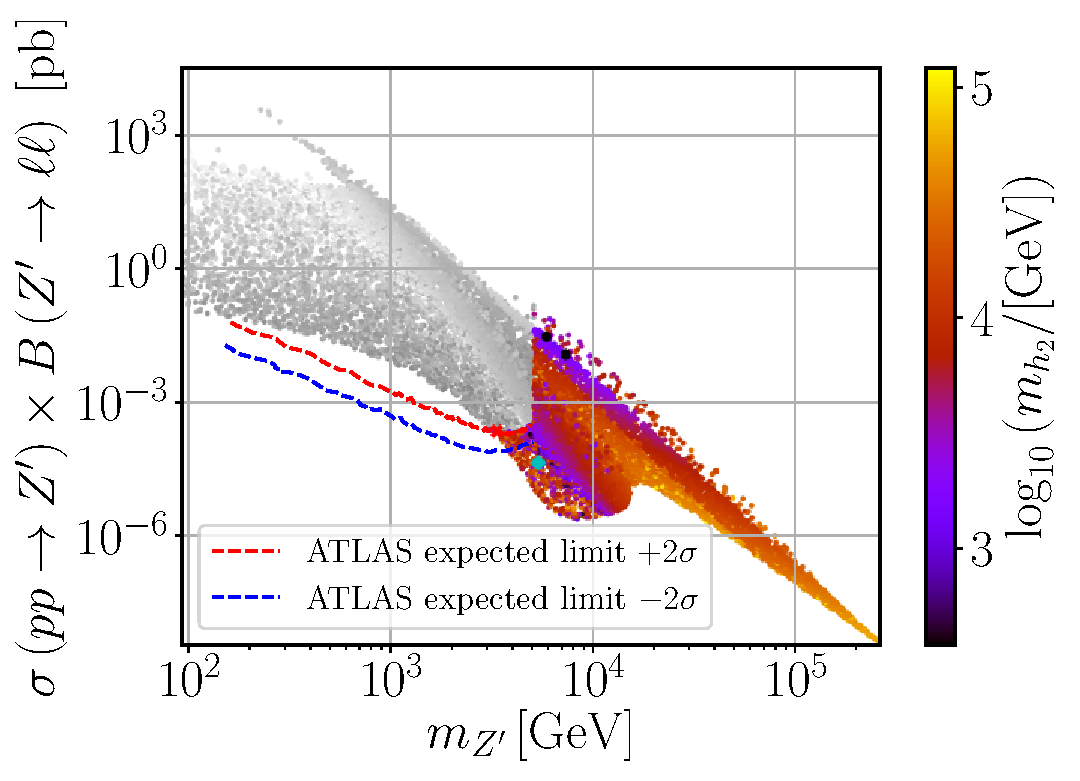
\includegraphics[scale=0.37]{/BLSM/mZp_Xsec_mh2.pdf}
	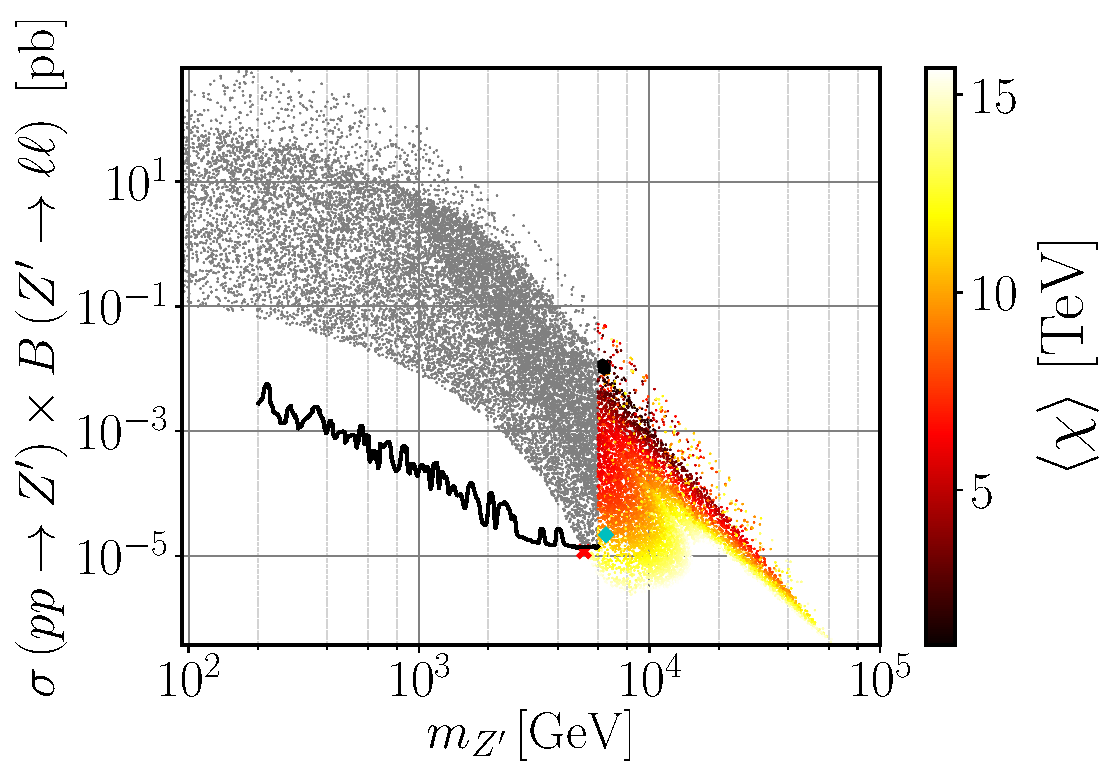
\includegraphics[scale=0.37]{/BLSM/mZp_Xsec_VEV.pdf}
	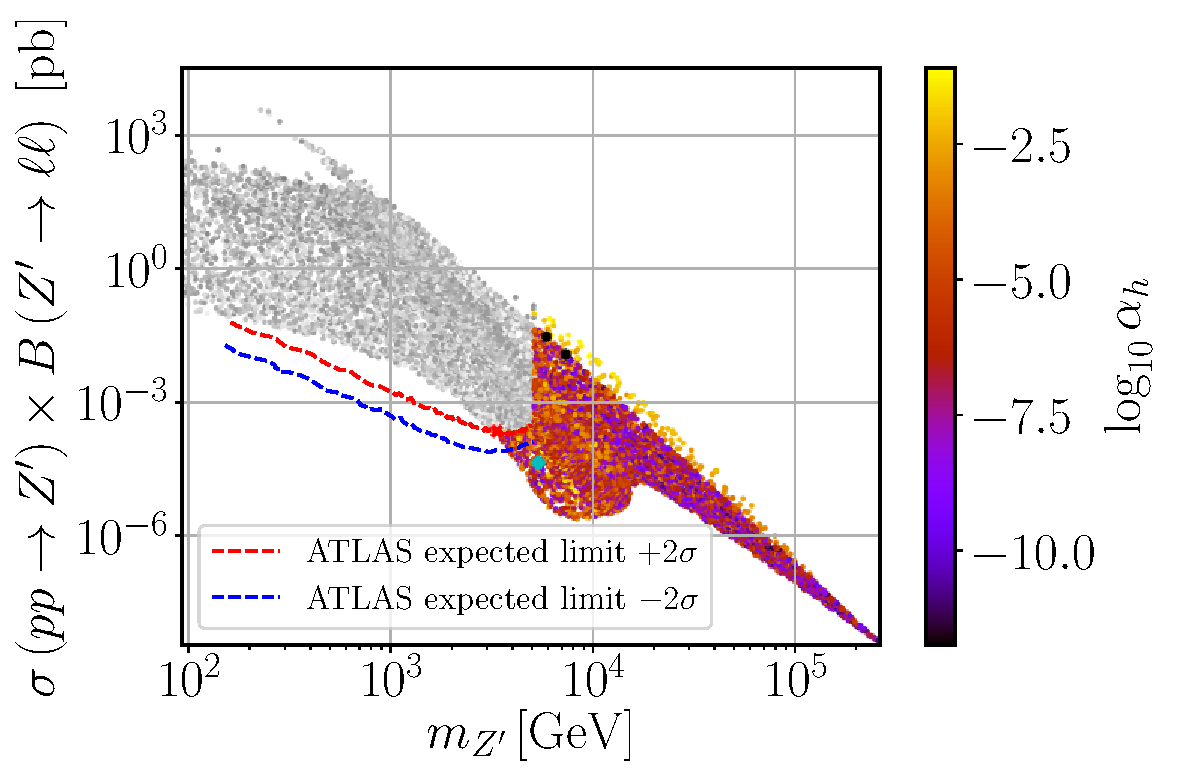
\includegraphics[scale=0.37]{/BLSM/mZp_Xsec_alpha.pdf}	
	\caption{Scatter plots showing the $Z^\prime$ Drell-Yan production cross section times the decay branching ratio into a pair of electrons and muons in terms of the $m_{Z^\prime}$ boson mass. The colour gradation represents the new scalar mass (top-left), the ratio between the EW- and $\U{B-L}$-breaking VEVs (top-right) and the scalar mixing angle (bottom). The grey points are excluded by direct $Z^\prime$ searches at the LHC. The four benchmark points in Tab.~\ref{tab:bench} are represented by the black dots (last two rows), cyan diamond (first row) and red cross (second row).}
	\label{fig:Plots4}
\end{figure}	
%%%%%%%%%%%%%%%%%%%%%%%%%
Conversely,  the new $Z^\prime$ boson can have sizeable couplings to fermions via gauge interactions proportional to $g_{\rm B-L}$. Therefore, the left diagram in Fig.~\ref{fig:g-2} provides the leading contribution to the $\left(g-2\right)_\mu$ in the model under consideration. The $\Delta a_\mu^{Z^\prime}$ contribution coming from the $Z^\prime$ is given by \cite{Freitas:2014pua}
\begin{equation}
\Delta a_\mu^{Z^\prime} = \tfrac{1}{12 \pi^2} \tfrac{m_{\mu}^2}{m_{Z^\prime}^2} \(3 g_{\rm L}^{\mu \mu Z^\prime} g_{\rm R}^{\mu \mu Z^\prime} - {g_{\rm L}^{\mu \mu Z^\prime}}^2 - {g_{\rm R}^{\mu \mu Z^\prime}}^2 \) ,
\label{eq:ZpContribution}
\end{equation}
where the left- and right-chiral projections of the charged lepton couplings to the $Z^\prime$ boson, $g_{\rm L}^{\ell \ell Z^\prime}$ and $g_{\rm R}^{\ell \ell Z^\prime}$, respectively, can be approximated as follows,
\begin{equation}
\begin{aligned}
    g_{\rm L}^{\ell \ell Z^\prime} &\simeq g_{\rm B-L} + \tfrac{1}{32} \(\tfrac{v}{x}\)^2 \tfrac{g_{\rm YB}}{g_{\rm B-L}} \[g_{\rm Y}^2 - g^2 + 2 g_{\rm Y}g_{\rm YB}\]\,,
    \\
    g_{\rm R}^{\ell \ell Z^\prime} &\simeq g_{\rm B-L} + \tfrac{1}{16} \(\tfrac{v}{x}\)^2 \tfrac{g_{\rm YB}}{g_{\rm B-L}} \[g_{\rm Y}^2 + g_{\rm Y}g_{\rm YB}\]\,,
\end{aligned}\label{eq:gllZ}
\end{equation}
to second order in $v/x$-expansion. If $v/x \ll 1$, corresponding to the darker shades of the color scale in the top-right panel of Fig.~\ref{fig:Plots4}, we can further approximate
%
\begin{equation}
    g_{\rm L}^{\ell \ell Z^\prime} \simeq g_{\rm R}^{\ell \ell Z^\prime} \simeq g_{\ro{B-L}}\,,
    \label{eq:gLgR-simp}
\end{equation}
%
such that the muon anomalous magnetic moment gets significantly simplified to
\begin{equation}
\Delta a_\mu^{Z^\prime} \simeq \dfrac{g_{\ro{B-L}}^2}{12 \pi^2} \dfrac{m_{\mu}^2}{m_{Z^\prime}^2}\,.
\label{eq:amu-simple}
\end{equation}
%
Similarly, for the yellow band in the bottom of Fig.~\ref{fig:Plots3}, which corresponds to the region where $\Delta a_{\mu}^{\rm NP}$ is maximized (see top-left panel of Fig.~\ref{fig:Plots1}), a large value of the $\U{B-L}$ gauge coupling also allows one to simplify Eq.~\eqref{eq:ZpContribution} reducing it to the form of Eq.~\eqref{eq:amu-simple}. This is in fact what we have observed and, for the yellow band region, we see in the bottom panel of Fig.~\ref{fig:Plots3} that $g_{\ro{B-L}} \simeq 3$. A sizeable value of $g_{\ro{B-L}}$ is indeed what is contributing to the enhancement of $\Delta a_{\mu}^{\rm NP}$, in particular, for the red region in both panels of Fig.~\ref{fig:Plots1}. We show in the third and fourth lines of Tab.~\ref{tab:bench} the two benchmark points that better reproduce the muon anomalous magnetic moment represented by two black dots in
Figs.~\ref{fig:Plots1}, \ref{fig:Plots4} to \ref{fig:Plots2}.
%%%%%%%%%%%%%%%%%%%%%%%%%
\begin{figure}[H]
	\centering
	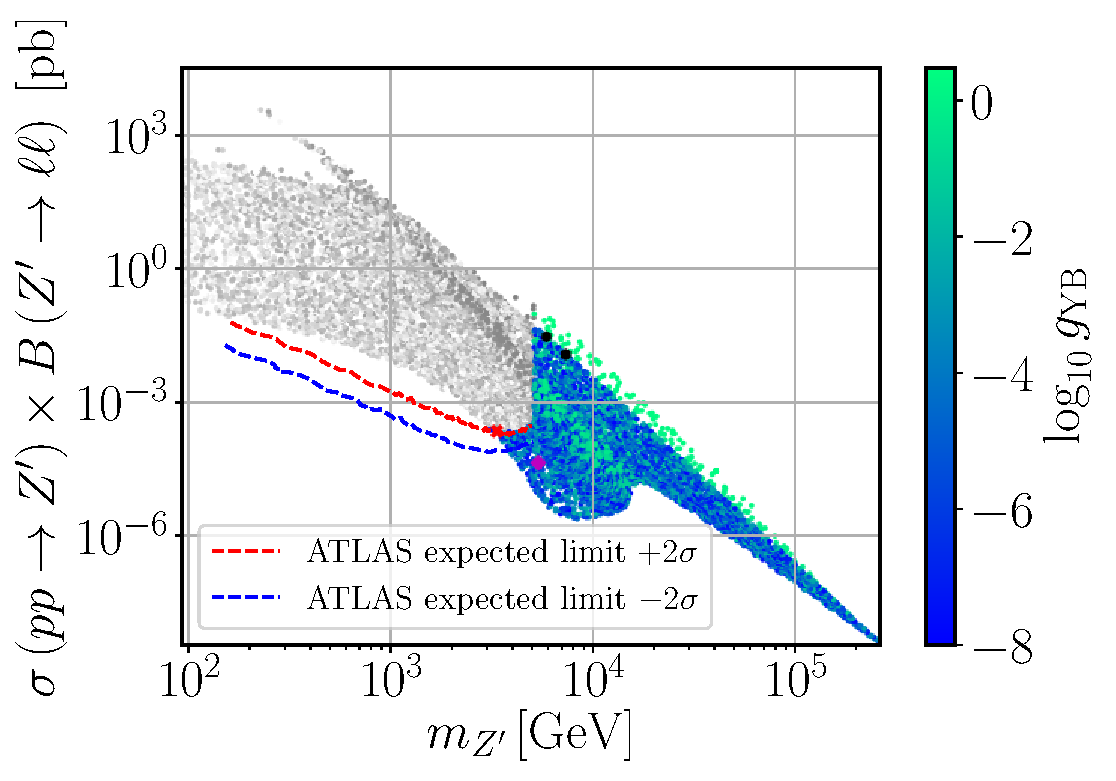
\includegraphics[scale=0.37]{/BLSM/mZp_Xsec_gYB.pdf}
	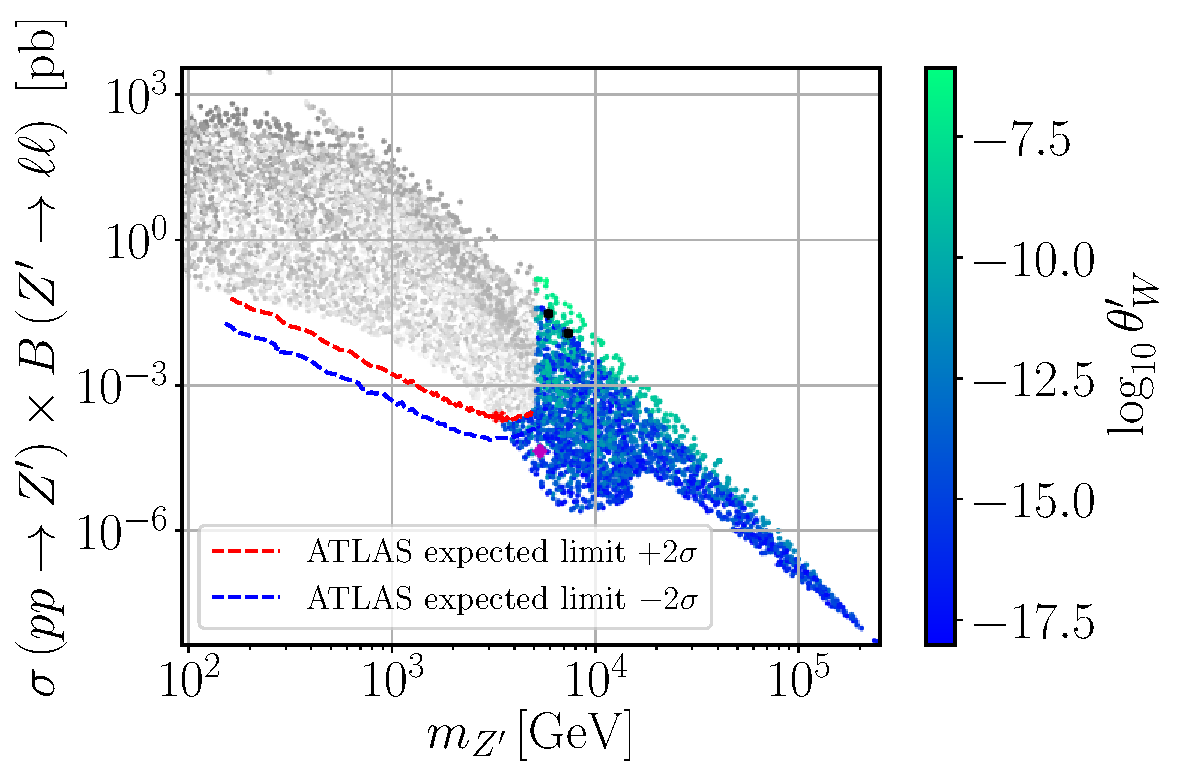
\includegraphics[scale=0.37]{/BLSM/mZp_Xsec_twp.pdf}
	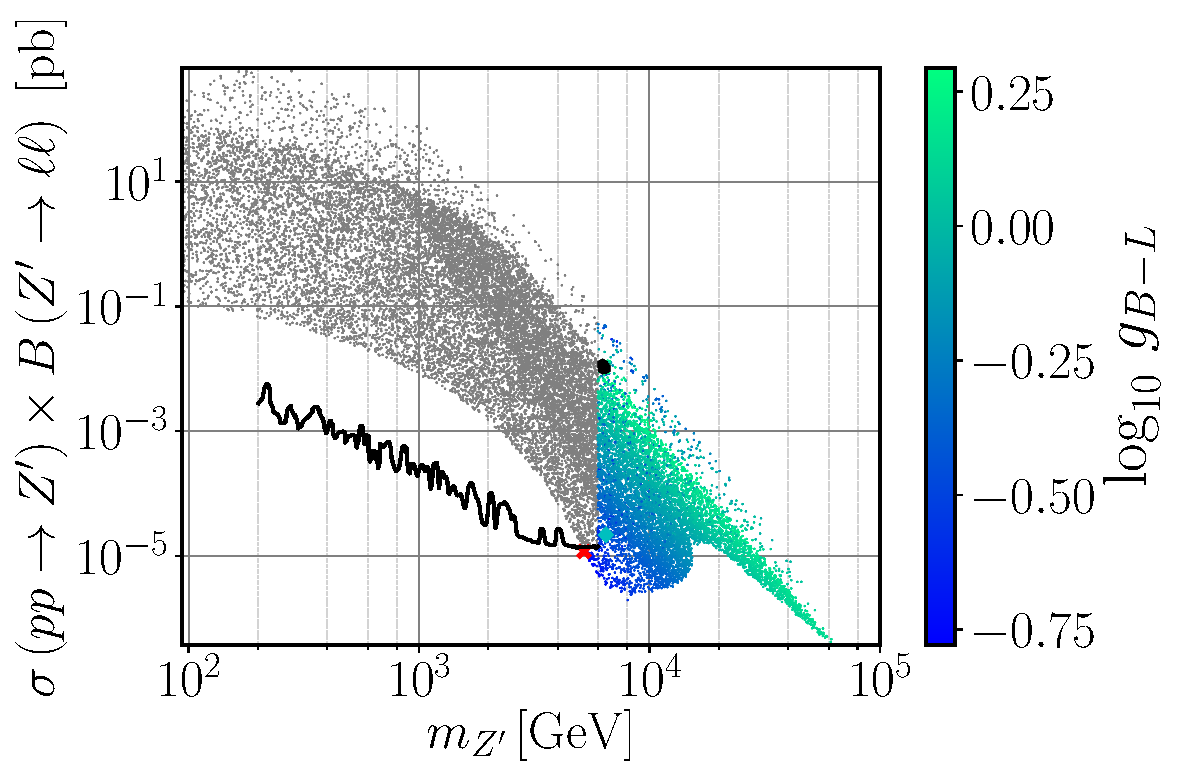
\includegraphics[scale=0.37]{/BLSM/mZp_Xsec_gBL.pdf}	
	\caption{The same as in Fig.~\ref{fig:Plots4} but with the colour scale representing the gauge-mixing parameters $g_{\ro{YB}}$ (top-left), $\theta_{W}^{\prime}$ (top-right), and the $\U{B-L}$ gauge coupling (bottom).}
	\label{fig:Plots3}
\end{figure}	
%%%%%%%%%%%%%%%%%%%%%%%%%

In fact, a close inspection of Fig.~\ref{fig:Plots1} (left panel) and Fig.~\ref{fig:Plots4} (top-right panel) reveals an almost one-to-one correspondence between the colour shades. 
This suggests that $\Delta a_{\mu}^{Z^\prime}$ must somehow be related to the VEV ratio $v/x$. 
To understand this behaviour, let us also look to Fig.~\ref{fig:Plots3} (top-left panel) where we see that the kinetic-mixing gauge coupling $g_{\ro{YB}}$ is typically very small apart from two green bands where it can become of order $\mathcal{O}(1)$.
Interestingly, whenever $g_{\ro{YB}}$ becomes sizeable, $v/x \ll 1$ is realised, which means that Eq.~\eqref{eq:mZ} is indeed a good approximation as was argued above. It is then possible to eliminate $g_{\ro{B-L}}$ from Eq.~\eqref{eq:amu-simple} and rewrite it as
\begin{equation}
    \Delta a_\mu^{Z^\prime} \simeq \dfrac{y_\mu^2}{96 \pi^2} \(\dfrac{v}{x}\)^2 \,,
    \label{eq:amu-vev}
\end{equation}
which explains the observed correlation between both Fig.~\ref{fig:Plots1} (left panel) and Fig.~\ref{fig:Plots4} (top-right panel) and, for instance, the thin red stripe of points is compatible with a full description of the muon $\left(g-2\right)_{\mu}/2$ anomaly. Note that this simple and illuminating relation becomes valid as a consequence of the heavy $Z^\prime$ mass regime, in combination with the smallness of the $\theta_{W}^{\prime}$ mixing angle required by LEP constraints. Indeed, while we have not imposed any strong restriction on the input parameters of our scan (see Tab.~\ref{tab:scan}), Eq.~\eqref{eq:theta-p} necessarily implies that both $g_{\ro{YB}}$ and $v/x$ cannot be simultaneously sizeable in agreement with what is seen in Fig.~\ref{fig:Plots3} (top-left panel) and Fig.~\ref{fig:Plots4} (top-right panel). The values of $\theta_W^\prime$ obtained in our scan are shown in the top-right panel of Fig.~\ref{fig:Plots3}.

{ \color{gray}
For completeness, we show in Fig.~\ref{fig:Plots2} the physical couplings of $Z^\prime$ to muons (top panels) and to $W^\pm$ bosons (bottom panel).
%%%%%%%%%%%%%%%%%%%%%%%%%
\begin{figure}[!htb]
	\centering
	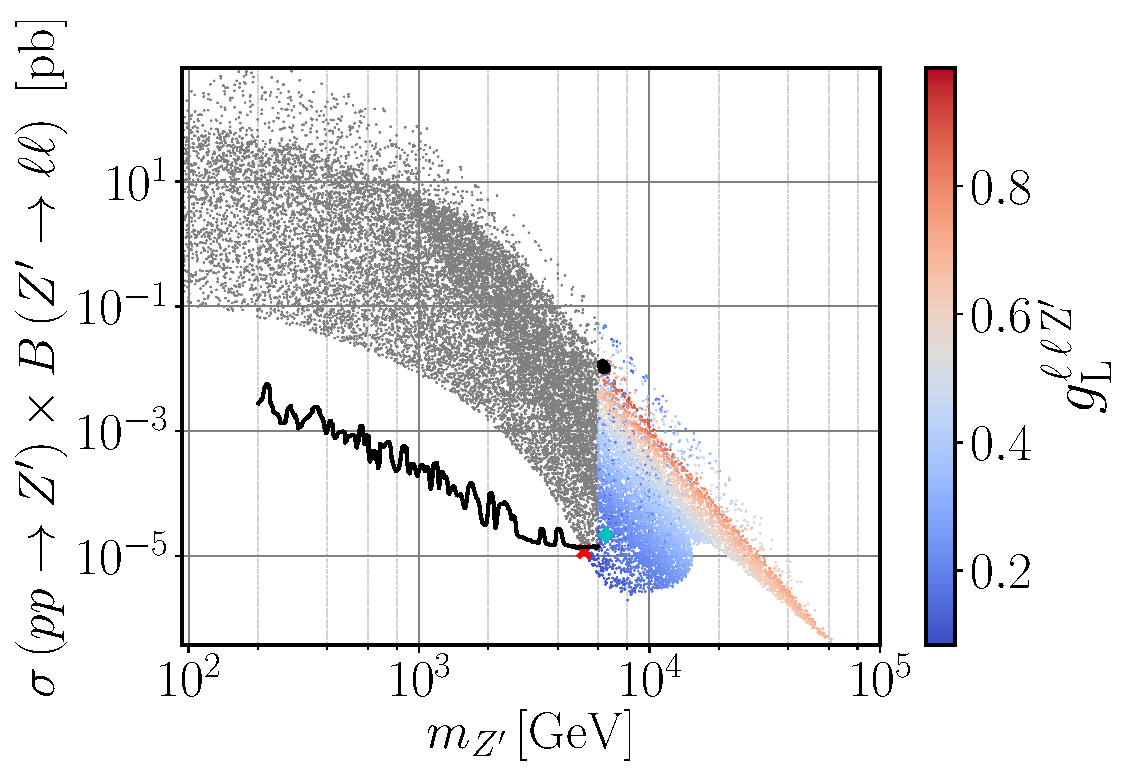
\includegraphics[scale=0.37]{/BLSM/mZp_Xsec_gLmumuZ.pdf}
	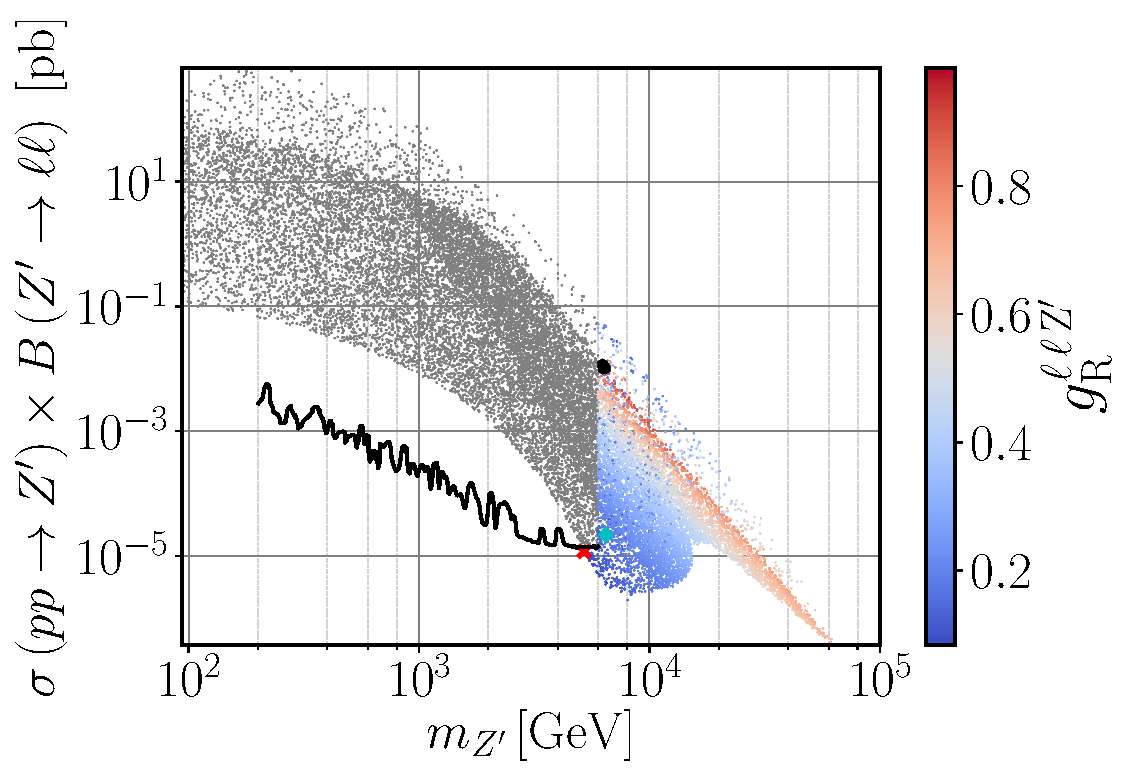
\includegraphics[scale=0.37]{/BLSM/mZp_Xsec_gRmumuZ.pdf}
	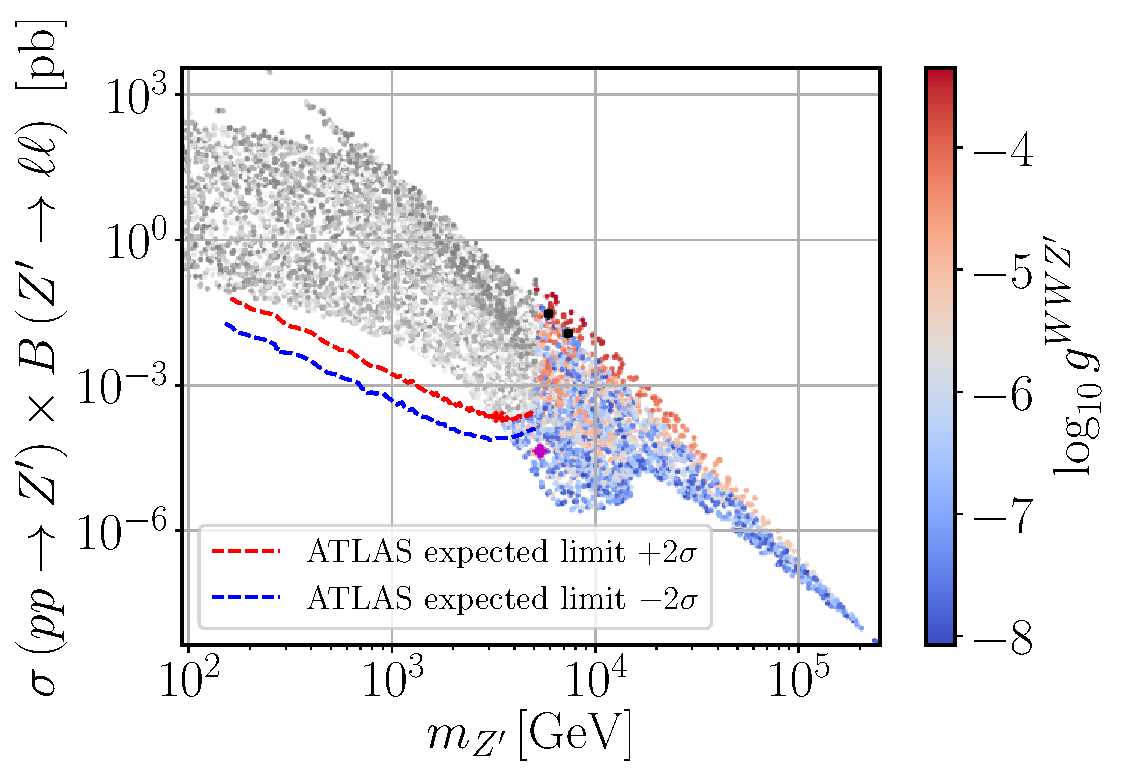
\includegraphics[scale=0.37]{/BLSM/mZp_Xsec_gWWZp.pdf}
	\caption{The same as in Fig.~\ref{fig:Plots4} but with the colour scale representing the coupling of leptons to the $Z^\prime$ (top panels) and the coupling of $W$ bosons to $Z^\prime$.}
	\label{fig:Plots2}
\end{figure}	
%%%%%%%%%%%%%%%%%%%%%%%%%
Note that, for the considered scenarios, the latter can be written as
\begin{equation}
    g^{WWZ^\prime} \simeq \dfrac{1}{16} \dfrac{g_{\ro{YB}}}{g_{\ro{B-L}}} \(\dfrac{v}{x}\)^2\,.
    \label{eq:gWWZp}
\end{equation}
While both $g_{\ro{B-L}}$ and the ratio $v/x$ provide a smooth continuous contribution in the $\sigma B - m_{Z^\prime}$ projection of the parameter space, the observed blurry region in $g^{WWZ^\prime}$ is correlated with the one in the top-left panel of Fig.~\ref{fig:Plots3} as expected from Eq.~\eqref{eq:gWWZp}. On the other hand, the couplings to leptons $g_{\rm L,R}^{\ell \ell Z^\prime}$ exhibit a strong correlation with $g_{\ro{B-L}}$ in Fig.~\ref{fig:Plots3}, in agreement with our discussion above and with Eq.~\eqref{eq:gLgR-simp}. }

\subsection{Barr-Zee type contributions}
\label{sec:BarrZee}

To conclude our analysis, one should note that the two-loop Barr-Zee type diagrams \cite{Barr:1990vd} are always sub-dominant in our case given, that they were not taken into account in the previous calculations. To see this, let us consider the four diagrams shown in Fig.~\ref{fig:Barr-Zee}.
%%%%%%%%%%%%%%%%%%%%%%%%%
\begin{figure}[H]
	\centering
	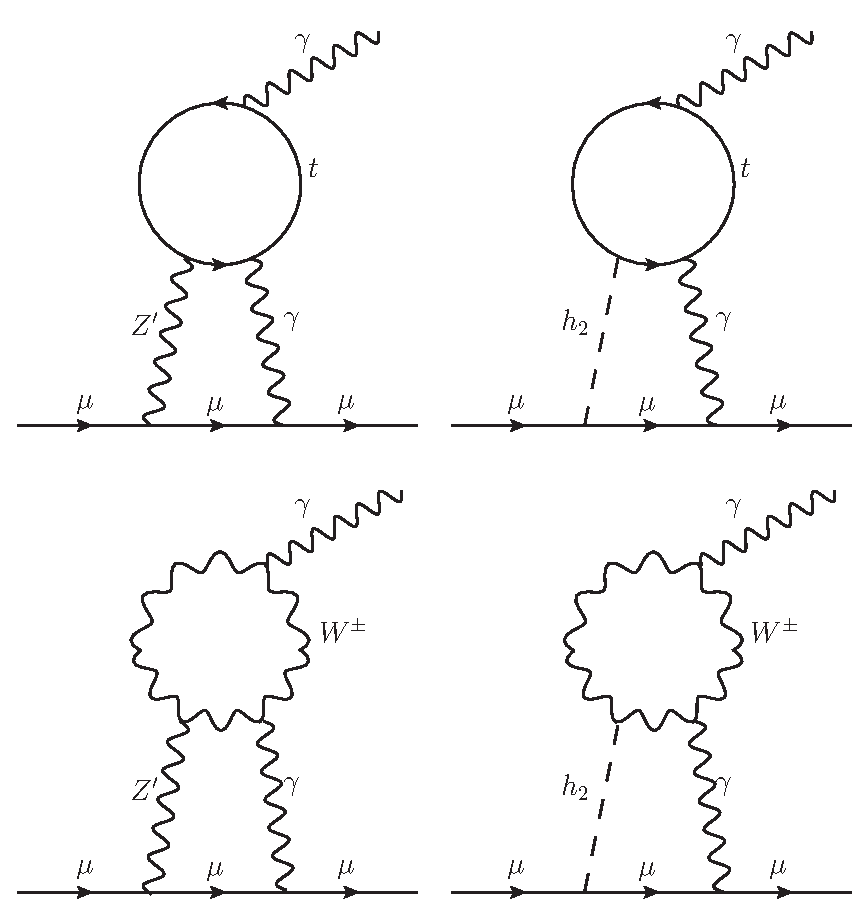
\includegraphics[scale=0.6]{/BLSM/Barr-Zee.pdf}
	\caption{Barr-Zee type two-loop diagrams contributing to $\Delta a_\mu$.}
	\label{fig:Barr-Zee}
\end{figure}	
%%%%%%%%%%%%%%%%%%%%%%%%%
The same reason that suppresses the one-loop $h_2$ contribution in Fig.~\ref{fig:g-2} is also responsible for the suppression of both the top-right and bottom-right diagrams in Fig.~\ref{fig:Barr-Zee} (for details see e.g.~Ref.~\cite{Ilisie:2015tra}). Recall that the coupling of $h_2$ to the SM particles is proportional to the scalar mixing angle $\alpha_h$, which is always small (or very small) as we can see in Fig.~\ref{fig:Plots4}. An analogous effect is present in the diagram involving a $W$-loop, where a vertex proportional to $g^{WWZ^\prime}$ suppresses such a contribution. The only diagram that might play a sizeable role is the top-left one where the couplings of $Z^\prime$ to both muons and top quarks are not negligible.

{ \color{gray}
Let us then estimate the size of the first diagram in Fig.~\ref{fig:Barr-Zee}. This type of diagrams were already calculated in Ref.~\cite{Feng:2009gn} but for the case of a SM $Z$-boson. Since the same topology holds for the considered case of B-L-SM too, 
if we trade $Z$ by the new $Z^\prime$ boson, the contribution to the muon $(g-2)_\mu$ anomaly can be rewritten as
\begin{equation}
    \Delta a_{\mu}^{\gamma Z^\prime} = -\dfrac{g^2 g^2_{\ro{B-L}} m_\mu^2 \tan^2{\theta_W}}{1536 \pi^4} \left( g_{\ro{L}}^{ttZ^\prime} - g_{\ro{R}}^{ttZ^\prime} \right) \ro{T}_7\left( m_{Z^\prime}^2, m_t^2, m_t^2 \right)\,,
    \label{eq:agZ}
\end{equation}
where $T_7$ is a loop integral. % described in appendix \ref{app:T7}. 
%
The parameters $g_{\ro{L,R}}^{ttZ^\prime}$, calculated in \texttt{SARAH}, are the left- and right-chirality projections of the $Z^\prime$ coupling to top-quarks, given by
\begin{equation}
\begin{aligned}
    g_{\ro{L}}^{ttZ^\prime} &= -\dfrac{g_{\ro{B-L}}}{3} \cos{\theta_W^\prime} + \dfrac{g}{2} \cos{\theta_W} \sin{\theta_W^\prime} - \dfrac{g_{\ro{Y}}}{6} \sin{\theta_W} \sin{\theta_W^\prime} - \dfrac{g_{\ro{YB}}}{3} \sin{\theta_W} \sin{\theta_W^\prime}\,,
    \\
    g_{\ro{R}}^{ttZ^\prime} &= -\dfrac{g_{\ro{B-L}}}{3} \cos{\theta_W^\prime} - \dfrac{2 g_{\ro{Y}}}{3} \sin{\theta_W} \sin{\theta_W^\prime} - \dfrac{g_{\ro{YB}}}{3} \sin{\theta_W} \sin{\theta_W^\prime}\,.
\end{aligned}
\end{equation}
The loop integral $\ro{T}_7 \(m_{Z^\prime}^2, m_t^2, m_t^2\)$ was determined in Ref.~\cite{Feng:2009gn} and, in the limit $m_{Z^\prime} \gg m_t$, 
%as we show in Eq.~\eqref{eq:T7-expanded}, 
it can be shown to be simplifiable to, 
\begin{equation}
    \ro{T}_7 \(m_{Z^\prime}^2, m_t^2, m_t^2\) \simeq \frac{2}{m_{Z^\prime}^2} \,,
    \label{eq:T7}
\end{equation}
up to a small truncation error. %(see Appendix~\ref{app:T7} for details).
For the parameter space region under consideration the difference $g_{\ro{L}}^{ttZ^\prime} - g_{\ro{R}}^{ttZ^\prime}$ can be cast in a simplified form as follows 
\begin{equation}
    \left(g_{\ro{L}}^{ttZ^\prime} - g_{\ro{R}}^{ttZ^\prime}\right) \simeq \dfrac{\left(g^2+g_{\ro{Y}}^2\right)g_{\ro{YB}}}{32 g_{\ro{B-L}}} \left(\dfrac{v}{x}\right)^2\,.
    \label{eq:gLminusgR}
\end{equation}
Using this result and the approximate value of the loop factor, we can calculate the ratio between 
the two- and one-loop contributions to the muon $(g-2)_{\mu}$,
\begin{equation}
    \dfrac{\Delta a_{\mu}^{\gamma Z^\prime}}{\Delta a_{\mu}^{Z^\prime}} \simeq -\dfrac{g^2 g_{\ro{Y}^2}}{2048 \pi^2} \dfrac{g_{\ro{YB}}}{g_{\ro{B-L}}} \left( \dfrac{v}{x} \right)^2 \ll 1\,,
\end{equation}
which shows that $\Delta a_\mu^{\gamma Z^\prime}$ does indeed play a subdominant role in our analysis and can be safely neglected. } 



%\chapter{3HDM}
%

\renewcommand{\cleardoublepage}{}
\renewcommand{\clearpage}{}

\chapter{3HDM Model}
\label{ch:3HDM}

We can now move on to the analysis of a three Higgs Doublet Model (3HDM), specifically a minimal BGL-like (Branco-Grimus-Lavoura) 3HDM. 
% 
At the core this BGL treatment is a stabilizing $\mathrm{U}(1) \times \mathrm{Z}_2$ global flavor symmetry, such as presented in Refs.~\cite{Ludvig_Thesis,Ian_Thesis}.
%
Whose purpose is to keep in check flavor violating decays. 
%
Note that without this symmetry these processes would occur at tree-level. 
%
Once the model is properly introduced we continue towards our numerical discussions in a similar fashion as before. 
%
Note, the simulations created for this model used a newer version of the previously discussed code containing the addition of a flavor calculation process based on python3 package entitled \texttt{flavio} \cite{straub2018flavio} and the inclusion of the Higgs alignment limit as to improve the scanning apparatus capabilities and ensure proper gauge couplings to a SM-like Higgs boson.
%
%{ \color{gray} This Higgs alignment process consists in forcing a CP-even eigenstate to serve as the observed Higgs Boson and give it precisely 125.09 GeV mass. This inversion process is achieved trough the translation of all Lagrangian terms relating to the Higgs sector in the gauge basis into physical parameters. } 
%
Note, a key change from the B-L-SM case is that the respective masses will all be calculated at tree-level instead of at 2-loop level. 
%
This is done for multiple reasons most of which reflect computational shortcomings and time constraints.
%
Note that radiative processes are still calculated correctly just using tree-level masses, e.g. the value of $(g-2)_\mu$ is still calculated by SPheno but for a tree-level set of masses.

%{ \color{gray} Our results show that light scalars are still within the reach of future collider experiments in our models framework while having FCNCs concurrent with observations.  
%
%Given these conclusions we also performed a additional as to check if accidental fine-tuning was present in our results, possibly due to a random synchronicity discovered in the Monte-Carlo scan.
%
%To do this we varied all the soft breaking terms for the collected data by 1\% of their original value disregarding the effects this will have for the alignment of the Higgs. 
%
%In the validated parameter space by all other constraints we found no significant sensitivity to mass variation.  
%
%Furthermore for completeness we also implemented a \texttt{MadGraph5\_aMC@NLO 2.6.2} routine as to probe future detection of these light scalars in newer collider experiments and discovered there is still regions that are far from discovery.  \color{blue} maybe conclusions? }  

\section{The Case of the BGL-2HDM and its Relation to our Work}

Any 3HDM can be thought of as part of a larger family of multiple Higgs Doublet Models, or NHDMs, the first iteration of which was the Two Higgs Doublet Model (2HDM) proposed by T.D. Lee \cite{Lee1973}. At the time, Lee was motivated by the search for a spontaneous breaking of the CP symmetry which was included in his model.  However the 2HDM quickly became a very popular model motivated by it's inclusion for dark matter candidates, as well as providing a large particle spectrum, including charged and additional neutral scalars who enable FCNC deviations. In spite of the fact that, now, these tree-level FCNCs are in direct opposition to experimental results, as discussed in section \ref{Chap_1_Sec_3}. Given these limits, we can consult the literature, as in Ref. \cite{Branco:1999fs}, and see that the existence of FCNCs forces the extra scalars in the minimal 2HDM case to have masses above 1 TeV as to suppress FCNCs. These heavy scalars are far from ideal, since there is no indication such heavy scalars exist nor do they provide us with interesting physics. 

Several mechanisms have been proposed to deal with suppression of these tree-level FCNCs as to allow for richer physics and lighter scalars. First, in Ref. \cite{ferreira2019strong}, it is proposed a framework in which we have the balancing of CP-odd and CP-even contribution to FCNCs, however, this requires some fine-tuning, making it very unappealing based on a ``naturalist" argument. Another possibility is to assume alignment between different Yukawa matrices such that no FCNCs are present, see \cite{Jung_2011}. Finally we could also use the approach presented in the BGL version of the 2HDM \cite{Branco_1996}, here the authors impose a flavor-violating symmetry naturally keeping the FCNCs under control trough the CKM matrix. The phenomenology of the model has been studied quite thoroughly in previous works, see Ref. \cite{Botella_2016}, and it remains a possible scenario for BSM physics.

As the name indicates, NHDMs, are types of models where, in parallel with the standard SM Higgs doublet some additional replicas of that same  (or slightly modified) doublet are introduced. In the NHDM these form a sort of family in the scalar sector in analogy to the fermion sector. Being that the 3HDM is the most similar. This idea is far from original and was first discussed by Weinberg in Ref. \cite{Weinberg1976}.

Phenomenologically speaking these 2HDMs and 3HDMs models are quite different however, and we can argue that there are several advantages to the 3HDM. Such as, unlike in the 2HDM case, the 3HDM can provide more than one stable source of spontaneous CP symmetry breaking \cite{Branco_2012}. Furthermore, charge breaking minima were found to be stable while at the same time coexisting with charge-preserving ones (for more information see, \cite{Barroso_2006}). Note also, for the 2HDM a full list of all possible incorporation of symmetries consistent with $\mathrm{SU(2)}\times\mathrm{U(1)}$ has been achieved \cite{Ivanov_2008}, while for the 3HDM no work has thus far been completed, see, \cite{Ivanov_2015}. 

In this work we explore a 3HDM with a global flavor symmetry to replicate the BGL treatment. And in fact similar studies have been done in 3HDMs that include different flavor symmetries, such as Ref.\,\cite{Camargo_Molina_2018}. Given this background it is no surprise that we will focus particularly in the measuring Quark Flavor Violation (QFV) observables. In our analysis these will consist of meson decays or oscillations that include the changing of quark flavor within the meson. These QFV observables will be compared to measured amplitudes in collider experiments as to offer a novel exclusion to our model. Note, the additional flavor symmetry constrains the terms that can appear in the Yukawa sector of the Lagrangian resulting in very specific structures (or textures) of the Yukawa couplings. These shapes generate a suppression mechanism trough the CKM matrix off-diagonal terms restricting the values of FCNCs in our model.%

 
\section{The formulation of a BGL-like 3HDM} 

Again, for this model, we still retain most of the same fields with equal charges as we saw under the $\mathcal{G}_{SM}$ in the SM chapter~\ref{Chap:SM}. These fields are seen in, 
%
\begin{equation}
\label{eq:3HDM_Fields}
\begin{gathered}
Q_{L_i} =  \begin{pmatrix}
u_{L_i}  \\
d_{L_i}
\end{pmatrix} \quad , \quad \Psi_{L_i} =  \begin{pmatrix}
\nu_{L_i}  \\
e_{L_i}
\end{pmatrix}  ,  \\ 
p_R \quad , \quad n_R \quad , \quad e_{R_i} \quad i=\{1,2,3\}  ,  \\  
\phi_k = \begin{pmatrix}
W_k^\pm + i \, W_k^\mp \\ 
\frac{1}{\sqrt{2}}\left( v_k + h_k + i Z_k \right) 
\end{pmatrix}  \quad , \quad k=\{ 1,2,3\}  . 
\end{gathered} 
\end{equation}
%
where $Q_{L_i}$ , $\phi_k$ and $\Psi_{L_i}$ are $\mathrm{SU(2)_L}$ doublets while, $p$ and $n$ (these are analogous to $u_{R_i}$, $d_{R_i}$ in the SM respectively), and $e_{R_i}$ are $\mathrm{SU(2)_L}$ singlets where the i and k generation stand for their respective generation indexes. 
%
Where the new charges under $\mathrm{U(1)}\times\mathbb{Z}_2$ can be seen in the transformations that these fields undergo, 
%
\begin{equation}
\label{eq:3HDM_Transformations}
	\begin{split} 
	\mathrm{U(1)} : & \\
		& Q_{L_3} \rightarrow    e^{i \alpha} Q_{L_3}  \\  
		& p_{R_3} \rightarrow    e^{2 i \alpha} p_{R_3}  \\
		& \phi_1  \rightarrow    e^{i \alpha} \phi_1  \\   
		& \Psi_{L_1} \rightarrow e^{i \alpha} \Psi_{L_1} \\
		& \phi_3 \rightarrow     e^{i \alpha} \phi_3  \\ 
	\end{split} \quad \quad \quad  
	\begin{split}
		\mathbb{Z}_2 : & \\
		 	& Q_{L_3} \rightarrow -Q_{L_3} \\
		 	& p_{R_3} \rightarrow -p_{R_3} \\ 
		 	& \phi_1  \rightarrow -\phi_1 \\ 
		 	& \Psi_{L_1} \rightarrow - \Psi_{L_1} \\ 
		 	& \phi_3 \rightarrow -\phi_3
	\end{split}  
\end{equation} 
%
All remaining fields not shown in Eq. \ref{eq:3HDM_Transformations} remain unchanged under transformations of the $\mathrm{U(1)}\times\mathbb{Z}_2$ global symmetry i.e. are not charged under these symmetries.  
%
Note there is no right handed neutrino fields in this model making it so that no neutrino mass terms appear unlike in the case of the B-L-SM.

\subsection{The Scalar Sector}

Let us then start our proper introduction to the workings of the model by presenting the scalar sector where the new spin-0 $\mathrm{SU(2)}$ doublets, $\phi_k$, $k=\{1,2,3\}$ reside.
%
Note the scalar potential is $\mathcal{CP}$-invariant, this means, 
%
\begin{equation}
\phi_1 = \phi_1^{\**} \quad , \quad \phi_2 = \phi_2^{\**} \quad , \quad 
\phi_3 = \phi_3^{\**} . 
\end{equation}
% { \color{red} Não falta um sinal de menos no $\phi_{1,3}$ Eu disse que o outro não se transforma sobre Z2 mas como isto é CP trans. não devia de ter? Ask morais } 
%
The generic scalar potential is extensively written in, 
\begin{equation}
\label{eq:3HDM_Scalar_Pot}
\begin{split}
V(\phi_i) = & 
- \mu_1^2 \left( \phi^{\dagger}_1 \phi_1 \right) 
- \mu_2^2 \left( \phi^{\dagger}_2 \phi_2 \right)  
- \mu_3^2 \left( \phi^{\dagger}_3 \phi_3 \right) \\ 
& \left[ - \mu_{21}^2 \left( \phi^{\dagger}_2 \phi_1  \right) 
  - \mu_{23}^2 \left( \phi^{\dagger}_2 \phi_3  \right)  
  - \mu_{13}^2 \left( \phi^{\dagger}_1 \phi_3  \right) + \text{H.c.} \right]  \\
& + \lambda_1 \left( \phi^{\dagger}_1 \phi_1 \right) 
  + \lambda_2 \left( \phi^{\dagger}_2 \phi_2 \right)  
  + \lambda_3 \left( \phi^{\dagger}_3 \phi_3 \right) \\  
& + \lambda_4 \left( \phi^{\dagger}_1 \phi_1 \right)  \left( \phi^{\dagger}_2 \phi_2 \right) 
  + \lambda_5 \left( \phi^{\dagger}_1 \phi_1 \right)  \left( \phi^{\dagger}_3 \phi_3 \right)  
  + \lambda_6 \left( \phi^{\dagger}_2 \phi_2 \right)  \left( \phi^{\dagger}_3 \phi_3 \right)  \\ 
& + \lambda_7 \left( \phi^{\dagger}_1 \phi_2 \right)  \left( \phi^{\dagger}_1 \phi_2 \right)  
  + \lambda_8 \left( \phi^{\dagger}_1 \phi_3 \right)  \left( \phi^{\dagger}_3 \phi_1 \right)   
  + \lambda_9 \left( \phi^{\dagger}_2 \phi_3 \right)  \left( \phi^{\dagger}_3 \phi_2 \right)  \\
& + \lambda_{10} \Bigg\{ \left( \phi^{\dagger}_1 \phi_3 \right)^2 + \text{H.c.} \Bigg\} . 
\end{split} 
\end{equation}
%
%{ \color{red} Este potencial tem de ser visto com cuidado. Primeiro, os termos com $\lambda_{1,2,3}$ são iguais aos termos com $\mu^2_{1,2,3}$ mas com o simal trocado. Segundo, porque que é que o $\lambda_{10}$ é o único com Hermıitico conjugado? Não estamos a fazer double counting com isto} 
%
Due to the $\mathcal{CP}$ symmetry imposed on this potential all parameters, $(\lambda_i,i=\{1,...,10\})$ and soft-breaking terms, here are real.
%
The most generic version of this soft breaking is given by the second line, where the soft-breaking terms $\mu_{23}^2$, $\mu_{13}^2$ and $\mu_{21}^2$ are seen. 
%
The parameter $\mu_{23}^2$, is necessarily added as to impede the formation of a massless axion and is the only term that respect the $\mathbb{Z}_2$ symmetry while the others explicitly break it. Note the  $\mathrm{U(1)}$ portion is broken explicitly by all these terms. 
%
%{\color{red} Porque? Todos os termos da segunda linha são genéricos de um potential 3HDM. Não? e porque nao introduzir mais só estes termos quebram a symmetry imposta?} 
%
%Of these note that the $\mu^2_{23}$ term is the only one that respect the $\mathbb{Z}_2$ symmetry while the others also break $\mathrm{U(1)}$ portion. 
%
%A study of these parts of the flavor symmetry, has been included in the first analysis of Ref.~\ref{Ian_Thesis}.

After the process of SBB, all Higgs doublets, $\phi_k$, take a VEV shape similar to that of the SM Higgs, written as, 
%
\begin{equation}
\phi_k = 
\begin{pmatrix}
W_k^\pm + i \, W_k^\mp \\ 
\frac{1}{\sqrt{2}}\left( v_k + h_k + i Z_k \right)
\end{pmatrix}  \rightarrow \langle \phi_k \rangle = \begin{pmatrix}
0 \\ 
\frac{v_k}{\sqrt{2}}
\end{pmatrix} \quad , \quad k=\{ 1,2,3\} .  
\label{eq:3HDM_Higgs_Field_VEV} 
\end{equation} 
%
Here we see the charged portion of the field, $W_k^\pm$, the CP-odd portion, $Z_k$, and finally the CP-even, $h_k$. 
%
%Note that after SBB there will still remain 3 massless states (Goldstone bosons) that will be later absorbed into the gauge bosons $W$ and $Z$. 
%
%This allows for them to be removed from the scalar spectrum.

Recall that, for the given scalar potential $V$ as seen in Eq.\,(\ref{eq:3HDM_Scalar_Pot}) to have a stable vacuum it needs to satisfy the tadpole equations i.e. a unchanging potential ensuring that there is a absolute minimum of energy. 
%
To solve these one must write the derivatives of the potential with respect to the fields and then observe their values once the process of SBB occurs, this process yields the following equations,
%
\begin{equation}
\label{eq:3HDM_tadpoles}
\begin{split}
\frac{\partial V}{\partial \phi_1} = & \frac{1}{2} v_1 \left(-2 \mu _1^2+\left(\lambda _4+\lambda _7\right) v_1^2+\left(\lambda _5+\lambda _8+2 \lambda _{10}\right) v_7^2\right)+\lambda _1 v_1^3-\mu _{13}^2 v_3-\mu _{21}^2 v_2 \\ 
\frac{\partial V}{\partial \phi_2} = & \frac{1}{2} v_2^2 \left(-2 \mu _2^2+\left(\lambda _6+\lambda _9\right) v_3^2+\left(\lambda _4+\lambda _7\right) v_1\right)+\lambda _2 v_2^3-\mu _{21}^2 v_1-\mu _{23}^2 v_3 \\
\frac{\partial V}{\partial \phi_3} = & \frac{1}{2} \left(2 \lambda _3 v_3^3+\left(\lambda _6+\lambda _9\right) v_2^2 v_3+\left(\lambda _5+\lambda _8+2 \lambda _{10}\right) v_1^2 v_3-2 \mu _3^2 v_3-2 \mu _{13}^2 v_1-2 \mu _{23}^2 v_2\right) \\
\end{split} 
\end{equation}

\subsubsection{The Higgs Basis}

It is convenient for the remainder of our study to now introduce the basis changing matrix to what we will call the Higgs Basis.
%
In our analysis of the 3HDM we did not perform the conventional direct diagonalisation of the scalar and Yukawa bi-linear terms expressed in the scalar potential (Eq.\,(\ref{eq:3HDM_Scalar_Pot})) expanded around the vacuum state.
%
Instead we use a intermediate basis in between the process of expressing the mass eigenstates as to significantly simplifies the analysis of the scalar, pseudoscalar, charged scalar and quark physical terms 
%
%Instead of the direct diagonalisation that is often performed of the gauge basis mass forms extracted from the bi-linear terms of the potential see in Eq.\,\ref{eq:3HDM_Scalar_Pot}, expanded around the vacuum state, the use of the intermediate Higgs basis significantly simplifies the analysis of the scalar, pseudoscalar and the charged scalar sectors. 
%
e.g this base change will allow us to express the charge and pseudoscalar states in such a way as to become apparent that a Goldstone emerges in each case. 
%
These Goldstones will account for the longitudinal polarization of W and Z bosons. 

The transformation from the gauge to the Higgs basis reads, 
\begin{equation}
\mathcal{O} = 
\begin{pmatrix}
\dfrac{v}{v_1} & \dfrac{v}{v_2}  & \dfrac{v}{v_3} \\[1.2em]
\dfrac{v_3}{v_{13}} & 0 & \dfrac{-v_1}{v_{13}} \\[1.2em]
\dfrac{v_2 v_1}{v v_{13}}  & \dfrac{v_{13}}{v} & \dfrac{v_2 v_3}{v v_{13}}  
\end{pmatrix} , 
\end{equation}
%
where $v_{13}=\sqrt{v_1^2 + v_3^2}$ and $v=\sqrt{v_1^2 + v_2^2 + v_3^2 }$, the total magnitude. This basis transformation explicitly relate the fields in the following manner, 
%
\begin{equation}
\begin{pmatrix}
\phi_1 \\
\phi_2 \\
\phi_3 \\
\end{pmatrix} = 
\mathcal{O} \begin{pmatrix}
h^\prime \\
H_1^\prime \\
H_2^\prime \\
\end{pmatrix} 
%
\quad , \quad 
%
\begin{pmatrix}
Z_1 \\
Z_2 \\
Z_3 \\
\end{pmatrix} = 
\mathcal{O} \begin{pmatrix}
z \\
A_1^\prime  \\
A_2^\prime  \\
\end{pmatrix} 
%
\quad , \quad 
%
\begin{pmatrix}
W_1^\pm  \\
W_2^\pm  \\
W_3^\pm  \\
\end{pmatrix} = 
\mathcal{O} \begin{pmatrix}
\omega^\pm \\
H_1^{\pm \prime}  \\
H_2^{\pm \prime}  \\
\end{pmatrix} . 
\end{equation}
%
Without accounting for the quark fields. These VEVs can also be parameterized with trough their mixing. 
\begin{equation}
v_1 = v \cos(\psi_1) \cos(\psi_2) \quad , \quad v_2 = v \sin(\psi_1) \cos(\psi_2) \quad , \quad v_3 = v \sin(\psi_2) , 
\end{equation}
%
where the two mixing angles $\psi_1$ and $\psi_2$. 
%
Through this we can re-write the orthogonal mixing matrix, 
%
\begin{equation}
\label{eq:3HDM_Orthg}
\mathcal{O} = 
\begin{pmatrix}
\cos(\psi_1) \cos(\psi_2) & \sin(\psi_2) & \cos(\psi_2) \sin(\psi_1)   \\ 
\cos(\psi_1) & 0 & - \sin(\psi_1)  \\ 
- \sin(\psi_1) \sin(\psi_2) & \cos(\psi_2) &  \cos(\psi_1) \sin(\psi_2)
\end{pmatrix} . 
\end{equation}

%
%This basis also going to form a crucial part of our numerical and theoretical studies, as it's going to be a key component of the the \textit{inversion process}. 
%
%What we mean by this inversion process is simply to write all the terms of the Lagrangian in terms of physical parameters, these are mixing angles and masses. 

%Asides from ensure the proper Gauge boson masses we must also account for the proper Gauge-Higgs interactions. 
%
%We observe Lagrangian terms of the form, 
%
%\begin{equation}
%\frac{g^2 v}{2} W^+_\mu W^{\mu \, -} \left( \frac{1}{v} \sum_{k=1}^3 h_k v_k \right) 
%\end{equation}
%
%We clearly see this to be CP-even Higgs states interacting with the $W^\pm$ bosons, so apriori we must ensure that this represents a physical state relating to the SM Higgs Boson as, 
%\begin{equation}
%h_1 = \left( \frac{1}{v} \sum_{k=1}^3 h_k v_k \right) 
%\end{equation}
%

%This procedure is also called Higgs alignment limit. 
%
%This consists in us forcing a eigenstate of the Gauge base to serve as the direct correspondent observed Higgs Boson, leading to a complete superposition (or alignment) of both physical and gauge eigenstates. 
%
%For a more detailed description of the process see Ref. \cite{Ian_Thesis}.  
%
%Note however, although we use a "perfect alignment" there is room for some of the Higgs boson to be a mixture of other scalar states of this kind (about $\mathcal{O}(10\%)$, as discussed in \ref{Aad_2020}. 

%Given we impose in our work the perfect Higgs aligment we are not scanning all of the available parameter space that can be accessible to the 3HDM. 
% 
%However given our random methodology allowing for mixing would decrease by several orders of magnitude our scans time efficiency. 
%
%Given time investment, a future version of the presented algorithm (possibly made "smarter" trough new techniques applied in the field such as ML {\color{red}{citar Pino ou Felipe}}) could efficiently observe and constrict EW effects coming from a more complex mixture of scalars and find more viable regions of the parameter space.  

\subsection{The Gauge Sector}

Before beginning our study of the inversion process of the scalar sector it is prudent to first consider and discuss the remaining portions of the 3HDM Lagrangian. 
%
We begin this by present first the Gauge sector. 
%
Note, after the Higgs Doublets shift to their VEVs we have the following mass terms, 
%
\begin{equation}
\mathcal{L}_{\text{gauge}} \supset \frac{1}{4} \left( v_1^2 + v_2^2  + v_3^2 \right) g^2 W^+_\mu W^{-\,\mu} + \frac{1}{8} \left(  v_1^2 + v_2^2  + v_3^2  \right) \left( g^{\prime \, 2} + g^2 \right) Z_\mu Z^\mu  .
\end{equation}
%
We can clearly see that to reproduce the correct gauge boson masses we must ensure that,
%
\begin{equation}
\label{eq:VEV_Condition}
\sum_{k=1}^3 v_k^2 \approx 246^2 \ \text{(GeV)}^2  . 
\end{equation}
%
This is a very important condition as it will reflect what range of values that are available for our Higgs Doublets to take.

Recall that additional gauge couplings to the Higgs bosons have also been precisely measured meaning the only way to achieve the correct Higgs kinetic constraints and weak interactions is to a have $h$ state that corresponds to the observed Higgs state with the measured 125.09 GeV mass. 
%
%This requires us to have a physical state that is a direct reproduction of the SM Higgs with 125.09 GeV.
This is why we impose the previously meantioned Higgs aligment limit as otherwise different tree-level couplings to the gauge bosons would show themselves. 
%
This is explicitly demonstrated in Ref.~\cite{das2015implications}. 

This alignment then consists in a particular configuration of the 3HDM parameter space making so that one of the Higgs states in the gauge basis completely overlaps with a physical state i.e completely aligned with the CP-even physical Higgs boson ($h$). 

In the 3HDM this alignment is also conveniently used to reproduce the same SM-like Leptonic Yukawa sector, as couplings and structure remain the same given the leptons couple exclusively to this SM-like Higgs. 
%
This means the 3HDM is lepton flavour universal just like the SM. 

Note that strict alignment is not manifestly required by the data and in fact there are ways we could deviate as much as $\mathcal{O}(10\%)$ (see Ref.\,\cite{Aad_2020}) from the SM predicted gauge coupling value trough light mixing. 

This means we are ignoring some of the parameter space by imposing precise Higgs Aligment.
%
However given our random methodology allowing for mixing would decrease by several orders of magnitude our scans efficiency. 
%
Given time investment, a future version of the presented algorithm (possibly made "smarter" trough new techniques applied in the field such as machine learning) could efficiently observe and constrict EW effects coming from a more complex mixture of scalars and find more viable regions of the parameter space.  

\subsection{The Yukawa sector}

Now having dealt with the scalar and gauge sector we can continue to study the Yukawa sector. 
%
The Yukawa portion of the Lagrangain is seen in,
% Moving onto the Yukawa portion of the Model, we can write the Yukawa sector to be,
% The quark Yukawa Lagrangian for a 3HDM will take the general form, 
\begin{equation} \label{eq:3HDM_Yuk} \begin{split} 
\mathcal{L}_Y = - & \sum_{k=1}^3 \left[ \overline{Q}_{L_a} \left( \Gamma_k \right)_{ab} \sigma_k n_{R_b} + \overline{Q}_{L_a} \left( \Delta_k \right)_{ab} \tilde{\phi}_k p_{R_b} + \text{H.c}.  \right] \\ + & \left( \Psi_{L_a} \left( Y^e_1 \right)_{ab} \phi_1 e_{R_b} + \text{H.c} \right) .
\end{split} \end{equation} 
% The n fields are down 
% The p fields are up 
Here we see the quark and lepton interactions, note that $\Gamma_k$ and $\Delta_k$ are the down and up Yukawa matrices in the 3HDM model respectively, one for each, $k$, generation.
%
Notice how the leptons couple only to the first generation Higgs Doublet. 
%
This translates into the lepton Yukawa matrix being diagonal as in the SM, allowing leptons to couple exclusively to the lightest doublet, $\phi_1$ and preserving lepton flavour universality, 
%
% Making the Yukawa matrix for Leptons to be, 
\begin{equation}
Y^e_1 = \frac{\sqrt{2}}{v_1} M_{\text{diag.}}\left( m_e , m_\mu , m_\tau \right) .
\end{equation} 
%
%Note that there are no neutrino right handed fields, just like in the SM in Eq. \ref{eq:3HDM_Yuk}. 
%
Furthermore, examining the effects the imposed symmetry, $\mathrm{U}(1)\times\mathbb{Z}_2$, had on the at the shape of the Yukawa matrices leads us to discover their texture.  
%
\begin{equation}
\begin{aligned}
&\Gamma_1  = \begin{pmatrix}
0 & 0 & 0\\
0 & 0 & 0\\
\times & \times & 0
\end{pmatrix}, \quad 
&&\Gamma_2  = \begin{pmatrix}
\times & \times & 0\\
\times & \times & 0\\
0 & 0 & 0
\end{pmatrix}, \quad
\Gamma_3  = \begin{pmatrix}
0 & 0 & 0\\
0 & 0 & 0\\
0 & 0 & \times
\end{pmatrix}, \\[1em]
&\Delta_1  = \begin{pmatrix}
0 & 0 & 0\\
0 & 0 & 0\\
0 & 0 & 0
\end{pmatrix}, \quad 
&&\Delta_2 = \begin{pmatrix}
\times & \times & 0\\
\times & \times & 0\\
0 & 0 & 0
\end{pmatrix} , \quad 
\Delta_3 = \begin{pmatrix}
0 & 0 & 0\\
0 & 0 & 0\\
0 & 0 & \times
\end{pmatrix}. 
\end{aligned} 
\end{equation}
%
Note, here the $\times$ represent a complex non-zero value in the respective matrix. 
%
We can immediately see the treatment of the first generation of quarks differ between bottom and up types. 
%
% The zero entries in these matrices are imposed by the $\mathrm{U}(1)\times\mathbb{Z}_2$. 
%
These textures of the Yukawa matrices and the size of their components will determine the strength of FCNCs at tree and loop-levels. 
%
% You can see these Yukawa Matrices include FCNCs at tree level given their non diagonal entries, these FCNCs are suppressed by the CKM matrix. 
%
%In fact we will see the heavy massive eigenstate $H_2$ and $H_3$ mediate these FCNCs, this is a very relevant feature of our model. 
%
The quadratic terms that spawn in the Lagrangian after SBB have the following relations to the Yukawa matrices,
% 
\begin{equation}
\label{eq:3HDM_Quark_gauge_mass}
\begin{split}
M_n = \frac{v_1}{\sqrt{2}} \Gamma_1 +  \frac{v_2}{\sqrt{2}} \Gamma_2 +  \frac{v_3}{\sqrt{2}} \Gamma_3  \quad , \\ 
M_p = \frac{v_1}{\sqrt{2}} \Delta_1 +  \frac{v_2}{\sqrt{2}} \Delta_2 +  \frac{v_3}{\sqrt{2}} \Delta_3   \quad .
\end{split}
\end{equation}
%
Here we begin to see for the first time the origin of the tree-level FCNCs in 3HDMs given the Yukawa textures. We observe the following mass terms in the gauge basis, 
%
%The mass diagonalization of the Yukawa sector is not possible. We observe the following mass matrices, 
\begin{equation}
M_n = \begin{pmatrix}
\times & \times & 0 \\
\times & \times & 0 \\
0 & 0 & \times 
\end{pmatrix} 
\quad , \quad 
M_p=\begin{pmatrix}
\times & \times & 0 \\
\times & \times & 0 \\
\times & \times & \times 
\end{pmatrix} .
\end{equation}
%
Note that there is no overlap between matrix elements inside the up or down sectors, e.g for the case of the $(m_p)_{31}$ and $(m_p)_{32}$ only the first matrix, $\Gamma_1$ contributes for its value, 
\begin{equation}
(M_p)_{31} = \frac{1}{\sqrt{2}} v_1 (\Gamma_1)_{31} \quad , \quad (M_p)_{32} = \frac{1}{\sqrt{2}} v_1 (\Gamma_1)_{32} \quad . 
\end{equation}
%
However, to properly examine this sector we must be able to transform the Lagrangian $n$ and $p$ into their proper quark fields $d$ and $u$ respectively. 
%
This, like in the SM, is achieved by a set of bi-unitarity transformations, $V_{L,R}$ and $U_{L,R}$, that will relate the Gauge basis and the mass basis. Where naturally the CKM matrix will be $V_{\text{CKM}} = V_L^\dagger U_R$. These matrices are defined such, 
%
\begin{equation}
%\begin{split}
M^u = V_L^n M_n V_R^n \approx V_L^n \begin{pmatrix}
\times & \times & 0 \\
\times & \times & 0 \\
0 & 0 & \times 
\end{pmatrix}  V_R^n  \quad , \quad 
m^d = U_L^p  M_p U_R^p \approx U_L^p \begin{pmatrix}
\times & \times & 0 \\
\times & \times & 0 \\
\times & \times & \times \\ \end{pmatrix} U_R^p . 
%\end{split} 
\end{equation}
This then imposes certain shapes to the unitary transformations we apply,
\begin{equation}
V^{p}_{L} = \begin{pmatrix}
\times & \times & 0 \\ 
\times & \times & 0 \\
0 & 0 & 1 \\ 
\end{pmatrix} \quad , \quad   V^{p}_{R} = \begin{pmatrix}
\times & \times & 0 \\ 
\times & \times & 0 \\
0 & 0 & e^{i\alpha}  \\ 
\end{pmatrix}  \quad , \quad 
U^{n}_{L,R} = 
\begin{pmatrix}
\times & \times & \times \\ 
\times & \times & \times \\
\times & \times & \times \\
\end{pmatrix} .
\end{equation}
We introduce a complex phase in $V^p_{L,R}$ so that these matrices can be parametrized with two angles. While the parametrization of $U^n_{L,R}$ will require 3. We know these to be the physical degrees of freedom that will be included in the CKM matrix. The CKM matrix elements can then be expressed as, 
\begin{equation}
\begin{gathered}
V_{CKM} = V_L^p U_R^{n\, \dagger}  \ , \\ 
\\
\begin{pmatrix}
V_{ud} & V_{us} & V_{ub} \\
V_{cd} & V_{cs} & V_{cb} \\ 
V_{td} & V_{ts} & V_{tb} 
\end{pmatrix}  = \begin{pmatrix}
V_{L,11}^p & V_{L,12}^p & 0 \\ 
V_{L,21}^p & V_{L,22}^p & 0 \\ 
0 & 0 & e^{i \alpha} 
\end{pmatrix} \begin{pmatrix}
U_{R,11}^n & U_{R,12}^n & U_{R,13}^n \\
U_{R,21}^n & U_{R,22}^n & U_{R,23}^n \\
U_{R,31}^n & U_{R,32}^n & U_{R,33}^n \\
\end{pmatrix} ^\dagger \ .
\end{gathered} 
\end{equation}
%
While by moving to the mass basis, 
%\begin{equation}
%\begin{split}
%\overline{n}_L m_n \, n_R + \overline{p}_L m_p \, p_R = & 
%\overline{d}_L \left( V_L^n M_n V_R^n \right) d_R + \\ 
%& 
%\end{split} 
%\end{equation}
%
%where the physical quark mass forms and fields are redefined to include the unitarity transformations. 
We can write that $U_L^\dagger = V^\dagger_{\text{CKM}} V_L^\dagger$, which together with,
\begin{equation}
%\begin{split}
M_u^{\text{diag}}  = U_L M_p U_R  \quad , \quad M_d^{\text{diag}}  = V^\dagger_{\text{CKM}} U_L^\dagger M_n U_R \ . 
%\end{split}  
\end{equation} 
%
These equations allow for a system of coupled linear equations that can be solved with respect to the Yukawa textures and return their values for a given set of Unitary matrices, CKM matrix and quark masses. 
%
This portion of the inversion is also performed as we expect to have proper quark masses and to respect the CKM matrix in all our parameter space.
% 
%Although given it's relative simplicity we will not present explicitly it's solutions. 

\section{The BGL-like suppression of FCNCs in the 3HDM model}

Given that we now know how quark and lepton masses are generated in the model and how to express their physical fields let us now analyse carefully the Yukawa couplings between the scalar eigenstates and the physical quarks, with particular attention to any FCNC couplings which may arise as to discuss it's supression.
%
First by performing the discussed shift to the Higgs basis, where $\{\phi_1 , \phi_2 , \phi_3\}$ become $\{h^\prime , H_1^\prime , H_2^\prime \}$ 

In terms of quark field interactions with these states in the gauge basis we have, 
%
\begin{equation}
\mathcal{L}_Y^{\text{CP-even}} = 
- \frac{1}{\sqrt{2}} \left[ \overline{n}_L \left( \sum_{k=1}^3 \Gamma_k \phi_k \right) n_R + \overline{p}_L \left( \sum_{k=1}^3 \Delta_k \phi_k \right) p_R  + \text{H.c.}  \right] . 
\end{equation}
This can be represented in terms of the field $h^\prime$ as, 
\begin{equation}
\mathcal{L}_Y^{H_0} =
- \frac{h^\prime}{v} \left[ \overline{n}_L \left( \sum_{k=1}^3 \Gamma_k v_k \right) n_R + \overline{p}_L \left( \sum_{k=1}^3 \Delta_k v_k \right) p_R + \text{H.c.} \right] .
\end{equation}
%
Where we can replace the result seen in, Eq.\,(\ref{eq:3HDM_Quark_gauge_mass}), 
%
\begin{equation}
\mathcal{L}_Y^{h^\prime} = \frac{h^\prime}{v} \overline{n}_L M_n n_R +  \overline{p}_L M_p p_R .  
\end{equation} 
Showing that the SM like Higgs in our model has the same type of tree-level coupling as in the SM. 
%
Meanwhile for the, generally, heavier states $H_{2,3}^\prime$ we can write their coupling to down quarks as, 
\begin{equation}
\mathcal{L}^{H_1^\prime \, , \, H_2^\prime}_Y = 
\frac{H_1^\prime}{v} \overline{n}_L N_{d\,1} n_R + 
\frac{H_2^\prime}{v} \overline{n}_L N_{d\,2} n_R + 
\text{H.c.} \ . 
\end{equation} 
% 
where the matrix terms $N_{d\,1}$ and $N_{d\,2}$ can be shown to be, 
\begin{equation}
\begin{split}
N_{d\,1} = & \frac{v}{\sqrt{2} v_{13}} U_L^\dagger \left( \Gamma_1 v_3 - \Gamma_3 v_1 \right) \ , \\ 
N_{d\,2} = & U_L^\dagger \left[ \frac{v_2}{v_{13}} \frac{1}{\sqrt{2}} \left( \gamma_1 v_1 + \gamma_3 v_3 \right) - \frac{v_{13}}{v_2} \frac{1}{\sqrt{2}} \Gamma_2 v_2  \right] U_R \ . 
\end{split} 
\end{equation}
To simply the expression of these interaction terms we go back to the textures of the Yukawas, from the block structures presented, and by virtue of our choice to keep the third row of $U_L$ the same as the \text{CKM} matrix, $(U_L)_{3j} = V_{3j}$. There-for by defining the simple projection operator, $P$ as, 
\begin{equation}
P = 
\begin{pmatrix}
0 & 0 & 0 \\ 
0 & 0 & 0 \\ 
0 & 0 & 1 
\end{pmatrix}. 
\end{equation}
We can in the down sector Yukawa matrices write, 
\begin{equation}
\Gamma_3 = (\Gamma_3)_{33} P \quad , \quad \frac{1}{\sqrt{2}}  \left( \Gamma_1 v_3 - \Gamma_3 v_1 \right) =  P M_d \ .  
\end{equation}
Hence, 
\begin{equation}
\begin{split}
(N_{d\,1})_{ij} = & \frac{v v_3}{v_1 v_{13}} V_{3i}^{\**} V_{3j} (M_d)_{jj} - \frac{1}{\sqrt{2}} \frac{v v_{13}}{v_1} ( \Gamma_3 )_{33} V^{\**}_{3i} (U_R)_{3B},  \\ 
(N_{d\,2})_{ij} = & \frac{v_{13}}{v_2} ( M_d )_{jj} \delta_{ij} + \left( \frac{v_{13}}{v_2} + \frac{v_2}{v_{13}} \right) V^{\**}_{3i} V_{3j} (M_d)_{jj}. 
\end{split} 
\end{equation}
%
We can see trough the proper expansion of these terms that all non diagonal terms, (where $j \neq i$) of  $N_{d\,2}$, contain  one CKM matrix term. While for  $N_{d\,1}$ we have two CKM matrix elements. Even given these terms we must suppress the size of the elements in $\Gamma_1$. 

A similar procedure in the up quark sector would reveal that there are no scalar mediated FCNCs at tree level in
the up sector. 
%
This is due to the special structures of the up type Yukawa matrices, we can see $\Delta_1$ is a empty matrix and this prevents FCNCs.

Thus given the magnitude of these CKM matrix terms we can expect our values to naturally be controlled. 

\section{The inversion process}

Over the course of this introduction we alluded to the Higgs alignment and how we expect one of our scalar states must completely overlap with a possible SM like Higgs. 
%
To ensure this we mentioned we must apply the inversion process to our Lagrangian. 
%
To clarify what we mean by inversion process, it should be possible to write all Lagrangian terms with respect to the physical characteristics of the model, such as mixing angles and physical state masses to their Lagrangian terms in the gauge basis. 

We can begin the inversion process by revisiting the tadpole equations, recall that we must ensure the derivatives of the potential, seen in Eqs.\,(\ref{eq:3HDM_tadpoles}), vanish for some value of the spin-0 fields $\phi_i$ , leads us to the so-called tadpole equations of the model. This enables us to express the $\mu_1$, $\mu_2$ and $\mu_3$ as follows, 
%
\begin{equation}
\label{eq:3HDM_Param_1}
\begin{split}
%
\mu _1^2& =\frac{1}{2} \left(2 \lambda _1 v_1^2+\left(\lambda _4+\lambda _7\right) v_2^2+\left(\lambda _5+\lambda _8+2 \lambda _{10}\right) v_3^2-\frac{2 \left(\mu _{13}^2 v_3+\mu _{21}^2
   v_2\right)}{v_1}\right) , \\ 
%
\mu _2^2 & =\frac{1}{2} \left(\left(\lambda _4+\lambda _7\right) v_1^2+2 \lambda _2 v_2^2+\left(\lambda _6+\lambda _9\right) v_3^2-\frac{2 \left(\mu _{21}^2 v_1+\mu _{23}^2 v_3\right)}{v_2}\right)  , \\ 
% 
\mu _3^2 & =\frac{2 \lambda _3 v_3^3+\left(\lambda _6+\lambda _9\right) v_2^2 v_3+\left(\lambda _5+\lambda _8+2 \lambda _{10}\right) v_1^2 v_3-2 \mu _{13}^2 v_1-2 \mu _{23}^2 v_2}{2 v_3} . 
\end{split}  
\end{equation}

\subsection{The CP-odd portion of the scalar sector}

We can now turn our attention now to the physical scalar spectrum of the model. 
%
This potential is explicitly CP invariant given all parameters are real.
%
In fact in this model we expect to find no more sources of CP-violation than in the SM. 

\subsubsection{Pseudoscalar Eigenstates}

Returning to the CP-odd portion of the scalar sector (related to the $Z_k$ degrees of freedom) contains quadratic terms after the process of SBB.  
%
These are easily extracted from the scalar potential in the form, 
%
% of quadratic terms of the $z$ fields once SBB takes place, seen as, 
%
\begin{equation}
V_{\text{shifted}} \supset \left( \begin{array}{ccc} z_1 & z_2 & z_3 \end{array} \right) \frac{M_P^2}{2} \left( \begin{array}{c} z^1 \\ z^2 \\ z^3 \end{array} \right)  , 
\end{equation} 
%
where $M_P^2$ is the $3\times3$ pseudoscalar mass matrix in a non diagonal form, i.e. in the unphysical gauge basis. 
%
It can however be expressed in a block diagonal matrix trough the rotation matrix we introduced in Eq.\,(\ref{eq:3HDM_Orthg}), thus in the Higgs basis our mass matrix would take the shape of, %  and a new orthogonal rotation matrix, $\mathcal{O}^T$,
%
\begin{equation}
B^2_P = \mathcal{O} M_P^2 \mathcal{O}^T = \left( \begin{array}{ccc}
0 & 0 & 0 \\ 
0 & \left( B^2_P \right)_{22} &  \left( B^2_P \right)_{23} \\
0 & \left( B^2_P \right)_{32} &  \left( B^2_P \right)_{33}
\end{array} \right) , 
\end{equation}
%
The line and column of zeroes in this matrix tells us that it has a zero eigenvalue. 
%
This eigenstate, as previously alluded too, will provide a Goldstone. 
%
This is clearly the Goldstone that will become the longitudinal polarization of the $Z$.  
%
%which of course, is the neutral Goldstone boson that the $Z$ gauge boson will later-on "latch-on" to.
%
%Once this degree of freedom "latches-on" to the Z boson it can be safely removed from the scalar sector.
%
The elements of the $B^2_P$ matrix are given by,
\begin{equation}
\label{eq:3HDMP_pseudo_intermedium}
\begin{split}
\left( B^2_P \right)_{22} = & \frac{-2 \lambda _{10} v_2^3 v_3^2 v_1+\mu _{21}^2 v_1^4+\mu _{23}^2 v_3 v_1^3+2 \mu _{21}^2 v_2^2 v_1^2+v_2^3 \left(\mu _{13}^2 v_3+\mu _{21}^2 v_2\right)}{v_1 v_2 \left(v_1^2+v_2^2\right)}  , \\
\\ 
\left( B^2_P \right)_{32} = & \-\frac{v \left(v_1 \left(\mu _{23}^2+2 \lambda _{10} v_2 v_3\right)-\mu _{13}^2 v_2\right)}{v_1^2+v_2^2}  , \\
\\
\left( B^2_P \right)_{33} = & \frac{v^2 \left(2 \lambda _{10} v_3 v_1^2-\mu _{13}^2 v_1-\mu _{23}^2 v_2\right)}{\left(v_1^2+v_2^2\right) v_3} .
\end{split} 
\end{equation}
%
From the above equations we notice that, apart from the three VEVs, only two parameters, $\lambda_{10}$ and $\mu_{23}$, enter in the pseudoscalar mass eigensystem. 
%
From this intermediate basis we can clearly see that in the Higgs basis the pseudoscalar masses mix in such a way that this mixing could easily be paramatrized by a angle, $\gamma_1$, like so,
%
%Given this fact, we can introduce a final orthogonal matrix,
%
%This is for now defined as, 
\begin{equation}
\mathcal{O}_{\gamma_1} = \begin{pmatrix}
1 & 0 & 0 \\
0 & \cos(\gamma_1) & -\sin(\gamma_) \\ 
0 & \sin(\gamma_1) & \cos(\gamma_1) \\
\end{pmatrix} ,
\end{equation}
Therefor the mass eigenstates of the pseudoscalars in the mass basis can be related to the gauge basis by the equation,
\begin{equation}
\label{Rot_1_3HDM}
\mathcal{O}_{\gamma_1} \left( B_P \right)^2 \mathcal{O}_{\gamma_1}^T   = \begin{pmatrix}
0 & 0 & 0 \\ 
0 & m_{A_1} & 0 \\ 
0 & 0 & m_{A_2}
\end{pmatrix} ,
\end{equation}
Expanding the system seen in Eq.\,(\ref{Rot_1_3HDM}), we can deduce the equations for the mass terms in terms of the original Lagrangian parameters, 
\begin{equation}
\label{eq:3HDM_Pseudo_relation}
\begin{gathered}
m_{A_1}^2 \cos ^2\left(\gamma _1\right)+m_{A_2}^2 \sin ^2\left(\gamma _1\right)) = \left( B^2_P \right)_{22}, \\
m_{A_1}^2 \sin \left(\gamma _1\right) \cos \left(\gamma _1\right)+m_{A_2}^2 \sin \left(\gamma _1\right) \cos \left(\gamma _1\right) = \left( B^2_P \right)_{32}, \\ 
m_{A_1}^2 \sin ^2\left(\gamma _1\right)+m_{A_2}^2 \cos ^2\left(\gamma _1\right) = \left( B^2_P \right)_{33}. 
\end{gathered}
\end{equation}
From these two sets of equations (Eq\,(\ref{eq:3HDM_Pseudo_relation}) and Eq.\,(\ref{eq:3HDMP_pseudo_intermedium})) we can show that, % we can show that,
\begin{equation}
\begin{split}
m_{A_1} = \frac{1}{v_1 v_2 \left(v_1^2+v_2^2\right)} \Bigg[ & v v_2 v_1 \tan \left(\gamma _1\right) \left(v_1 \left(\mu _{23}^2+2 \lambda _{10} v_2 v_3\right)-\mu_{13}^2 v_2\right)-2 \lambda _{10} v_2^3 v_3^2 v_1 \\ &  + \mu _{21}^2 v_1^4+\mu _{23}^2 v_3 v_1^3+2 \mu_{21}^2 v_2^2 v_1^2+v_2^3 \left(\mu _{13}^2 v_3+\mu _{21}^2 v_2\right) \Bigg],  \\ 
\end{split}
\end{equation}
%
and 
%
\begin{equation}
\begin{split}
m_{A_2} = \frac{1}{v_1 v_2 \left(v_1^2+v_2^2\right)} \Bigg[ & v v_2 v_1 \cot \left(\gamma _1\right) \left(\mu _{13}^2 v_2-v_1 \left(\mu _{23}^2+2 \lambda _{10} v_2 v_3\right)\right)-2 \lambda_{10} v_2^3 v_3^2 v_1 \\ & +\mu _{21}^2 v_1^4+\mu _{23}^2 v_3 v_1^3+2 \mu_{21}^2 v_2^2 v_1^2+v_2^3 \left(\mu _{13}^2 v_3+\mu _{21}^2 v_2\right) \Bigg].
\end{split} 
\end{equation} 
%
Trough the inversion of these equations we can obtain a parametrization of, $\lambda_{10}$, $v$, trough the mixing angles $\psi_{1,2}$ VEV magnitude, $v$, and the new pseudacalar mixing angles $\gamma_{1,2}$, as seen in,
%
\begin{equation}
\begin{split}
\lambda_{10} = - \frac{1}{2 v_1 v_2^3 v_3^2}  \Bigg[ & v_1^3 \left(\mu_{21}^2 v_1+\mu_{23}^2 v_3 \right) +2 \mu_{21}^2 v_1^2 v_2^2 + \mu_{21}^2 v_2^4 +\mu_{13}^2 v_2^3 v_3 \\ & - v_1 v_2 \left( v_-1^2 + v_2^2 \right) \left(m_{A_1}^2 \cos^2\left(\gamma _1\right)+m_{A_2}^2 \sin ^2\left(\gamma _1\right)\right) \Bigg] \ , \\
\end{split}
\end{equation}
%
\begin{equation}
\begin{split}
\mu_{23} = -\frac{1}{v^2 v_3 \left(v_1^2-v_2^2\right)} \Bigg[  & -v^2 v_1^2 v_2 m_{A_1}^2 \cos ^2\left(\gamma _1\right)+v_2^3 v_3^2 m_{A_1}^2 \sin ^2\left(\gamma _1\right) \\ & - v^2 v_1^2 v_2 m_{A_2}^2 \sin^2\left(\gamma _1\right)  +v_2^3 v_3^2 m_{A_2}^2\cos^2\left(\gamma _1\right)+\mu_{21}^2 v^2 v_1^3 \\ & + \mu_{21}^2 v^2 v_1 v_2^2 \Bigg] \  . 
\end{split}
\end{equation}
Through these two equations we can also express and the final line of Eq.\,(\ref{eq:3HDM_Pseudo_relation}) the $\mu_{21}^2$ soft-breaking term as, 
\begin{equation}
\begin{split} 
\mu_{21}  = \frac{1}{2 v^2 \left(v_1^2+v_2^2\right)} \Bigg[& v_1 v_2 \left(v^2+v_3^2\right) \cos \left(2 \gamma _1\right) \left(m_{A_1}^2-m_{A_2}^2\right) \\ & - v \left(v_1-v_2\right) \left(v_1+v_2\right) v_3 \sin \left(2 \gamma _1\right) 
   \left(m_{A_1}^2-m_{A_2}^2\right) \\ & +v_1 v_2 \left(v-v_3\right) \left(v+v_3\right) \left(m_{A_1}^2+m_{A_2}^2\right) \Bigg] \ .  
\end{split}
\end{equation}
%
This process must be repeated for all the scalar states of the 3HDM as to properly conduct the inversion. 
%
%We will skip some steps in further demostrations since this is just tedius algebriac manipulation while the rational behind the operations remain the same. 

\subsubsection{Charged Scalar Eigenstates}

Through a similar process, we can endeavour to isolate the quadratic terms relating to the charged degrees of freedom. From the charged portion of the Higgs doublets, the $W_\mu$ fields, we express in matrix form the bi-linear terms forming a $M_C^2$ matrix as, 
%
\begin{equation}
V \supset \left( \begin{array}{ccc} 
W_1 & W_2 & W_3 
\end{array} \right) 
\frac{M_C^2}{2} \left( \begin{array}{c}
W_1 \\ 
W_2 \\
W_3
\end{array} \right) \ .
\end{equation}
Trough the same rotation to the Higgs basis we produce a similar structure to the mass matrix of the pseudoscalar fields as seen in,  
%
%For the case of the charged scalars, their mass generation is very similar to the generation of the pseudoscalars where a mass matrix, 
%
\begin{equation}
\label{eq:3HDM_Charged_M1}
B^2_C = \mathcal{O} M_C^2 \mathcal{O}^T = \left( \begin{array}{ccc}
0 & 0 & 0 \\ 
0 & \left( B^2_C \right)_{22} &  \left( B^2_C \right)_{23} \\
0 & \left( B^2_C \right)_{32} &  \left( B^2_C \right)_{33}
\end{array} \right) \ .
\end{equation}
%
Here we observe again that a line and column of zeros ensures that we have a Goldstone boson. Like in the previous example this will be incorporated in the $W^\pm$ Gauge Boson. The terms in this matrix are written as,
%
%In the same fashion as before we define the terms of Eq.\ref{eq:3HDM_Charged_M1}, 
%
%Here we must ensure the same line and column of zeros as to assure we have a goldstone boson that will lead to the mass term of the $W$. In the same fashion as before we can find the equations for all the terms of $B^2_C$ 
%
\begin{equation}
\begin{split}
\left( B^2_C \right)_{22} = & -\frac{1}{2 v_1 v_2 \left(v_1^2+v_2^2\right)} \Bigg[ v_1^3 \left(2 \lambda _7 v_2^3+\lambda _9 v_3^2 v_2-2 \mu _{23}^2 v_3\right)+\lambda _7 v_2 v_1^5+\lambda _7 v_2^5 v_1 \\ & +\left(\lambda _8+2 \lambda _{10}\right) v_2^3 v_3^2 v_1-2 \mu _{21}^2 v_1^4-4 \mu _{21}^2 v_2^2 v_1^2-2 v_2^3 \left(\mu _{13}^2 v_3+\mu _{21}^2 v_2\right) \Bigg] ,  
%
\\
%
\left( B^2_C \right)_{32}  = &  -\frac{v \left(\left(\lambda _8-\lambda _9+2 \lambda _{10}\right) v_1 v_2 v_3-2 \mu _{13}^2 v_2+2 \mu _{23}^2 v_1\right)}{2 \left(v_1^2+v_2^2\right)} \ ,
%
\\
%
\left( B^2_C \right)_{33}  = & \frac{v^2 \left(v_2 \left(\lambda _9 v_2 v_3-2 \mu _{23}^2\right)+\left(\lambda _8+2 \lambda _{10}\right) v_3 v_1^2-2 \mu _{13}^2 v_1\right)}{2 \left(v_1^2+v_2^2\right) v_3} \ . 
%
\end{split} 
\end{equation}
Again we note that given the two final massive eigenstates we can introduce another mixing angle, $\gamma_2$, 
%
\begin{equation}
\mathcal{O}_{\gamma_2} = \begin{pmatrix}
1 & 0 & 0 \\
0 & \cos(\gamma_2) & -\sin(\gamma_2) \\ 
0 & \sin(\gamma_2) & \cos(\gamma_2) \\
\end{pmatrix} \ ,
\end{equation}
Relating to the massive states as, 
\begin{equation}
\mathcal{O}_{\gamma_1} \left( B_C \right)^2 \mathcal{O}_{\gamma_1}^T   = \begin{pmatrix}
0 & 0 & 0 \\ 
0 & M_{H_1^\pm} & 0 \\ 
0 & 0 & M_{H_2^\pm}  
\end{pmatrix} \ .
\end{equation}
%
Where we see the explicit mass eigenstates of the charged scalars $H^\pm_1$ and $H^\pm_2$. 
%
Simple expansion of the equation seen above leads us to the same relations as in the pseudocalar states but now for the charged Higgs states. 
\begin{equation}
\begin{split}
m_{H^\pm_1} \cos^2(\gamma_2) + m_{H^\pm_2}  \sin^2(\gamma_2) = \left( B_C^2 \right)_{22}  \ ,   \\
\cos(\gamma_2)\sin(\gamma_2)( m_{H^\pm_2}^2 - m_{H^\pm_1}^2  )  = \left( B_C^2 \right)_{23} \ , \\ 
m_{H^\pm_1} \sin^2(\gamma_2) + m_{H^\pm_2}  \cos^2(\gamma_2) = \left( B_C^2 \right)_{33} \ . 
\end{split} 
\end{equation}
Notice how the charged eigenstates are dependent only of 3 Lagrangian parameters. For brevety we do not show the mass terms explicitly but given we have three equations we can parameterize another 3 three parameters of the Lagrangian, $\lambda_{7-9}$ in terms of physical masses, VEVs and a mixing angle, as seen, 
\begin{equation}
\begin{split}
\lambda_7 = \frac{1}{v^2 v_1 v_2
   \left(v_1^2+v_2^2\right)} \Bigg[ & -v_1 v_2 \left(v^2+v_3^2\right) \cos \left(2 \gamma _2\right) \left( m_{H^\pm_1}^2 - m_{H^\pm_2}^2 \right) \\ & + \left(v_1-v_2\right) \left(v_1+v_2\right) v_3 v \sin \left(2 \gamma _2\right)
   \left( m_{H^\pm_1}^2  - m_{H^\pm_2}^2 \right) \\ & -v_1 v_2 \left(v-v_3\right) \left(v+v_3\right) \left( m_{H^\pm_1}^2 + m_{H^\pm_2}^2 \right)  \\ & +2 \mu_{21}^2 \left(v_1^2+v_2^2\right) v^2 
   \left( m_{H^\pm_1}^2 - m_{H^\pm_2}^2 \right)  \\ & -v_1 v_2 \left(v-v_3\right) \left(v+v_3\right)  \left( m_{H^\pm_1}^2 + m_{H^\pm_2}^2 \right) \\ & +2 \mu_{21}^2 \left(v_1^2+v_2^2\right) v^2 \Bigg] \ , 
\end{split}
\end{equation}
%
\begin{equation}
\begin{split}
\lambda_8  = \frac{1}{v^2 v_1 v_3} \Bigg[ & 2 \Bigg(\sin \left(\gamma _2\right) m_{\text{C1}}^2 \left(v_1 v_3 \sin \left(\gamma _2\right)-v v_2 \cos \left(\gamma _2\right)\right) \\ & +\cos \left(\gamma _2\right) m_{\text{C2}}^2 \left(v v_2 \sin\left(\gamma _2\right)+v_1 v_3 \cos \left(\gamma _2\right)\right)+v^2 \left(\lambda _{10} v_1 v_3- \mu_{13}^2\right)\Bigg) \Bigg] \ , 
\end{split}
\end{equation}
%
\begin{equation}
\begin{split}
\lambda_9 = \frac{1}{v^2 v_2 v_3} \Bigg[ & 2 \Bigg(-\sin \left(\gamma _2\right) m_{\text{C1}}^2 \left(v_2 v_3 \sin \left(\gamma _2\right)+v v_1 \cos \left(\gamma _2\right)\right)+ \\ & \cos \left(\gamma _2\right) m_{\text{C2}}^2 \left(v v_1 \sin \left(\gamma _2\right)-v_2 v_3 \cos \left(\gamma _2\right)\right)+\mu_{23}^2 v^2\Bigg) \Bigg] \ .
\end{split}
\end{equation} 

\subsection{The CP-even portion of the Scalar Sector}

Finally we can perform the same procedure one final time for the CP-even neutral scalars. 
%Following the same procedure as we did for the CP-odd portion we begin by approaching the quadratic portion of the scalar fields in the potential,
%
Again we begin by rotating the quadratic terms, however this time we require a more complex mixing. In the gauge basis we have,  
\begin{equation}
V \supset \left( \begin{array}{ccc} 
h_1 & h_2 & h_3 
\end{array} \right) 
\frac{M_S^2}{2} \left( \begin{array}{c}
h_1 \\ 
h_2 \\
h_3
\end{array} \right) \ ,  
\end{equation}
%where $M_S^2$ is a $3\times3$ symmetric matrix. 
The elements of this matrix are writen as,

\begin{equation}
M_S^2 = 
\scalebox{0.95}{$
\begin{pmatrix}
 \frac{2 \lambda_1 v_1^3 +\mu_{21}^2 v_2 + \mu_{13}^2 v_3}{v_1} & v_1  v_2 (\lambda_4+\lambda_7)-\mu_{21}^2 & v_1
   v_3 (2 \lambda_{10} + \lambda_5 + \lambda_8) - \mu_{13}^2 \\
 v_1 v_2 ( \lambda_4 +\lambda_7) - \mu_{21}^2 & \frac{\mu_{21}^2 v_1+2 \lambda_2 v_2^3 +\mu_{23}^2 v_3}{v_2} & v_2
   v_3 (\lambda_6+\lambda_9)-\mu_{23}^2 \\
 v_1 v_3 (2 \lambda_{10}+\lambda_5+\lambda_8)-\mu_{13}^2 & v_2 v_3 (\lambda_6+\lambda_9)-\mu_{23}^2 & \frac{\mu_{13}^2 v_1+\mu_{23}^2 v_2 +2 \lambda_3 v_3^3}{v_3} \\
\end{pmatrix}$}.
\end{equation}

%
We must perform a orthogonal rotation such that we reach the scalar mass equations, which is written as, 
%Given the fact that we will have 3 massive eigenstates in this sector with a nontrival mixing we must introduce the following matrices,  
%This matrix has to be diagonalized to reach the massive eigenstates. Moving to the mass basis, $h$, $H_1$ and $H_2$, we use a complementary orgtogonal rotation, $\mathcal{O}_\alpha$,
% The physical CP scalar states that originate from this mass matrix are, , these are obtained trough a orthogonal rotation.
\begin{equation}
\left( 
\begin{array}{ccc}
h & 0 & 0  \\
0 & H_1 & 0 \\
0 & 0 & H_2 
\end{array} 
\right) = \mathcal{O}_\alpha \mathcal{O} \left(M_S^2\right) \mathcal{O}_\alpha^T \mathcal{O}^T \ .
\end{equation} 
However given the non-trivial mixing between these states we define 3 mixing angles $\alpha_{1,2,3}$. Making $\mathcal{O}_\alpha$, 
\begin{equation}
\mathcal{O}_\alpha = R_1 \cdot R_2 \cdot R_3 \quad , 
\end{equation}
which are each written as,
\begin{gather}
R_1 = \begin{pmatrix}
\cos(\alpha_1) & \sin(\alpha_1) & 0 \\
-\sin(\alpha_1) & \cos(\alpha_1) & 0 \\ 
0 & 0 & 1 
\end{pmatrix} \quad , \quad R_2 = \begin{pmatrix}
\cos(\alpha_2) & 0 & \sin(\alpha_2) \\ 
0 & 1 & 0 \\
-\sin(\alpha_2) & 0 & \cos(\alpha_2) 
\end{pmatrix} \quad ,\\ \\ \quad R_3 = \begin{pmatrix}
1 & 0 & 0 \\
0 & \cos(\alpha_3 ) & \sin(\alpha_3) \\
0 & -\sin(\alpha_3) & \cos(\alpha_3) 
\end{pmatrix} \quad . 
\end{gather}
Through this $\mathcal{O}_\alpha$ we can diagonalize scalar massive eigenstates. 
\begin{equation}
\mathcal{O}_\alpha \underbrace{\mathcal{O} M^2_S \mathcal{O}^T }_{B_S^2} \mathcal{O}_\alpha^T \equiv \text{diag}(m_h,m_{H_1},m_{H_2}) \ . 
\end{equation}
Here we can perform another inversion, allowing us to reach a parametrization of the six remaining couplings again trough a laborious expansion, 
\begin{equation}
\begin{split}
\lambda_1 = \frac{1}{2 v^2 v_1^3 \left(v_1^2+v_2^2\right)} \Bigg[ & \left(v_1^2+v_2^2\right) v_1^3 m_h^2+v_1 m_{H_1}^2 \left(v_1 v_3 \sin (\alpha_3)+v v_2 \cos (\alpha_3)\right){}^2 \\ & + v_1 m_{H_2}^2 \left(v v_2 \sin(\alpha_3)-v_1 v_3 \cos (\alpha_3)\right){}^2 \\ & -v^2 \left(v_1^2+v_2^2\right) \left(\mu_{13}^2 v_3+\mu_{21}^2 v_2 \right) \Bigg] \ ,
\end{split} 
\end{equation}
%
\begin{equation}
\begin{split}
\lambda_2 = \frac{1}{2 v^2 v_2^3 \left(v_1^2+v_2^2\right)} \Bigg[ & \left(v_1^2+v_2^2\right) v_2^3 m_h^2+v_2 m_{H_1}^2 \left(v v_1 \cos (\alpha_3) - v_2 v_3 \sin (\alpha_3)\right){}^2 \\ & +v_2 m_{H_2}^2 \left(v v_1 \sin (\alpha_3)+v_2 v_3 \cos (\alpha_3)\right){}^2 \\ & -v^2 \left(v_1^2+v_2^2\right) \left(\mu_{21}^2 v_1+\mu_{23}^2 v_3\right) \Bigg] 
\end{split} \ , 
\end{equation}
%
\begin{equation}
\begin{split}
\lambda_3  = \frac{1}{2 v^2 v_2^3 \left(v_1^2+v_2^2\right)} \Bigg[ & \left(v_1^2+v_2^2\right) v_2^3 m_h^2+v_2 m_{H_1}^2 \left(v v_1 \cos (\text{$\alpha $3})-v_2 v_3 \sin (\alpha_3)\right){}^2 \\ & +v_2 m_{H_2}^2 \left(v v_1 \sin (\alpha_3)  + v_2 v_3 \cos (\alpha_3)\right){}^2  \\ & - v^2 \left(v_1^2+v_2^2\right) \left(\mu_{21}^2 v_1+\mu_{23}^2 v_3\right) \Bigg]  
\end{split} \ ,
\end{equation}
%
\begin{equation}
\begin{split}
\lambda_4 = \frac{1}{v^2 v_1 v_2 \left(v_1^2+v_2^2\right)} \Bigg[ & v_1 v_2 \left(v_1^2+v_2^2\right) m_h^2 + \left(v_1^2+v_2^2\right) v^2 \left(\mu_{21}^2-\lambda_7 v_1 v_2\right) \\ & -m_{H_1}^2 \left(v_1 v_3 \sin (\alpha_3)+v v_2 \cos (\alpha_3)\right) \left(v v_1 \cos (\alpha_3)  -v_2 v_3 \sin (\alpha_3)\right) \\ & + m_{H_2}^2 \left(v_1 v_3 \cos (\alpha_3)- v v_2 \sin (\alpha_3)\right) \left(v v_1 \sin (\alpha_3)+v_2 v_3 \cos (\alpha_3)\right)   \Bigg] \ , 
\end{split} 
\end{equation}
%
\begin{equation}
\begin{split}
\lambda_5 = \frac{1}{v^2 v_1 v_2 \left(v_1^2+v_2^2\right)} \Bigg[ 
& -m_{H_1}^2 \left(v_1 v_3 \sin (\alpha_3) + v v_2 \cos (\alpha_3)\right) \left(v v_1 \cos (\alpha_3)-v_2 v_3  \sin (\alpha_3)\right) \\ & + m_{H_2}^2 \left(v_1 v_3 \cos (\alpha_3)  -v v_2 \sin (\alpha_3)\right) \left(v v_1 \sin (\alpha_3) + v_2 v_3 \cos (\alpha_3)\right) \\ & +\left(v_1^2+v_2^2\right) v^2 \left(\mu_{21}^2-\lambda_7 v_1 v_2\right) + v_1 v_2 \left(v_1^2+v_2^2\right) m_h^2 \Bigg]  \ , 
\end{split} 
\end{equation}
%
\begin{equation}
\begin{split}
\lambda_6 = \frac{1}{v^2 v_1 v_2 \left(v_1^2+v_2^2\right)} \Bigg[ &- m_{H_1}^2 \left(v_1 v_3 \sin (\alpha_3)+v v_2 \cos (\alpha_3)\right) \left(v v_1 \cos (\alpha_3)-v_2 v_3 \sin (\alpha_3)\right)  \\ & +  m_{H_2}^2 \left(v_1 v_3 \cos (\alpha_3) -v v_2 \sin (\alpha_3)\right) \left(v v_1 \sin (\alpha_3)+v_2 v_3 \cos (\alpha_3)\right) \\ & +\left(v_1^2+v_2^2\right) v^2 \left(\mu_{21}^2-\lambda_7 v_1 v_2\right) + v_1 v_2 \left(v_1^2+v_2^2\right) m_h^2- \Bigg] \ . 
\end{split} 
\end{equation}
%
The final $\mu_{13}$ soft-breaking term is calculated with the Higgs alignment condition. 

To recapitulate, we can now express the 15 out of 16 Lagrangian terms trough constants. 
%
First using tadpole equations to reach $\mu_{1}^2$ , $\mu_{2}^2$ and $\mu_{3}^2$ in relation to the three VEVs. Secondly $\mu_{23}^2$, $\mu_{21}^2$ and $\lambda_{10}$, can be exchanged for $m_{A_1}$, $m_{A_2}$ and $\gamma_1$. 
%
The remaining nine quartic couplings can be expressed by the five physical masses (three CP-even scalars, and two charged scalars) and four mixing angles (three in the CP-even sector and one in the charged scalar sector). 

In all these relations will impose the strict alignment limit condition. This translates in the lightest scalar state $m_h$ equal to $125.09$ GeV.
%
% This forces all interactions of the lightest scalar $h_1$ to be exactly like that of the SM, ensure it's interactions with the $W$ and $Z$ boson remain the same i.e. the $h_1$ field completely overlaps with $h$ and $H_1$ and $H_2$ are a ortogonal mix of the fields $h_2$ and $h_3$. 

Through this parameterization we can \textit{a priori} ensure a positively defined set scalar states i.e. no tachyonic states as well as account for unboundness from bellow in our numerical scans. 

Likewise, in the quark sector, it is possible to for a set of VEVs determine before hand the tree-level physical masses for quarks and their proper mixing parameters as to respect the CKM matrix. 
%
This inversion will also be key as to ensure we have points in our scans that are all in accordance with quark physics. 

\section{Numerical Discussion of the 3HDM} 

Finally we move to discuss the results of our study of the 3HDM parameter space.
%
%Before we dive into the results, let's review why we discussed during the previous sections the relations between the Lagrangian and the physical parameters. 
%
As stated, at the starting point of our numerical scans we must ensure a positively defined spectrum i.e. no tachyonic solutions and a stable vacuum (at least at tree-level) trough tadpole equations. % from the very beggining.  
% 
% This requirement comes from the sheer number of dimensions we are scanning over with a simple Monte-Carlo method (16 physical parameters).
% 
Then to obtain relevant data in a timely fashion we performed a inversion process as to scan over physical parameters instead of Lagrangian terms.  
% 
This is a fundamental component of our numerical scan and is performed by solving analytical solutions of the equations we discussed previously. 
%
%The system has been analytically solved for $\lambda_{1,10}$, $\mu^2_{1,2,3}$, $\mu_{13}^2$, $\mu_{21}^2$ and $\mu_{23}^2$ with respect to $\psi_{1,2}$, $\alpha_{1,2,3}$ and the VEVs $v_{1,2,3}$.
%
Note, again that we calculate all masses at the inversion stage and SPheno level at tree-level.  

Never the less we must take into account the real radiatively corrected bounds during our analysis. 
%
Although SPheno utilizes tree-level masses for all radiative processes ( like EW observables) and calculates them correctly just with tree-level masses replaced for loop-level masses, it is still relevant to admit that we must consider that the radiative corrections are subdominant as for our results to have any significant validity.
%
Furthermore, considering the amount of data we gathered, even if we make the assumption that a small portion of our results would be discarded given one-loop or higher order corrections to the mass spectrum our conclusions should still hold since there is room to account for deviations in the mass ranges found.
% 
The exercise of proper inversion for higher orders is left for future work.

The ranges of accepted values within our scans are seen in,
%
\begin{table}[H]
\centering
\begin{tabular}{ccc}
$\psi_{1,2} \ ; \ \beta_{1,2} \ ;\  \alpha_{1,2,3}$ & $\|\mu_{23}\|$ , $\|\mu_{21}\|$ , $\|\mu_{13}\|$ &  $m_{A_{1,2}}$,$m_{H_{1,2}^\pm}$,$m_{H_{1,2}}$ \\ \hline
$0- 2\pi$    & $1 \ \text{GeV} - 10 \ \text{TeV}$ & $1 \ \text{GeV} - 11 \ \text{TeV}$   
\end{tabular}
\end{table}

Recall that we included a inversion process in the Yukawa sector as to reproduce the proper fermion masses. 
% 
This required another set of linear equations to be solved, within experimental error bars of all quark and lepton masses.
% 
This also respects the additional constraint that in the particular case of quark mixing we must ensure the proper values of the CKM mixing matrix.  
%
Only once a point is found to be within the desired Lagrangian space while also respecting the conditions for the quark masses, CKM matrix and bound from bellow is it then fed into SPheno and stored. 
%The later of which, the physical paramaters, are what we randomly generate. 
%
\subsection{Methodology and Constraints}

The  methodology used in this analysis of the 3HDM is very similar to the one introduced in the B-L-SM discussion, with two new additions - first the discussed inversion as to assure Higgs alignment - secondly the use of the python3 package called \texttt{flavio}  \cite{straub2018flavio}. 
%
Introduced to enable our simulations to use the existence of quark flavour violation (QFV) processes to constrict our parameter space trough the Wilson coefficients calculated by SPheno. 

These QFV observables will be represented as fractions between the expected SM value and the calculated value for the point that includes the novel NP contributions. 
%
We calculated a large number of flavour violating processes in this fashion, in fact, 31 fractions between expected QFV processses in the 3HDM and the expected theoretical value of the SM were calculated. 
%
%All but a few had very SM like behavior. 

We will avoid a in-depth discussion of how these QFV processes are calculated seeing that for our purposes knowing that their integrated trough functions dependent on Wilson coefficients will suffice. %{\color{red} I want to rephrase or remove this. I should also cite how to calculate these FCNCs, peskin? which chapter? Não queria escrever formulas hamiltonianas aqui. } 

We will however, make the observations that given the additional scalars, in particular the charged scalars, allows for additional Feynman diagram one must consider in addition to the normal loop-level sources of FCNCs and FCCCs in the SM. 
% 
%In fact we start from the assumption that flavour experimental data imposes stringent constraints on the parameter space of our model. 
%
%{ \color{gray} However note that it is not the most stringent later on. } 

\subsubsection{QFV Observables}

In this work we tested the following B, D and K meson channels, being that for the B meson we tested, 
$\mathcal{BR} \left( \rightarrow \chi_s \gamma \right)$, 
$\mathcal{BR} \left( B_0 \rightarrow \ell \bar{\ell} \right)$, 
$\mathcal{BR} \left( B_s \rightarrow \ell \bar{\ell} \right)$, 
$\Delta M_{B_s}$, 
$\Delta M_{B_0}$, 
$\mathcal{BR} \left( B^+ \rightarrow K^+\nu\bar{\nu} \right)$ , 
$\mathcal{BR} \left( B^+ \rightarrow \pi^+\nu\bar{\nu} \right)$, 
$\mathcal{BR} \left( B^0 \rightarrow K^0\nu\bar{\nu} \right)$,  
$\mathcal{BR} \left( B^0 \rightarrow \pi^0 \nu\bar{\nu} \right)$, 
$\mathcal{BR} \left( B^+ \rightarrow \pi^+\nu\bar{\nu} \right)$ , 
$\mathcal{BR} \left( B^+ \rightarrow \ell \nu \right)$ and
$\mathcal{BR} \left( B^+ \rightarrow D \bar{\ell} \bar{\nu} \right)$. 
%
As for the K meson channels we looked into the $\mathcal{BR} \left( K_L \rightarrow \mu \bar{\mu} \right)$,  $\mathcal{BR} \left( K_L \rightarrow \bar{e} e \right)$,  $\mathcal{BR} \left( K^+ \rightarrow \pi^+ \bar{\nu} \nu \right)$, $\mathcal{BR} \left( K_L \rightarrow \pi^0 \bar{\nu} \nu \right)$, $\epsilon_K$ and $\epsilon^\prime/\epsilon$. 
%
Finally for the D meson we tested only $\mathcal{BR} ( D^+ \rightarrow \bar{\ell} \nu ) $

Note that many of these decays are present at tree-level (mediated by the $W^\pm$ e.g. as $B \rightarrow \tau \nu$) and in loop-order (mediated by the Higgs) in the SM. 
%
In fact what we expected to find is a light enhancement of processes already included in the SM trough the exotic additions of scalars along side the suppression mechanisms we discussed above. 

From this large set of QFV observables we present only the ones that show interesting correlations with the parameters of our model and deviate from SM values in any significant way.
%
Specifically these are, $B \rightarrow \chi_s \gamma$, $B_s \rightarrow \mu \mu$, $\Delta M_s$ , $\Delta M_d$ and $\Delta \varepsilon_K$. 
%
Here $\Delta M_s$ and $\Delta M_d$ represent the frequencies for ${B_0}_s - {B_0}_s$ and ${B_0}_d - {B_0}_s$ oscillations respectively. 
 
Given that we present these results in the form Experimental versus SM fractions we can define 1 and 2 sigma error bars for each channel trough the relation, 
%
%Given the fact we aim to present a simulation of a experimental value and the fact we will be presenting our results as fractions of the SM expected value we can define the error bars of each decay trough the experession, 
%
\begin{equation}
E_r = \frac{\text{Exp}_{BR}}{\text{SM}_{BR}} \times \left( \sqrt{\frac{\text{SM}_{error}}{\text{SM}_{BR}}}\right)^2 + \left( \frac{\text{Exp}_{error}}{\text{Exp}_{BR}} \right)^2 \ , 
\end{equation} 
%
where $\text{Exp}_{BR}$ and $\text{Exp}_{error}$ stand for the experimentally measured central value for a given QFV observable and it's experimental error respectively, while the $\text{SM}_{BR}$ and $\text{SM}_{error}$ stands for the QFV predicted theoretical value for the SM and it's theoretical uncertainty respectively. 

For the most relevant observables the following table shows experimental values and error bars along with SM predicted values and theoretical uncertainties, 
%
\begin{table}[H]
\centering
\begin{tabular}{l|cccc}
 Channel & $\text{SM}_{BR}$         & $\text{SM}_{error}$ & $\text{Exp}_{BR}$ & $\text{Exp}_{error}$   \\ \cline{1-5} 
$\mathcal{BR} ( B \rightarrow \chi_s \gamma )$ & 3.29e-4 & 1.87e-05 & 3.32e-4 & 0.16e-4 \\
$\mathcal{BR} ( B_s \rightarrow \mu \mu ) $ & 3.66e-09 & 1.66e-10 & 2.8e-9 & 0.06e-9       \\
$\mathcal{BR} (B_0 \rightarrow  \mu \mu )$ & 1.14e-10 & 1.186e-11 & 0.39e-9    & 0.14e-9       \\
$\Delta M_s$ & 3.97e-13 & 5.07e-14 & 3.334e-13  &  0.013e-13  \\
$\Delta M_d $ & 1.24e-11 & 7.08e-13 & 1.1688e-11 &  0.0014e-11  \\
$\mathcal{BR} (\Delta \varepsilon_K )$ & 1.81e-3  & 2.00e-4 & 2.228e-3  & 0.011e-3     
\end{tabular}
\caption{Table containing SM theoretical uncertainties and values along side with the QFV experimental error bars and 95\% C.L central value as reference \cite{Tanabashi2018}. }
\end{table}

To briefly introduce how these QFV observables relate to NP we show some representative diagrams, as shown in Figs.\,\ref{3HDM_Leptonics}, \ref{fig:3HDM_oscilation_meson} and \ref{fig:3HDMChiSGamma}. Tree-level processes that include $H^\pm_{1,2}$ lead to leptonic and semileptonic (a decay in which one lepton and the corresponding neutrino is produced in addition to one or more hadrons) processes,  
%
\begin{figure}[H]
\centering
\vspace{0.2cm}
\hspace{-1.5cm}
    \subfloat{\begin{fmffile}{Tree-Level-Hmaismenos-1}
              \begin{fmfgraph*}(130,55)
              \fmfleft{i1,B,i2}
              \fmfright{o1,o2}
              \fmf{fermion}{i1,v1}
              \fmf{fermion}{v1,i2}
              \fmfv{l.d=-36,l.a=62,l={$\text{M}$\mylbrace{66}{0}}}{B}
              \fmf{dashes,label=$H^{\pm}$,label.side=left,tension=1.5}{v1,v2}
              \fmf{fermion}{v2,o1}
              \fmflabel{$\ell^- \comma \nu_\ell$}{o1}
              \fmf{fermion}{o2,v2}
              \fmflabel{$\bar{\nu}_\ell \comma \ell^+$}{o2}
              \end{fmfgraph*}
              \end{fmffile}
              }
    \hspace{2cm}
    \subfloat{\begin{fmffile}{Tree-Level-Hmaismenos-2}
		      \begin{fmfgraph*}(120,80)
        	  \fmfset{arrow_len}{10}
	          \fmfstraight
	          \fmfleft{i3,B1,i1}
	          \fmfright{o3,B2,o2,o1}
	          \fmflabel{$\ell^{-} \comma \nu_\ell$}{o1}
	          \fmflabel{$\bar{\nu}_\ell \comma \ell^{+}$}{o2}
	          \fmf{phantom}{i1,v1,o1}
	          \fmf{fermion,tension=0}{o2,v1,o1}
	          \fmf{dashes,label=$H^{\pm}$}{v3,v1}
        	  \fmf{phantom}{i3,v3,o3} 
	          \fmffreeze
  	          \fmfshift{45 down}{B1}
	          \fmfovalblob{.4w}{.5}{B1}
	          \fmfv{l.d=20,l.a=180,l=$\text{M}$}{B1}
	          \fmfshift{30 down}{B2}
	          \fmfovalblob{.4w}{.5}{B2}
	          \fmfv{l.d=-30,l.a=180,l=$\bar{\text{M}}$}{B2}
	          \quark{qai}{}{0.0 ,1.0 }{1.00,infinity}{0,  0}{left} {0, 0}{0,0}{i3,v3}
	          \quark{qci}{}{0.08,1.0 }{1.02,1}       {0,-18}{-left} {0,-6}{0,0}{i3,v3}	
	          \quark{qao}{}{0.0 ,1.0 }{1.00,infinity}{0,  0}{right}{0, 0}{0,0}{v3,o3}
	          \quark{qco}{}{0.0 ,0.92}{0.84,1}       {0,-18}{-right}{0,-6}{0,0}{v3,o3}
              \end{fmfgraph*}
\end{fmffile}}
\vspace{0.9cm}
\caption{Leptonic and semi-leptonic $H^\pm$ tree-level diagrams where M stands for a generic meson. $\ell$ is any lepton with $\nu_\ell$ being the corresponding neutrino.}
\label{3HDM_Leptonics}
\end{figure}
%
%where  $\ell$ is any lepton. 
Again, note that our model is lepton flavour universal, meaning that all generations are included in these diagrams and the neutrino always corresponds to the same lepton generation. 
%Note that in our model is lepton flavour universal so 
%
In Fig\,\ref{3HDM_Leptonics} we see how a virtual $H^\pm$ leads to  meson decay into leptons. 
%
These processes are present in tree-level at the SM.   
%
As for the new neutral Higgs $H_{1,2}$ and pseudoscalars $A_{1,2}$ their processes compete with loop-level processes at the SM. The most relevant include oscillations and rare neutral meson to lepton decays. 
%
\begin{figure}[H]
\centering
    \begin{fmffile}{Meson_oscillation}
	\begin{fmfgraph*}(160,75)
	\fmfleft{i1,B1,i2}
	\fmfright{o1,B2,o2}
	\fmf{fermion}{i1,v1}
	\fmf{fermion}{v1,i2}
    \fmfshift{0 down}{B1}
  	\fmfshift{12 right}{B1}
    \fmfovalblob{.48w}{.4}{B1} 
    \fmfv{l.d=20,l.a=180,l=$\text{M}$}{B1}
    \fmfshift{0 down}{B2}
    \fmfshift{-12 right}{B2}
    \fmfovalblob{.48w}{.4}{B2}
    \fmfv{l.d=-30,l.a=180,l=$\bar{\text{M}}$}{B2}
	\fmf{dashes,label=$H$,label.side=right,tension=1.5}{v1,v2}
	\fmf{fermion}{v2,o1}
	\fmf{fermion}{o2,v2}
	\end{fmfgraph*}
\end{fmffile}
    \caption{Meson oscillation mediated by a neutral scalar Higgs.}
    \label{fig:3HDM_oscilation_meson}
\end{figure}
%
Still at loop-level, we have the final channel, $\chi_s \gamma$. The quark level transition occurring here is, $b \rightarrow s \gamma$ trough the annihilation of a quark and anti-quark. We show the Feynman diagrams where this process happen in Fig. \ref{fig:3HDMChiSGamma},
%

\begin{figure}[H]
\centering
\vspace{0.3cm}
            \subfloat{\begin{fmffile}{feyngraph_3HDM_11}            \setlength{\unitlength}{.04cm}
            \parbox{80pt}{
	        \begin{fmfgraph*}(85,65)
	        \fmfleft{i1,i2}
	        \fmfright{o1}
	        \fmf{fermion,tension=1.9}{i2,v2}
	        \fmflabel{$b$}{i2}
	        \fmf{fermion,tension=1.9}{v1,i1}
	        \fmflabel{$\bar{s}$}{i1}
         	\fmf{dashes,label=$H^-$,label.side=left}{v1,v2}
         	\fmf{fermion,tension=1.1,label=$\bar{u}_i$,label.side=left}{u1,v1}
	        \fmf{fermion,tension=1.1,label=$u_i$,label.side=left}{v2,u1}
	        \fmf{photon,tension=1.8}{u1,o1}
	        \fmflabel{$\gamma$}{o1}
	        \end{fmfgraph*}}
            \end{fmffile}
            }
            \hspace{1.3cm}
            \subfloat{\begin{fmffile}{feyngraph_3HDM_12}            \setlength{\unitlength}{.04cm}
            \parbox{80pt}{
	        \begin{fmfgraph*}(85,65)
	        \fmfleft{i1,i2}
	        \fmfright{o1}
	        \fmf{fermion,tension=1.9}{i2,v2}
	        \fmflabel{$b$}{i2}
	        \fmf{fermion,tension=1.9}{v1,i1}
	        \fmflabel{$\bar{s}$}{i1}
         	\fmf{fermion,label=$u_i$,label.side=left}{v1,v2}
         	\fmf{dashes,tension=1.1,label=$H^+$,label.side=right}{v1,u1}
	        \fmf{dashes,tension=1.1,label=$H^-$,label.side=right}{u1,v2}
	        \fmf{photon,tension=1.8}{u1,o1}
	        \fmflabel{$\gamma$}{o1}
	        \end{fmfgraph*}}
            \end{fmffile}
            }
            \hspace{1.3cm}
            \subfloat{\begin{fmffile}{feyngraph_3HDM_13}            \setlength{\unitlength}{.04cm}
            \parbox{80pt}{
	        \begin{fmfgraph*}(85,65)
	        \fmfleft{i1,i2}
	        \fmfright{o1}
	        \fmf{fermion,tension=1.9}{i2,v2}
	        \fmflabel{$b$}{i2}
	        \fmf{fermion,tension=1.9}{v1,i1}
	        \fmflabel{$\bar{s}$}{i1}
         	\fmf{dashes,label=$H$,label.side=left}{v1,v2}
         	\fmf{fermion,tension=1.1,label=$\bar{d}_i$,label.side=left}{u1,v1}
	        \fmf{fermion,tension=1.1,label=$d_i$,label.side=left}{v2,u1}
	        \fmf{photon,tension=1.8}{u1,o1}
	        \fmflabel{$\gamma$}{o1}
	        \end{fmfgraph*}}
            \end{fmffile}
            }\hspace{0.8cm}
\vspace{0.2cm}
\caption{NP contribution to the transition mediated by a charged or neutral Higgs at one-loop order as to contribute to $\mathcal{BR} (B \rightarrow \chi_s \gamma)$ trough $b \rightarrow \bar{s} \gamma$ }
\label{fig:3HDMChiSGamma}
\end{figure}


\subsubsection{Bounded from bellow}

As in the B-L-SM or any other multiscalar BSM theory, special attention must be given to the to a large set of bounds imposed by the scalar content of the Model. 
%
In the 3HDM, looking at Eq.\,(\ref{eq:3HDM_Scalar_Pot}), we can see that it is not a simple process. This check begins by ensuring the couplings seen in Eq.\,(\ref{Unbound_Stage_1}) are positive so that the potential does not tend towards $-\infty$ when the fields become large. 

\begin{equation}
\label{Unbound_Stage_1}
\lambda_1 > 0  \quad , \quad \lambda_2 > 0 \quad , \quad \lambda_3 > 0 \quad , 
\end{equation}
%
To further find the proper conditions we must follow a procedure similar to the one used in the 2HDM \cite{Branco_1996}.
%
By taking two doublets pairs at a time $(i, j)$ to infinity but such that ensuring that $\phi_i^\dagger \phi_j = 0$ (which is easily accomplish-able, if for one doublet the upper components are zero and for the other one the lower components vanish) one obtains a positive value of the potential for any value of the fields if,
%
\begin{equation}
\lambda_4 > -2 \sqrt{\lambda_1 \lambda_2} \quad , \quad \lambda_5 > -2 \sqrt{\lambda_1 \lambda_3} \quad , \quad \lambda_6 > -2 \sqrt{\lambda_2 \lambda_3} \ . 1
\end{equation}
%
We can also adapt the bounded-from-below necessary conditions from ref. \cite{Moretti_2015} (their expressions 21–24), while considering the fact that the potential of that work is different from ours and making the necessary adjustments.
%
This translates into a generalisation of the above conditions, which become
%
\begin{equation}
\begin{gathered}
\lambda_4 > - 2 \sqrt{\lambda_1 \lambda_2} - \text{min}(0,\lambda_7) \quad , \quad  \lambda_5 > -2 \sqrt{\lambda_1 \lambda_3} - \min(0,\lambda_8 - 2\|\lambda_{10}\|)  \\
\lambda_6 > - 2 \sqrt{\lambda_2 \lambda_3} - \min(0,\lambda_9) \quad . 
\end{gathered} 
\end{equation}
%
These conditions eliminate a great deal of parameter space, and though they are not sufficient ones, they should cover most of the parameter space leading to an unbounded-from-below potential.
% 
Additionally the upper perturbatively bound must be enforced, ensuring all scalar couplings $\lambda_{1,10}$ are maintained bellow $4\pi$.

\subsubsection{Unitarity}

As for constraining the unitarity, we again leave the calculation of the scattering amplitudes of scalar-scalar elastic interactions to SPheno. 
%
In multiple Higgs models this is done by the diagonalization of the S-matrix (S for scattering), comprised of all these amplitudes.
%
Once diagonalized, it can be checked for unitarity, and ensure that at high energies we respect the optical theorem.  
%
This could be done manually by following a process like seen in Ref\,\cite{Moretti_2015}, however it is far more convenient to leave this job for SPheno. 

%Finally, a standard constraint on multiscalar models is to verify their compliance with electroweak precision bounds or STU bounds, see Ref\,\cite{Peskin1992} { \color{red} which chapter?}. 
% 
%Models with N Higgs doublets automatically satisfy $\rho = 1$ at tree-level, meaning bounds on the oblique parameter S will be easily satisfied. These parameters are also calculated by SPheno. 

%However we now have the additional constraint coming from our flavour analysis trough the discussed QFV observables. 
%

\subsection{Discussion of results}

The main objective of our work was to design a tool with whom we can probe large and complicated parameter spaces of BSM models as discussed previously. 
%
A more advanced version of the previously implemented process was implemented in this 3HDM model.
%
With it we tried to scam over all relevant free parameter space and would like to present the results of said scan in this chapter. 
%
%The central discussion of the scanning apparatus will focus on the new flavour constrictions and the inversion process.  
%
With it we find the parameter space that not only respects all scalar and EW analysis as implemented on the B-L-SM model, but also keeps all examined QFV observables within the 2 $\sigma$ deviation limit and ensures the proper inversion process. 
% we can take from a random 3HDM scan with flavour as a chief constricting factor. All flavour observables were kept within the 2 $\sigma$ limit.

We already touched on how Higgs physics can be detected on large collider experiments and how flavour can also limit our searches as strong interactions of quarks trough the exotic Higgs could lead to excess quark violation. % forget the additional EW precision observables that also play a key role in excluding large parts of the available paramater space. 
%
\subsubsection{Electroweak precision observables}

The process we undertook here was exactly the same as we performed on the B-L-SM discussed in section \ref{Sec:B-L-SM-EW}. 
%
We can see the S, T and U variables for our parameter space in the Figs \ref{Fig:3HDM_STU}, 
%
\begin{figure}[H]
	\centering
	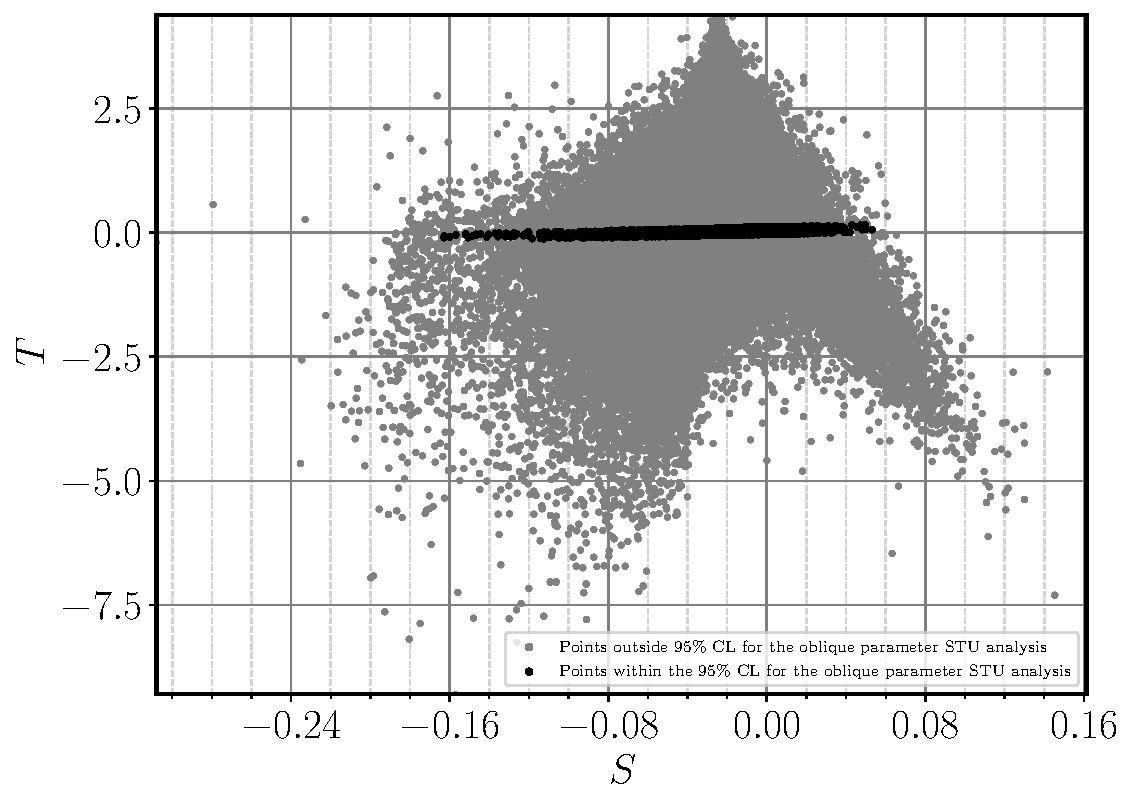
\includegraphics[width=.49\textwidth]{Images/3HDM/EW/EW_S_T_black.pdf}	
	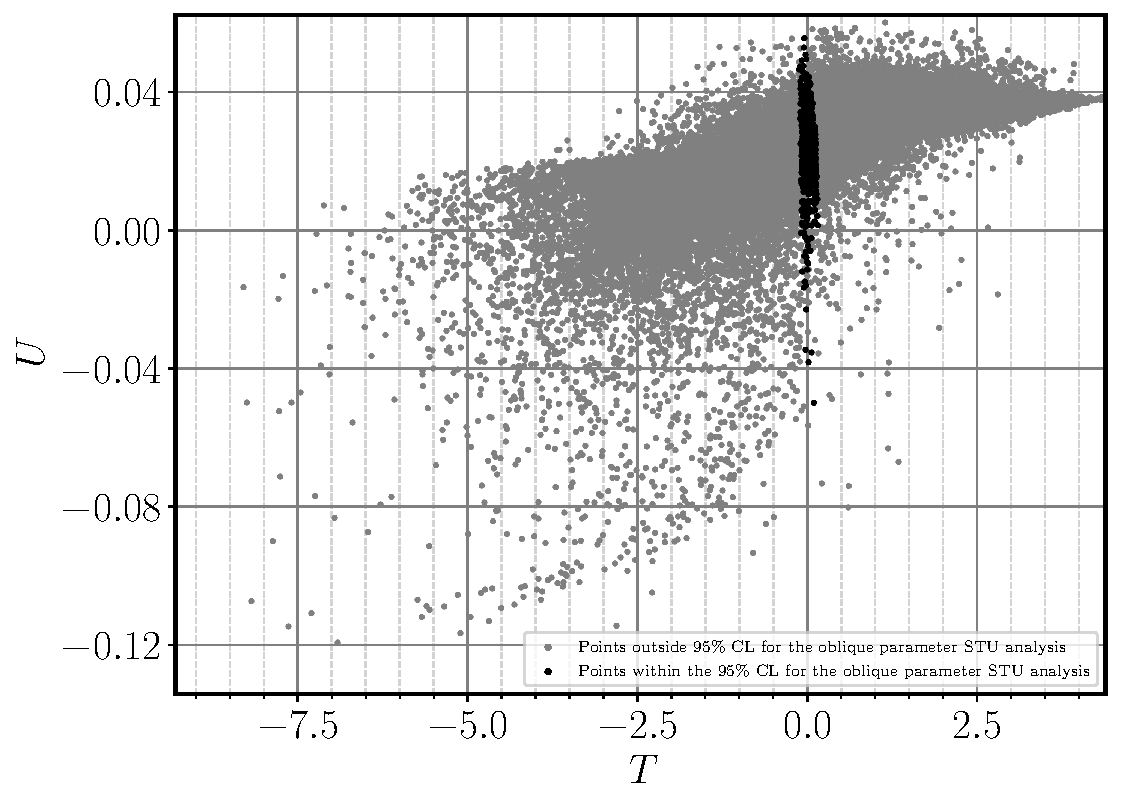
\includegraphics[width=.49\textwidth]{Images/3HDM/EW/EW_T_U_black.pdf}
	\caption{3HDM scatter plots for EW  precision  observables  showing  the ST(left)  and TU(right)planes.  Accepted points lying within a 95\% C.L. ellipsoid of the best fit point are represented inblack whereas grey points are excluded.}
	\label{Fig:3HDM_STU}
\end{figure}
%
We can clearly see that NP can have a very strong effect on some of these observables, most notably in the deviation in the T variable.
%
Note that this wide variation makes the elipsoid seen previously look like a narrow region. 
%
As in the B-L-SM the values for $(\Delta S , \Delta T , \Delta U )$ are taken from \cite{Baak_2012}.

% Meantion :  In order to test the obliqueparameters, we implement results for the SM fit from the Gfitter collaboration [45].   %  M. Baak, M. Goebel, J. Haller, A. Hoecker, D. Ludwig, K. Moenig et al.,UpdatedStatus of the Global Electroweak Fit and Constraints on New Physics,Eur. Phys. J.C72(2012) 2003 [1107.0975] 

\subsubsection{Higgs Constraints}

The STU results discussed we can continue our work by showing the available corresponding physical parameter space. 
%
Recall that our inversion process logarithmic scanned over the 16 real parameters in this space, the scalar masses, soft breaking terms and all mixing angles.  
%
%For brevity we will present our results only in order to the scalar masses,
%We can begin by observing the available scalar space. 
%
%Let us describe regions for masses and VEVs that are allowed by Higgs data constraints and EW precision tests. 

It is important to mention that the labeling of the scalars is arbitrary, we just ensure that the scalars are labeled in growing mass order e.g. $m_{H^\pm_2} > m_{H^\pm_1}$. 
%
This change does not have any real physical significance but it leaves our graphs with a linear cut where $m_i = m_j$. 
%
\begin{figure}[H]
	\centering
	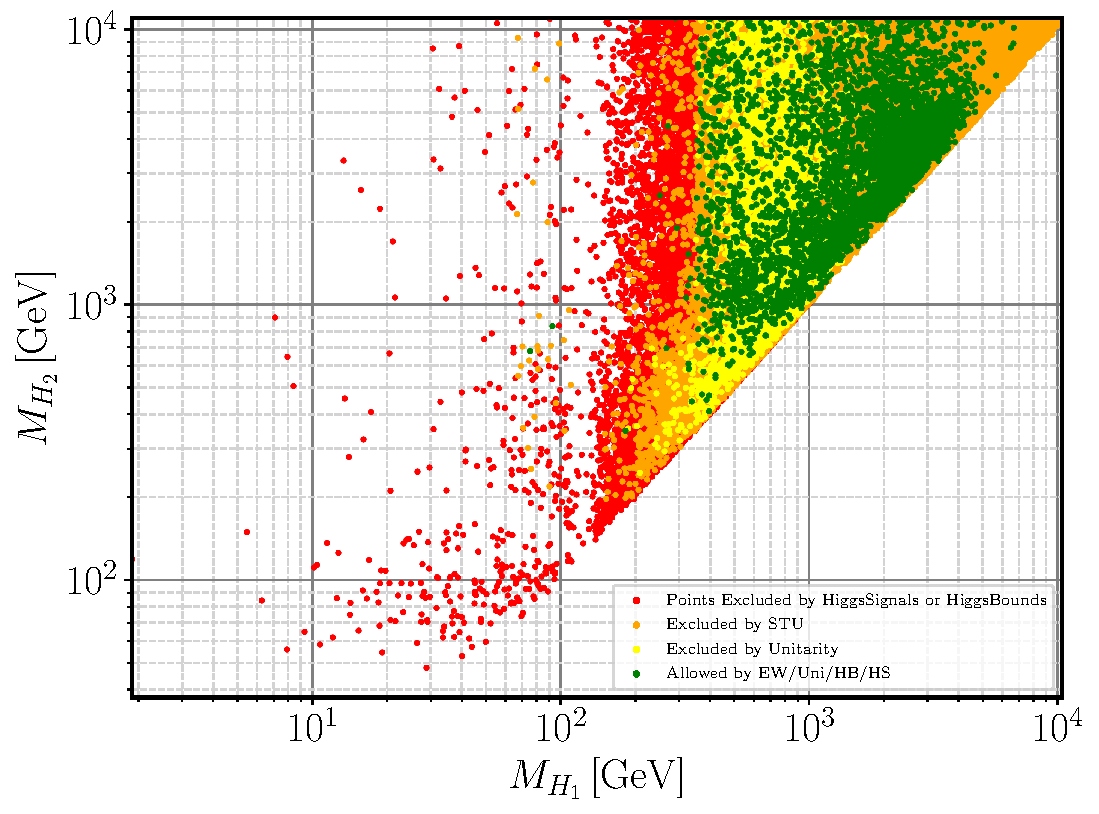
\includegraphics[width=.49\textwidth]{/3HDM/H1_H2.pdf}
	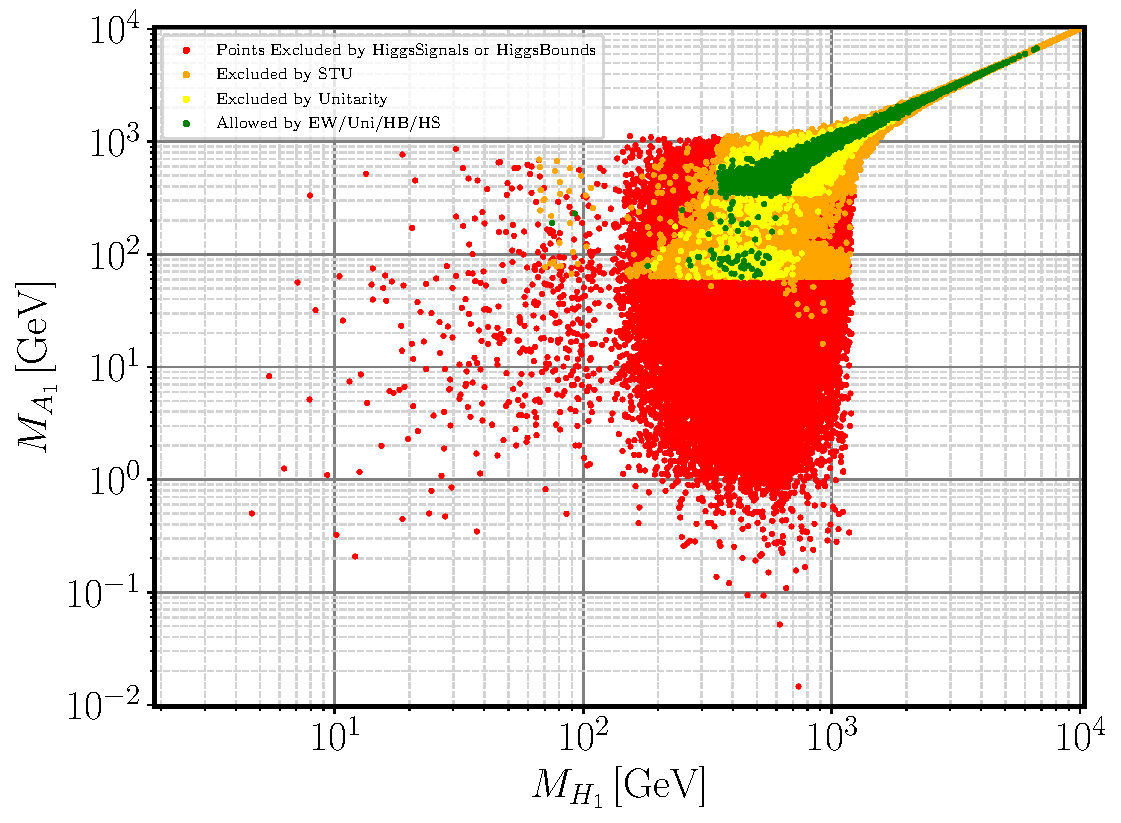
\includegraphics[width=.49\textwidth]{/3HDM/H1_A1.pdf}
\end{figure}	
\begin{figure}[H]\ContinuedFloat
    \centering
	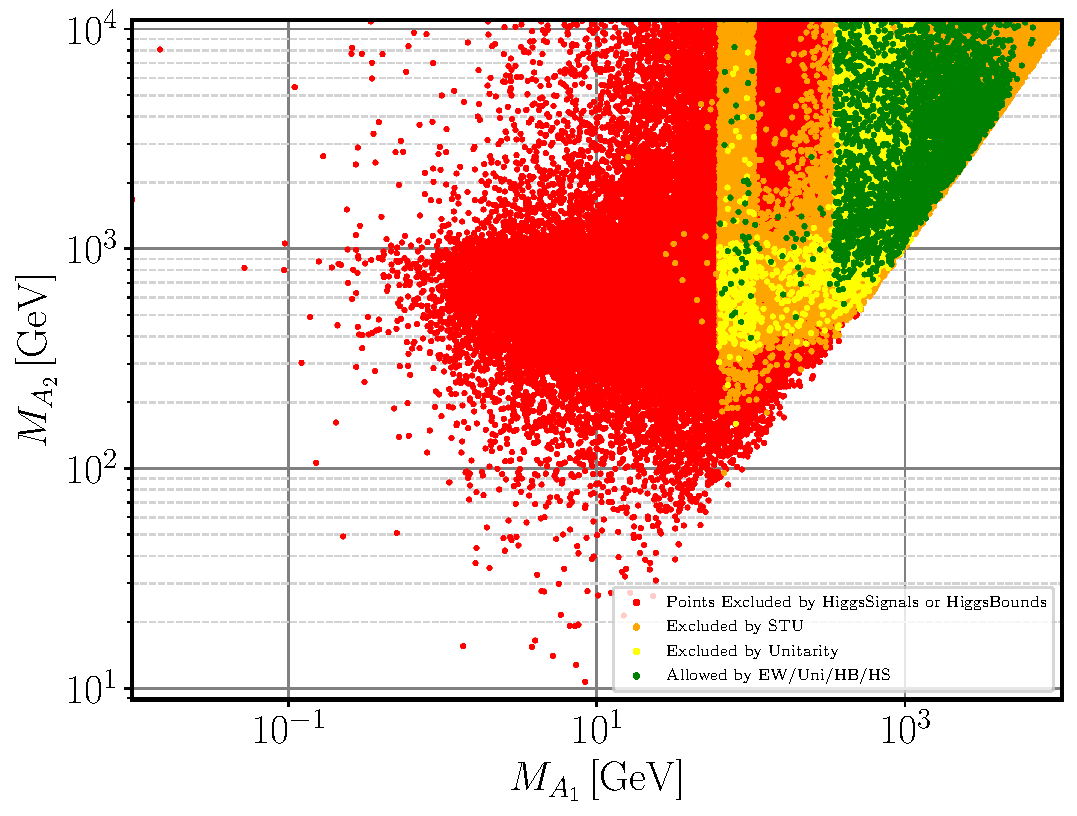
\includegraphics[width=.49\textwidth]{/3HDM/A1_A2.pdf}
	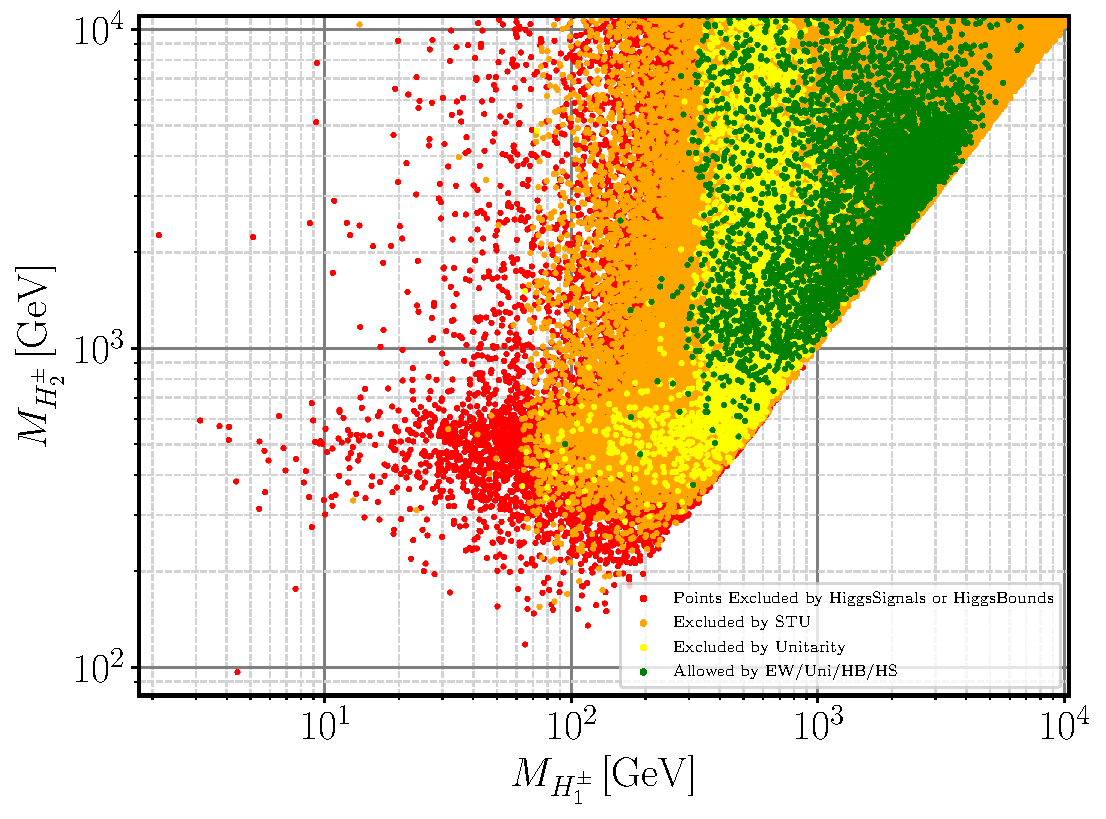
\includegraphics[width=.49\textwidth]{/3HDM/Hc1_Hc2.pdf}
	\caption{Scatter plots of parameter space allowed under several cuts imposed on the BGL-like 3HDM. On the upper right side we have the plot showing the masses of the two heavier CP-even scalars $H_2$ and $H_1$ while in the right we show the relation between the lightest (non SM Higgs) of the CP-even and pseudoscalar particles. As for the bottom plots see the remaining CP-odd scalars and how they are excluded under several cuts. Right we have the pseudoscalar masses $A_1$ and $A_2$ while in the left side we have the CP- odd charged Higgs states $H_1^\pm$ and $H_2^\pm$.	Red points failed HS and HB tests; yellow points violate unitarity constraints; orange points only fail electroweak precision constraints, and green ones satisfy all restrictions.}
	\label{fig:H1_A1_Plots}
\end{figure}	

%One important characteristic of our results worth discussing is the presence of relatively light  scalars. 
%
We can observe that direct searches tightly constrain the pseudoscalar and scalar masses. 
%
These direct search exclusions are directly tied to the red zones where HiggsBounds and HiggsSignals do not allow scalars to exist. 
%
Further examination of these areas shows, firstly the lighter values for the pseudoscalar masses are all excluded by direct Higgs. However there is space for pseudoscalars in case they are "masked" by the observed SM-like Higgs boson signal.  
%
As for all other scalars there does not seem to be a way to reproduce the same effect. 

Furthermore, observing the top right figure in Fig\,\ref{fig:H1_A1_Plots}, direct searches are not responsible for the exclusion of lighter charged Higgs, but our model can not respect STU limits and unitarity constraints for ligther charged Higgs.  

%Next there is a zone within where STU limits are fulfilled at 95 \% C.L. and within that zone we see that only a small region respects unitarity constraints. 
%
We can then argue that our model should predict the existence of masses as low as a few hundred GeVs motivating the continuation of direct searches at the LHC. 
%
The precise values for benchmark points will be presented after the Quark flavour observables are performed. 

%{ \color{red} Ask morais : why do pseudo scalar masses tend to funnel? }  

%We can then argue that our model predicts the existence of masses around (300's GeVs check in detail later) which are in harmony with the SM i.e. are so far compatible with observations. 

A feature of HiggsBounds is it also enables us to see the most stringent channel for a given parameter point. 
%
From this we can see the most stringent channels that constrict our model are di-photon production and gluon fusion into light scalars (Limits taken from Refs. \cite{Aad_2014,CMS-PAS-HIG-14-029,Khachatryan_2015}). 
%
%It could be that by requiring that we have a SM-like Higgs boson, naturally imposes conditions upon the couplings of the heavier (or lighter) CP-even scalar states to the Gauge bosons. This should enable most of the Higgs sector to be within bounds. 
%
%, and seeing that the harshest condition on most scalar sectors is the di-Z production we then have that due to the alignment limit imposed the majority of the scalar sector is allowed. 
%
%We can also see that unless the signal coming from the pseudoscalar masses is masked by the Higgs SM signal or the pseudoscalar is heavy (in the TeV region) that it poses a harsh cut on the parameter space.

%{ \color{red} Why then are the pseudoscalars so constricted. }   

\subsubsection{Flavour Cuts }

% Having shown that there are no instances of heavy fine tuning in our model. 

Let us now look at the QFV observable results, first by constraining all the most stringent QFV to be within 2 $\sigma$ bounds as discussed previously,
%
% Before showing what combined regions we observe stemming from the cuts discussed above when combined with QFV observables, it might be a worth while endevour to see what type of regions we can see with only QFV observables. 
%
%First we show what the fractions of QFV observables show,    
%
%\begin{figure}[H]
%	\centering
%	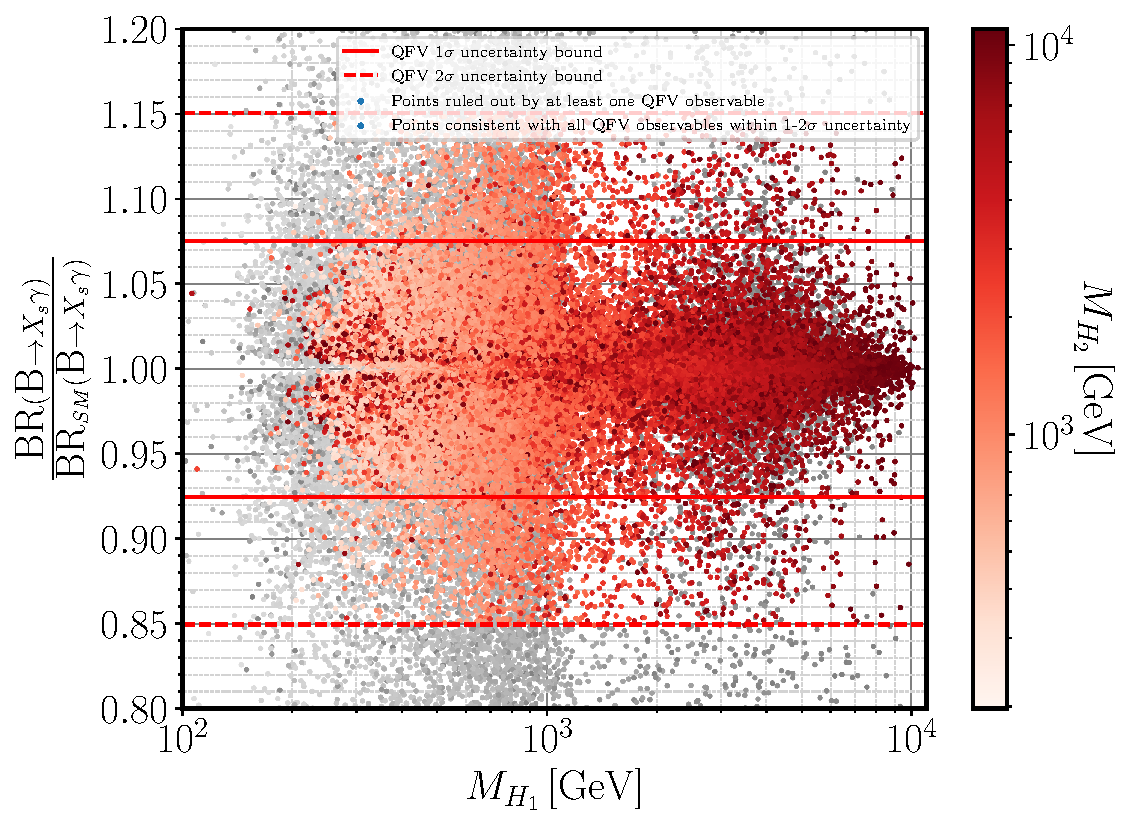
\includegraphics[width=.49\textwidth]{Images/3HDM/Reds/Xsgamma_H1_H2.pdf}
%	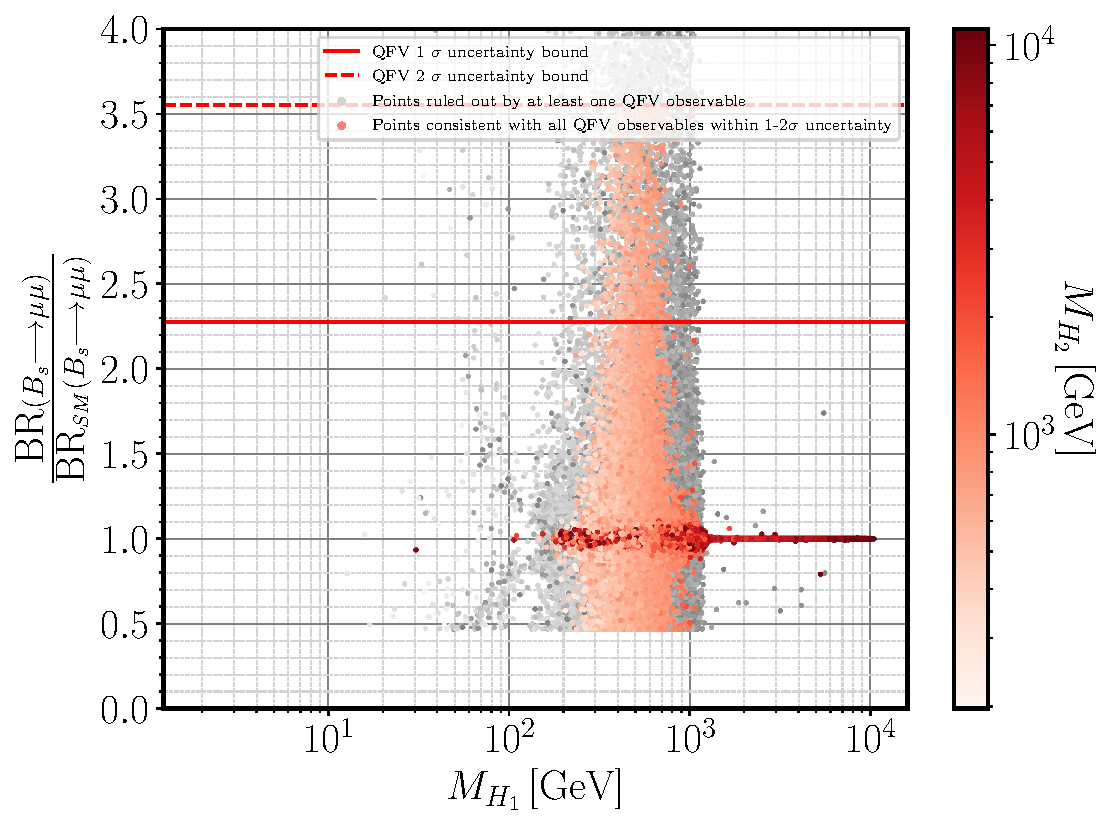
\includegraphics[width=.49\textwidth]{Images/3HDM/Reds/Bsmumu_H1_H2.pdf}
%\end{figure}
%\begin{figure}[H]\ContinuedFloat
%    \centering
%	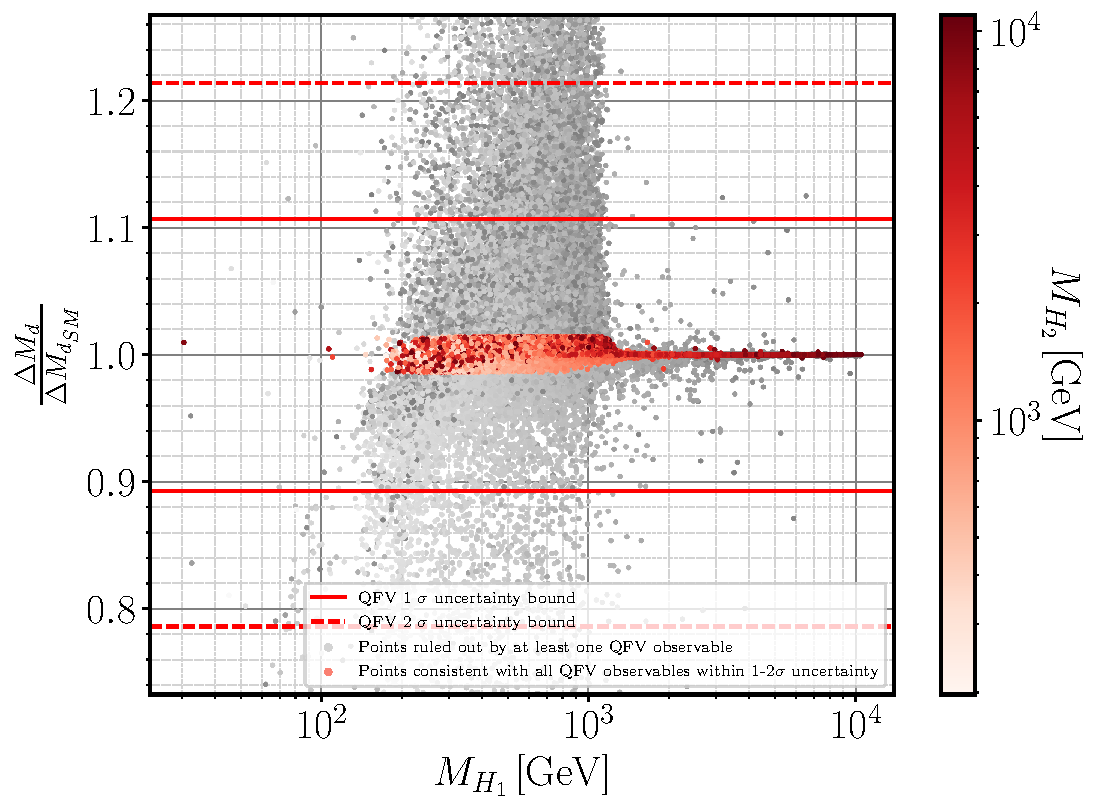
\includegraphics[width=.49\textwidth]{Images/3HDM/Reds/DeltaMd_H1_H2.pdf}
%    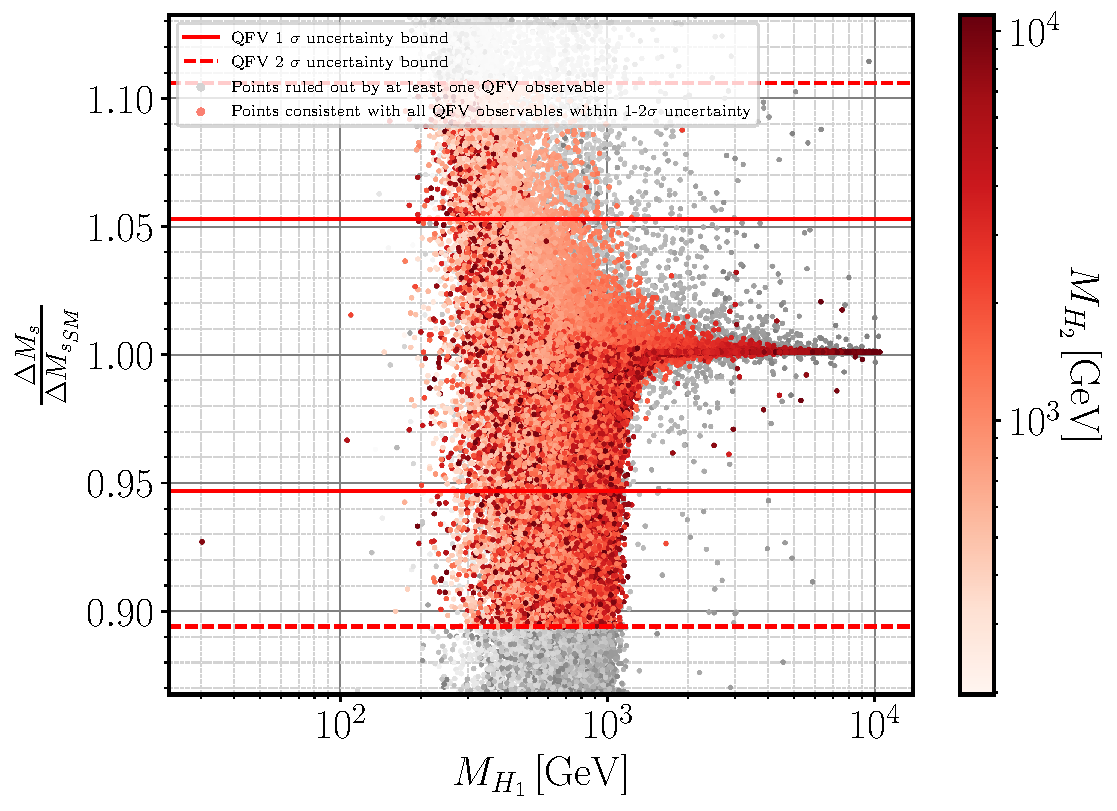
\includegraphics[width=.49\textwidth]{Images/3HDM/Reds/DeltaMs_H1_H2.pdf}
%\end{figure}
%\begin{figure}[H]\ContinuedFloat
%    \centering
%    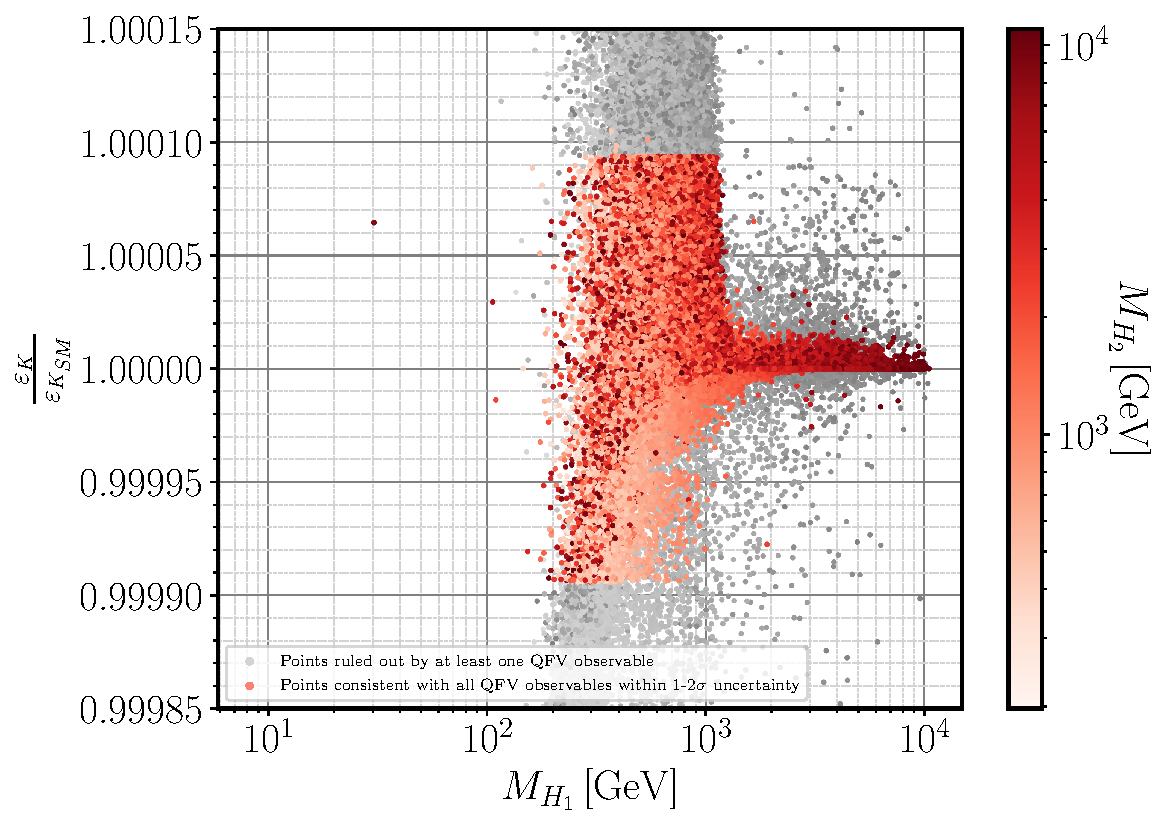
\includegraphics[width=.49\textwidth]{Images/3HDM/Reds/Eps_K_H1_H2_Centered.pdf}
%	\caption{ Scatter plot of the estimated QFV observables normalized to the SM values versus the lightest scalar Higgs. The grey points in all plots represent a point that would be outside the 2 $\sigma$ bound for one of the observables while in a red color scale we see the second CP-even neutral scalar mass for the remaining points. % {\color{blue} Ask, anyone of these are $H^\pm$ only? is it worth swapping H?}  
%	}
%	\label{fig:3HDM_Flavour}
%\end{figure}

\begin{figure}[H]
\centering
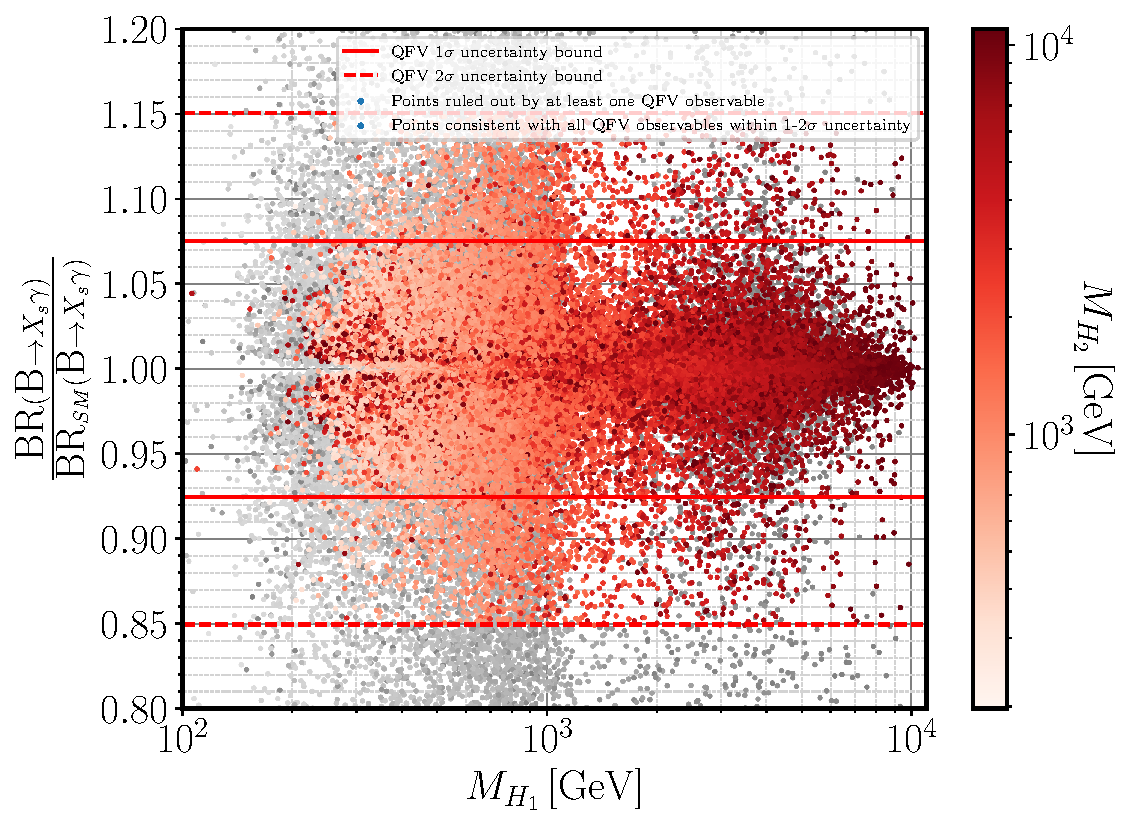
\includegraphics[width=.49\textwidth]{Images/3HDM/Reds/Xsgamma_H1_H2.pdf}
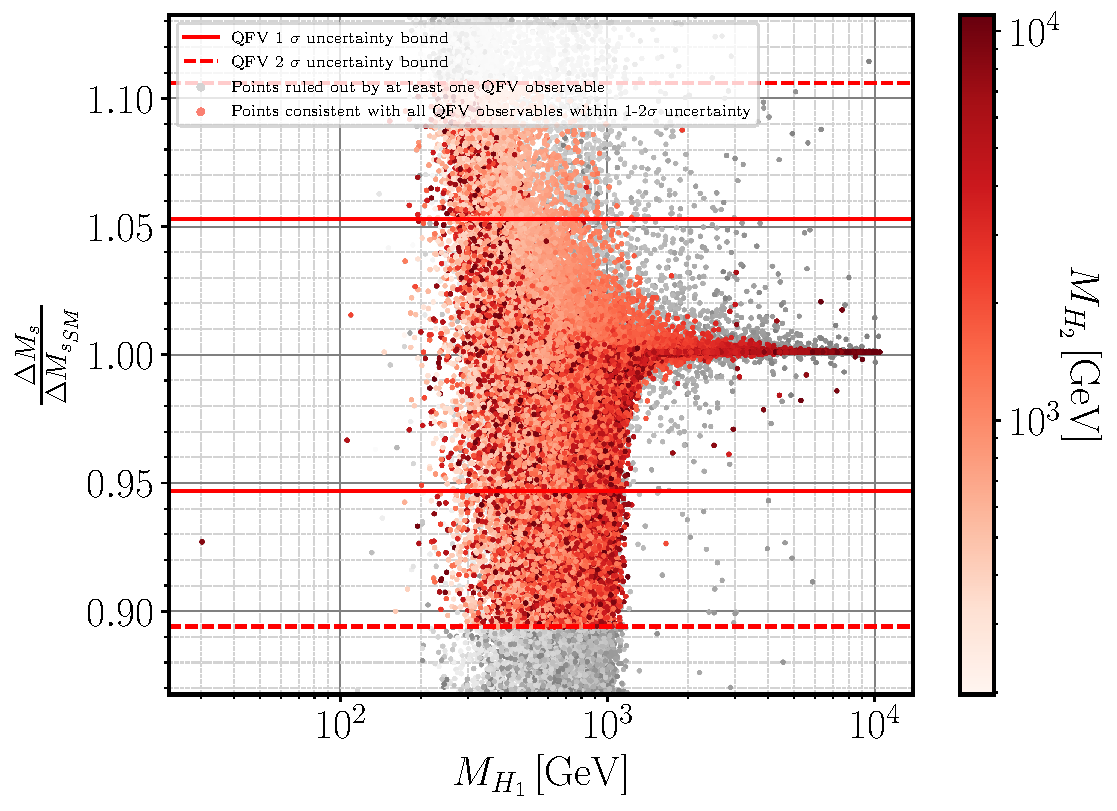
\includegraphics[width=.49\textwidth]{Images/3HDM/Reds/DeltaMs_H1_H2.pdf}
%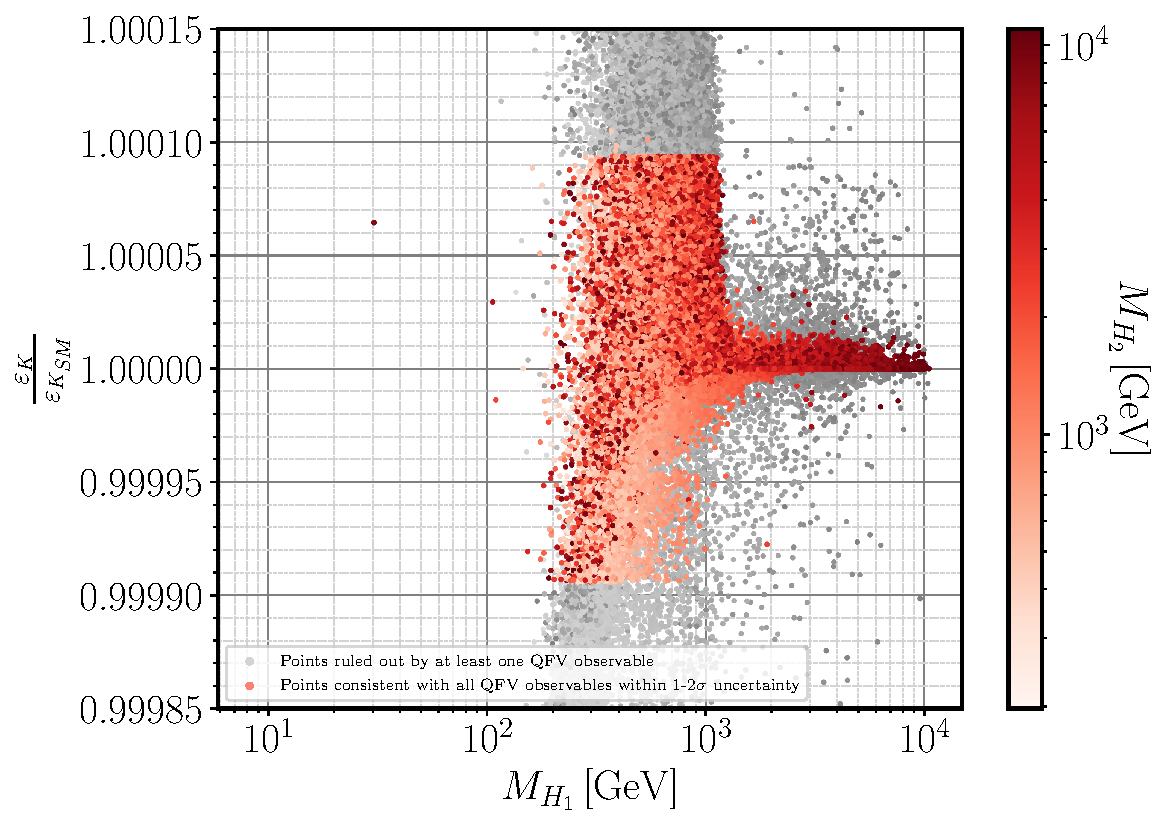
\includegraphics[width=.49\textwidth]{Images/3HDM/Reds/Eps_K_H1_H2_Centered.pdf}
	\caption{ Scatter plot of the estimated QFV observables normalized to the SM values versus the lightest scalar Higgs. The grey points in all plots represent a point that would be outside the 2 $\sigma$ bound for one of the observables while in a red color scale we see the second CP-even neutral scalar mass for the remaining points. % {\color{blue} Ask, anyone of these are $H^\pm$ only? is it worth swapping H?}  
	}
	\label{fig:3HDM_Flavour}
\end{figure}

%The bounds shown in these Figures are seen in, 

%\begin{table}[H]
%\centering
%\begin{tabular}{|l|c|c|c|c|c|c} 
%\hline
%                           & $\dfrac{\textrm{BR} ( \textrm{B} \rightarrow X_s \gamma)}{\textrm{BR}_{SM} ( \textrm{B} \rightarrow X_s \gamma )}$ &  $\dfrac{ \textrm{BR} (B_s  \longrightarrow  \mu  \mu )}{\textrm{BR}_{SM}(B_s  \longrightarrow  \mu  \mu ) }$  
%                           & $\dfrac{\Delta M_d}{\Delta M_{d_{SM}} }$ 
%                           & $\dfrac{\Delta M_s}{\Delta M_{s_{SM}} }$
%                           & $\dfrac{\varepsilon_K}{\varepsilon_{K_{SM}}}$   \\ \hline 
%$1 \sigma$ upper QFV bound &  1.08    &  2.27   &  1.10     &  1.05     &    1.13    \\ \hline 
%$1 \sigma$ lower QFV bound &  0.91    &  0.00   &  0.91     &  0.95     &    0.87    \\ \hline 
%$2 \sigma$ upper QFV bound &  1.15    &  3.55   &  1.21     &  1.10     &    1.27    \\ \hline 
%$2 \sigma$ lower QFV bound &  0.85    &  0.00   &  0.79     &  0.90     &    0.72    \\ \hline  
%\end{tabular}
%\caption{Calculated 1 and 2 $\sigma$ bounds for QFV observables}
%\end{table}

Note the available zone for $\varepsilon_K/\varepsilon_{K_{SM}}$ and some other decays seems quite small, this is due to ${\textrm{BR} ( \textrm{B} \rightarrow X_s \gamma)}/{\textrm{BR}_{SM} ( \textrm{B} \rightarrow X_s \gamma )}$ and ${\Delta M_s}/{\Delta M_{s_{SM}} }$ being very tightly constraint and the most sensitive in our model.

When combined with the EW and scalar analysis these exclusions wield, 

\begin{figure}[H]
	\centering
	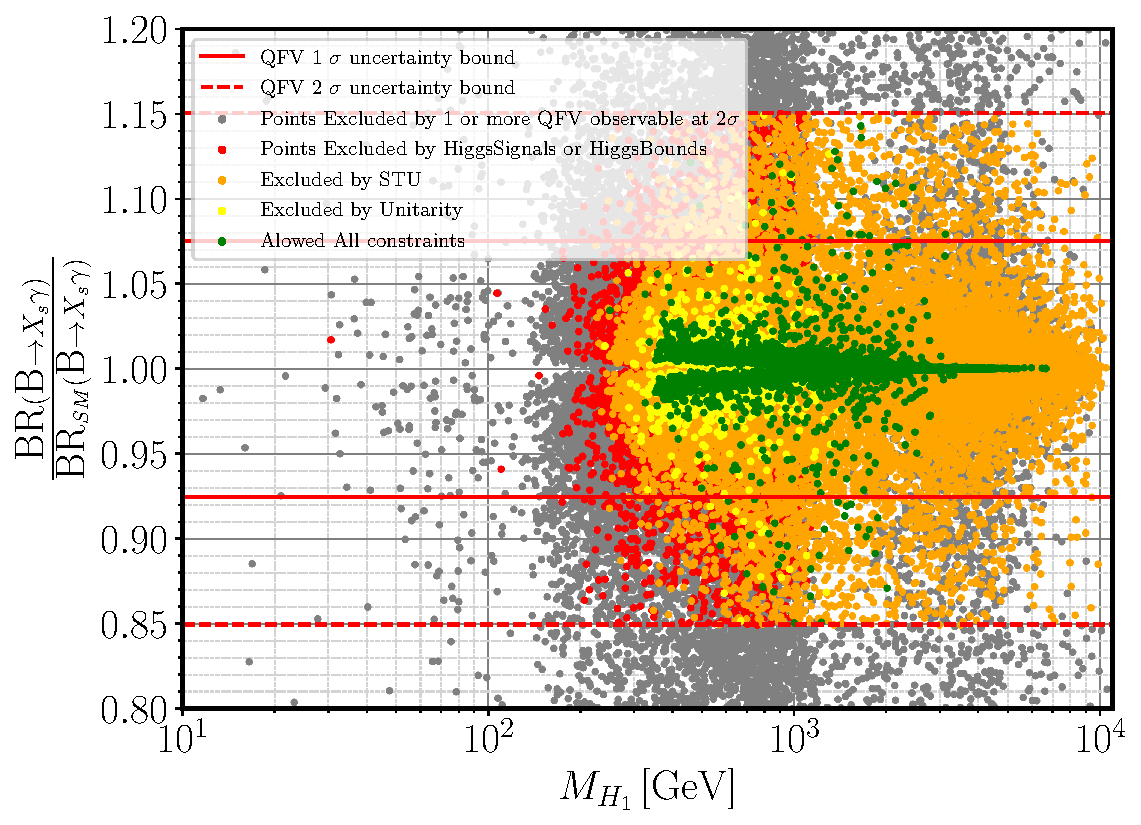
\includegraphics[width=.49\textwidth]{Images/3HDM/PT_Folder/XsGamma_H1.pdf}
	%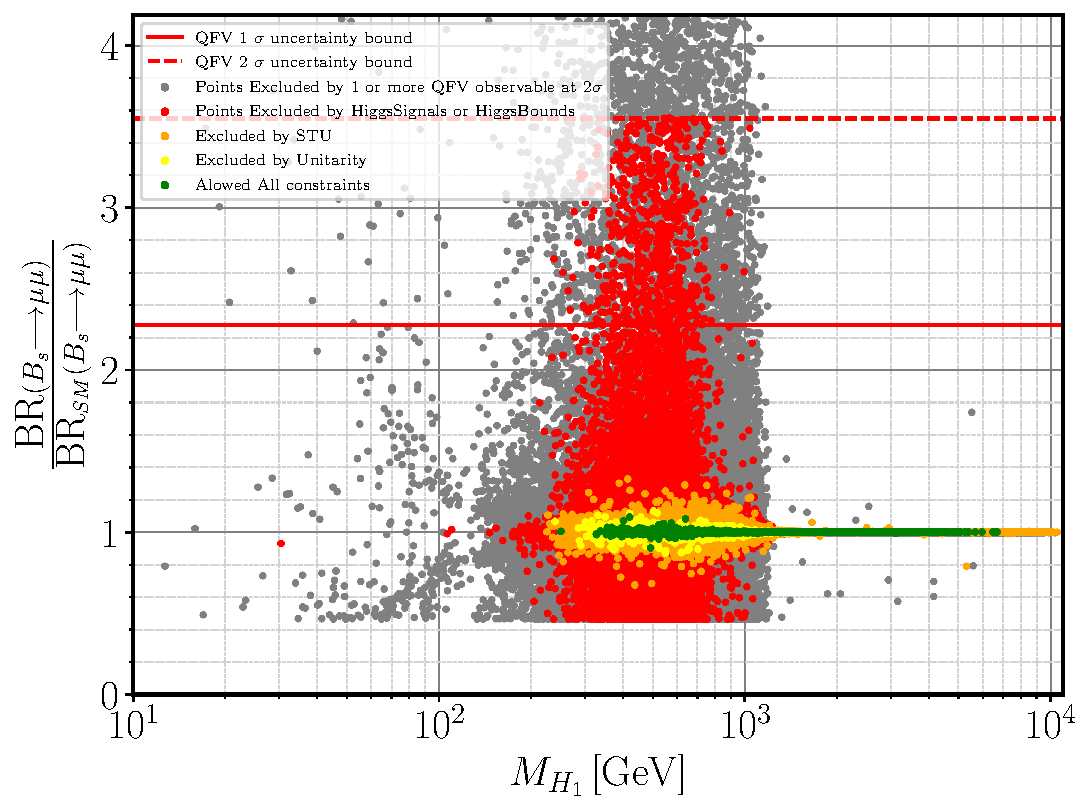
\includegraphics[width=.49\textwidth]{Images/3HDM/PT_Folder/Bsmumu_H1.pdf}
    %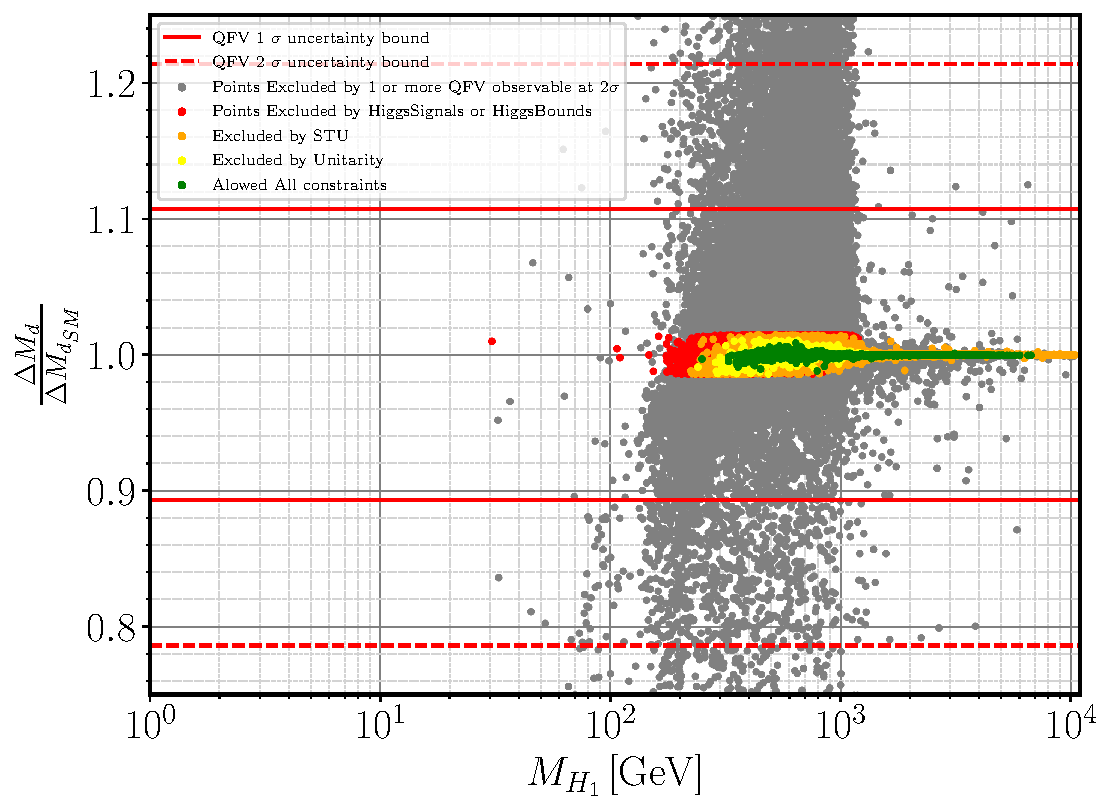
\includegraphics[width=.49\textwidth]{Images/3HDM/PT_Folder/Delta_Md_H1.pdf}
    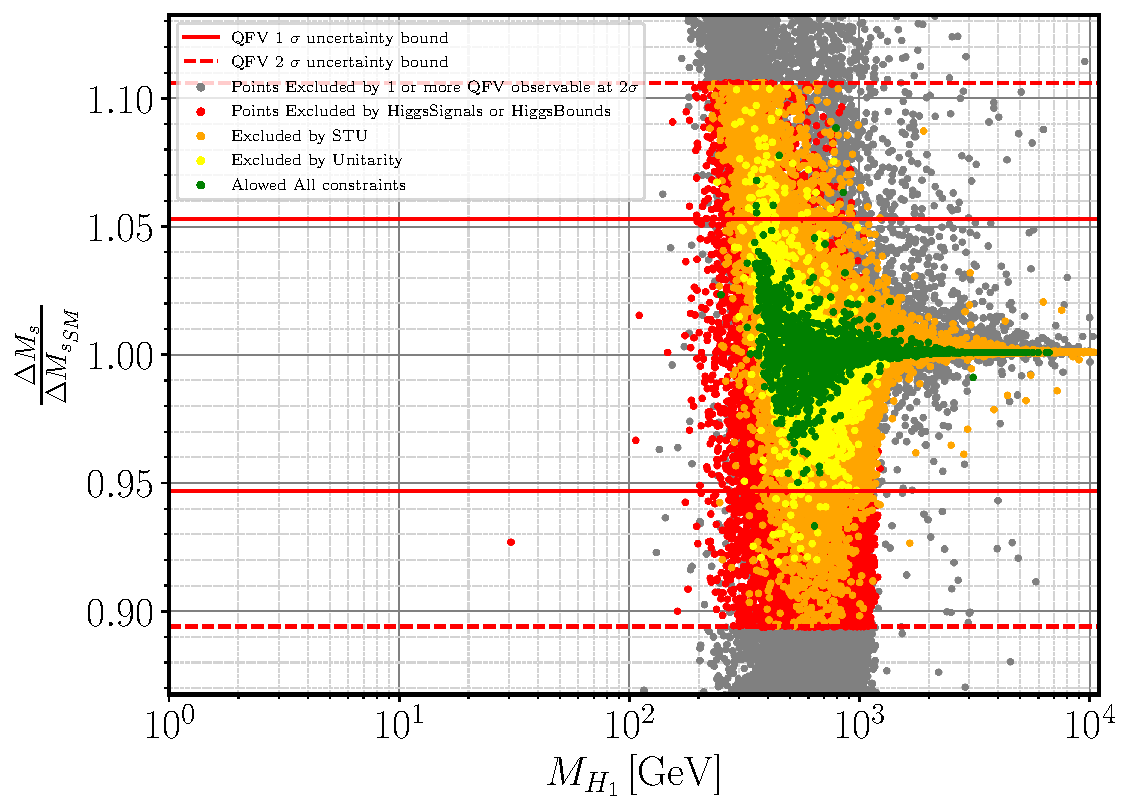
\includegraphics[width=.49\textwidth]{Images/3HDM/PT_Folder/Delta_Ms_H1.pdf}
    %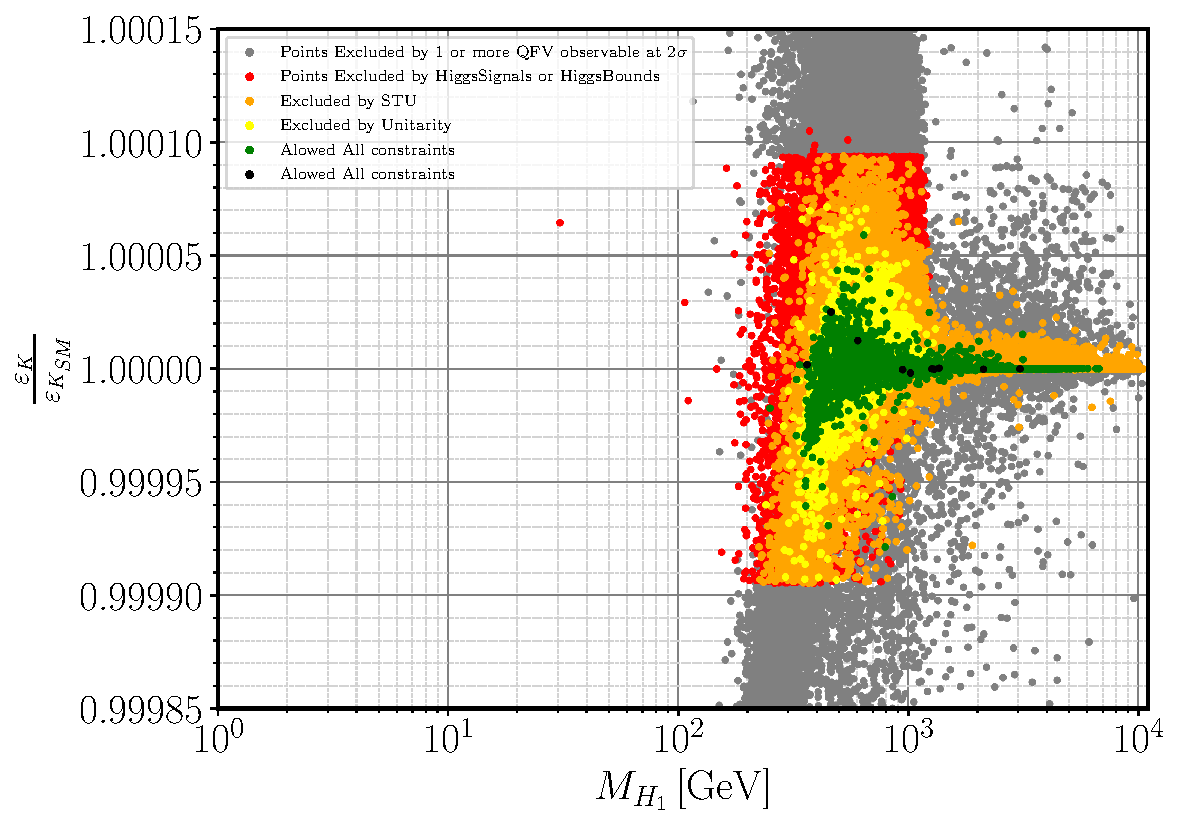
\includegraphics[width=.49\textwidth]{Images/3HDM/PT_Folder/Eps_K_H1_Thighter_Centered.pdf}
    \caption{ Scatter plot of the estimated QFV observables normalized to SM values overlaped with EW and Higgs sector just as in previous figures. } 
	\label{fig:3HDM_Flavour_PT}
\end{figure}	

Here you can clearly see that there is a central region where the points that verify all EW and scalar constraints are all also consistent with QFV observables. 
%
This is a very important conclusion we take from our model. Trough the stabilization of the 3HDM by the flavour symmetry all QFV observables are kept under significant deviation for all the viable mass spectrum.  

We can now extract possible bench mark points, these are written in Tab.\,\ref{Tab:BadTable}.
%
%\begin{table}[H]
%\label{tab:3HDM-Benchmarks-Mass}
%\centering
%\begin{tabular}{l|c|c|c|c|c|c|}
%\cline{2-7}
%                                                  & $H_1$ & $H_2$ & $A_1$ & $A_2$ & $H_1^\pm$ & $H_2^\pm$ \\ \hline
%\multicolumn{1}{|l|}{$\text{Max}_M \ (\text{GeV})$} & 6664  & 10979 & 6683  & 10995 & 6623      & 10989     \\ \hline
%\multicolumn{1}{|l|}{$\text{Min}_M \ (\text{GeV})$}              & 251   & 412   & 87    & 395   & 157       & 374       \\ \hline
%\end{tabular}
%\caption{Possible new discovery points, lightest set of scalars that survive all constraints.}
%\end{table}

%\begin{table}[!htb]
%\centering
%\begin{tabular}{|c|c|c|c|c|c|c|}
%\hline
%                          & $m_{H_1}$ (GeV) & $m_{H_2}$ (Gev) & $m_{A_1}$  (GeV) & $m_{A_2}$  (GeV) & $m_{H^\pm_1}$  (GeV) & $m_{H^\pm_2}$  (GeV) \\ \hline
%Lightest $H_1$            & 251 & 2488 & 247 & 2616 & 157 & 2510    \\ \hline
%Second lightest $H_1$     & 327 & 1528 & 359 & 1616 & 229 & 1561    \\ \hline
%Lightest $A_1$            & 386 & 452  & 87  & 467 & 189  & 466      \\ \hline
%Second lightest $A_1$     & 337 & 446  & 100 & 395 & 311  & 374      \\ \hline
%Lightest $H^\pm_1$        & 251 & 2488 & 247 & 2616 & 157 & 2510   \\ \hline
%Second lightest $H^\pm_1$ & 398 & 1314 & 282 & 1525 & 173 & 1314
%
%      \\ \hline
%\end{tabular}
%\end{table}

%
\begin{table}[H]
\centering
\begin{tabular}{c|c|c|c|c|c|c|}
\cline{2-7} 
                                                          & $m_{H_1}$ & $m_{H_2}$ & $m_{A_1}$ & $m_{A_2}$ & $m_{H^\pm_1}$ & $m_{H^\pm_2}$ \\ \hline
\multicolumn{1}{|c|}{\multirow{2}{*}{Lightest $H_1$}}     & 251 & 2488 & 247 & 2616 & 157 & 2510  \\ \cline{2-7} 
\multicolumn{1}{|c|}{}                                    & 327 & 1528 & 359 & 1616 & 229 & 1561  \\ \hline
\multicolumn{1}{|c|}{\multirow{2}{*}{Lightest $A_1$}}     & 386 & 452  & 87  & 467 & 189  & 466  \\ \cline{2-7} 
\multicolumn{1}{|c|}{}                                    & 337 & 446  & 100 & 395 & 311  & 374  \\ \hline
\multicolumn{1}{|c|}{\multirow{2}{*}{Lightest $H^\pm_1$}} & 251 & 2488 & 247 & 2616 & 157 & 2510 \\ \cline{2-7} 
\multicolumn{1}{|c|}{}                                    & 398 & 1314 & 282 & 1525 & 173 & 1314 \\ \hline
\end{tabular}
\caption{A selection of four benchmark points. All written masses are given in GeV. These correspond to the lightest scalars found that respect all QFV and scalar sector cosntraints.}
\label{Tab:BadTable}
\end{table}

We discussed that some NHDMs use deliberate fine-tuning in their model as to have NP contributions balance out and artificially control flavour changing effects in their models. In this model we do not follow this process, our scans were purely randomly generated.  
%
However, randomness combined with thew large amount of data collected could have found a syncronicity where flavour observables are fine-tunned by accident. 
%
%It was important to verify fine-tunning as our scans randomness could have found a syncronicity where flavour observables are fine-tunned by accident. 

To check if this phenomena was present, all points were recalculated with slight a variation of masses trough a 1\% variation of soft breaking terms, $\mu_{13}$, $\mu_{23}$ and $\mu_{21}$. 
%
Such a mass variation is expected to lead to variation of the flavour channel decay amplitude. 

Trough this exercise we expect to show that a there is no abruptly high variation of masses or QFV observable as to show no fine-tunning is present.
% 
The results can be seen in, 

\begin{figure}[H]
	\centering
	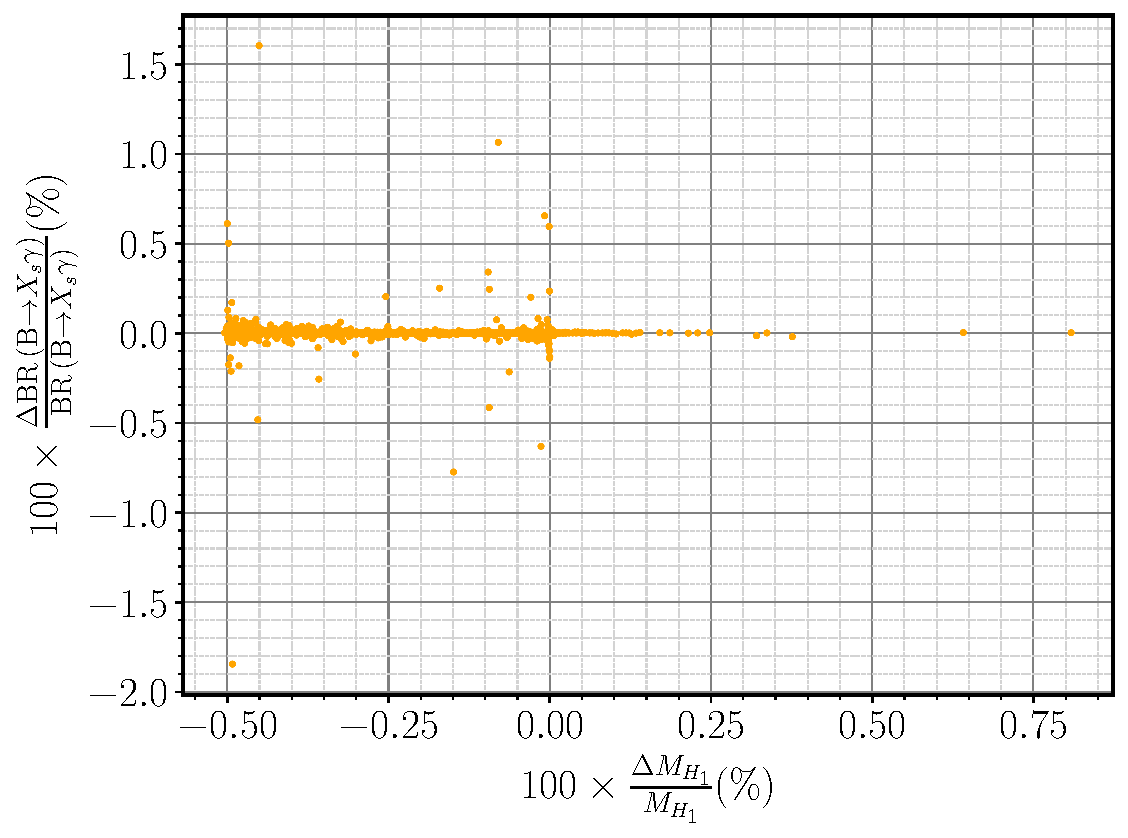
\includegraphics[width=.49\textwidth]{Images/3HDM/Fine_Tuning/Xsgamma_H1.pdf}
	%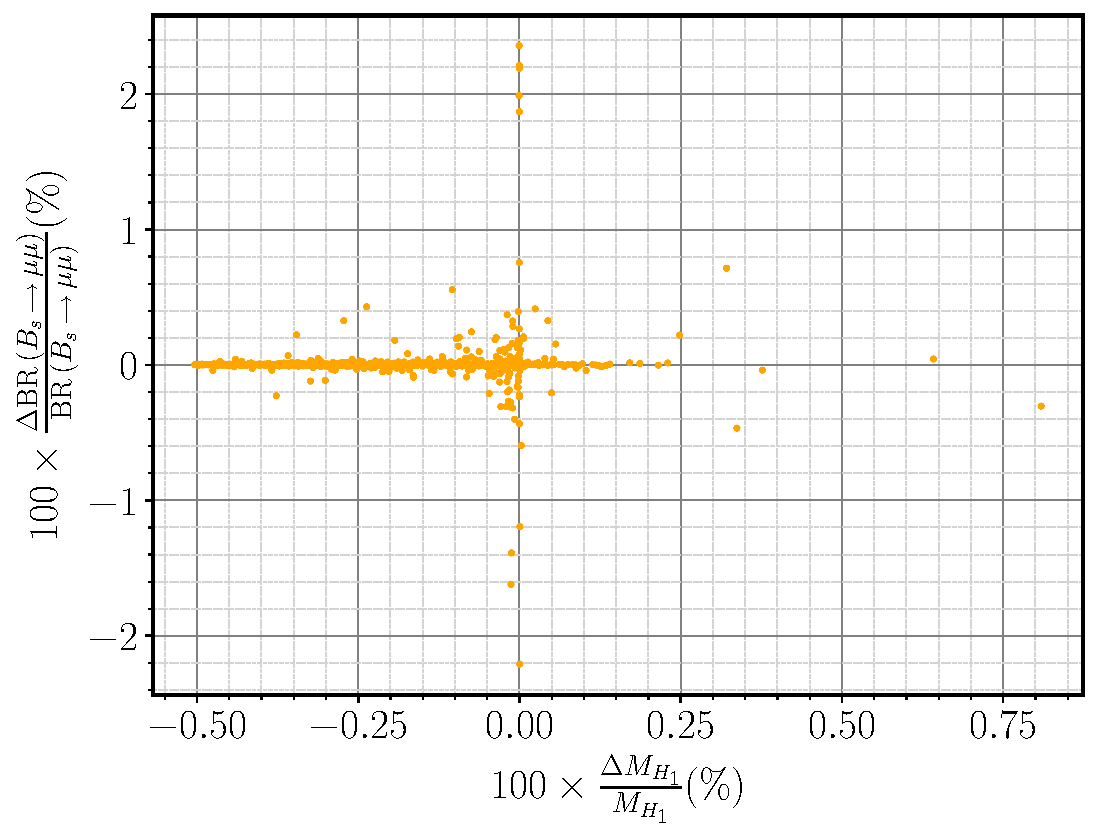
\includegraphics[width=.49\textwidth]{Images/3HDM/Fine_Tuning/Bsmumu_H1.pdf}
	%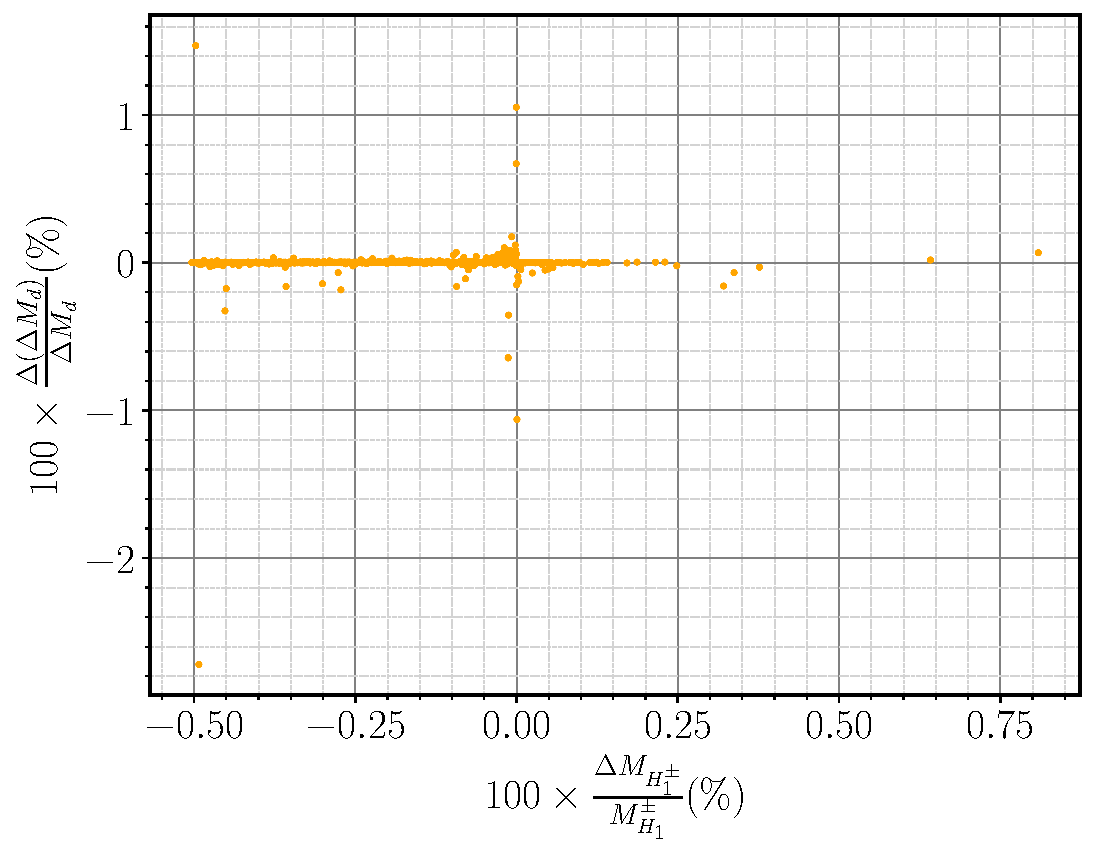
\includegraphics[width=.49\textwidth]{Images/3HDM/Fine_Tuning/DeltaMd_H1.pdf}
    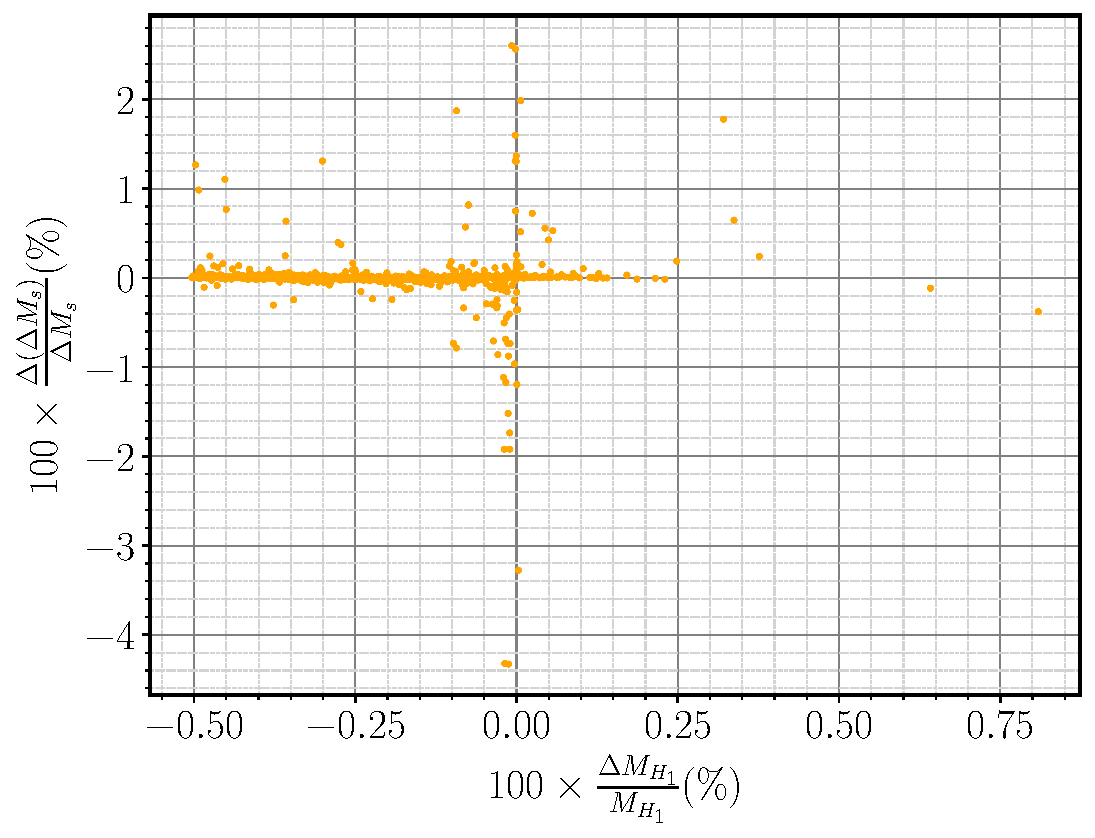
\includegraphics[width=.49\textwidth]{Images/3HDM/Fine_Tuning/DeltaMs_H1.pdf}
    %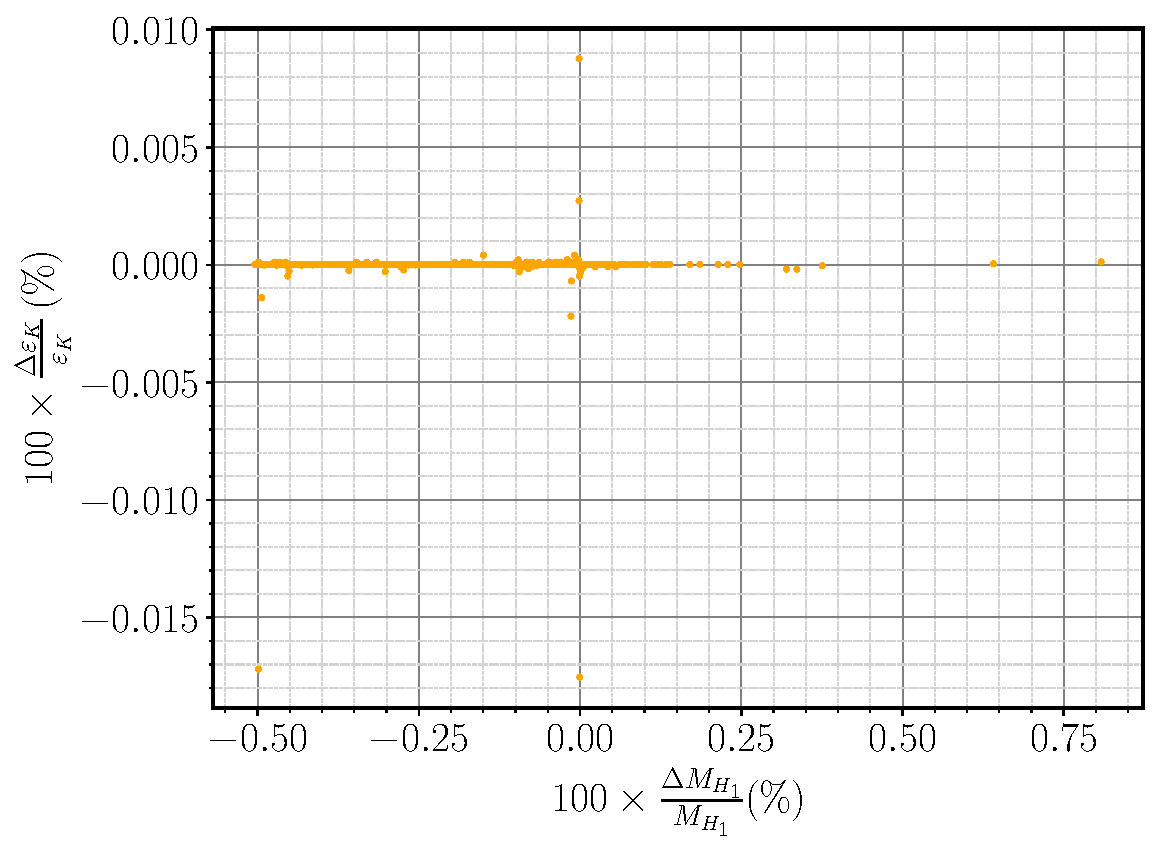
\includegraphics[width=.49\textwidth]{Images/3HDM/Fine_Tuning/eps_K_H1.pdf}
	\caption{Relative mass and QFV observable changes with the increase of 1\% in all softbreaking terms}
	\label{fig:3HDM_Fine_Tunning}
\end{figure}	

Finally a complementary study was also implemented trough Madgraph in this model. 
%
This study served a dual purpose to ensure that proper gluon fusion was being calculated by HiggsBounds and HiggsSignals and to show how close the model was to exclusion. The results are seen in, 
%
\begin{figure}[H]
	\centering
	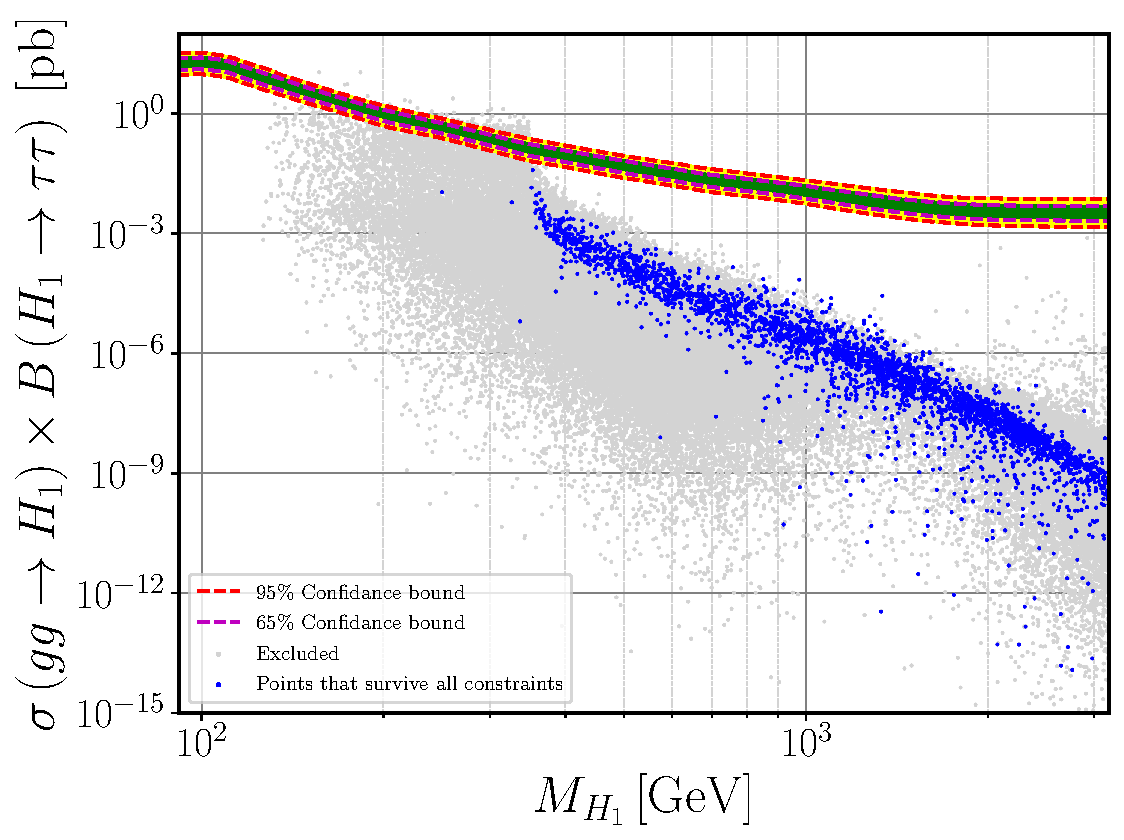
\includegraphics[width=.49\textwidth]{Images/3HDM/Xsec/Xsec_1_Grey_tight.pdf}	%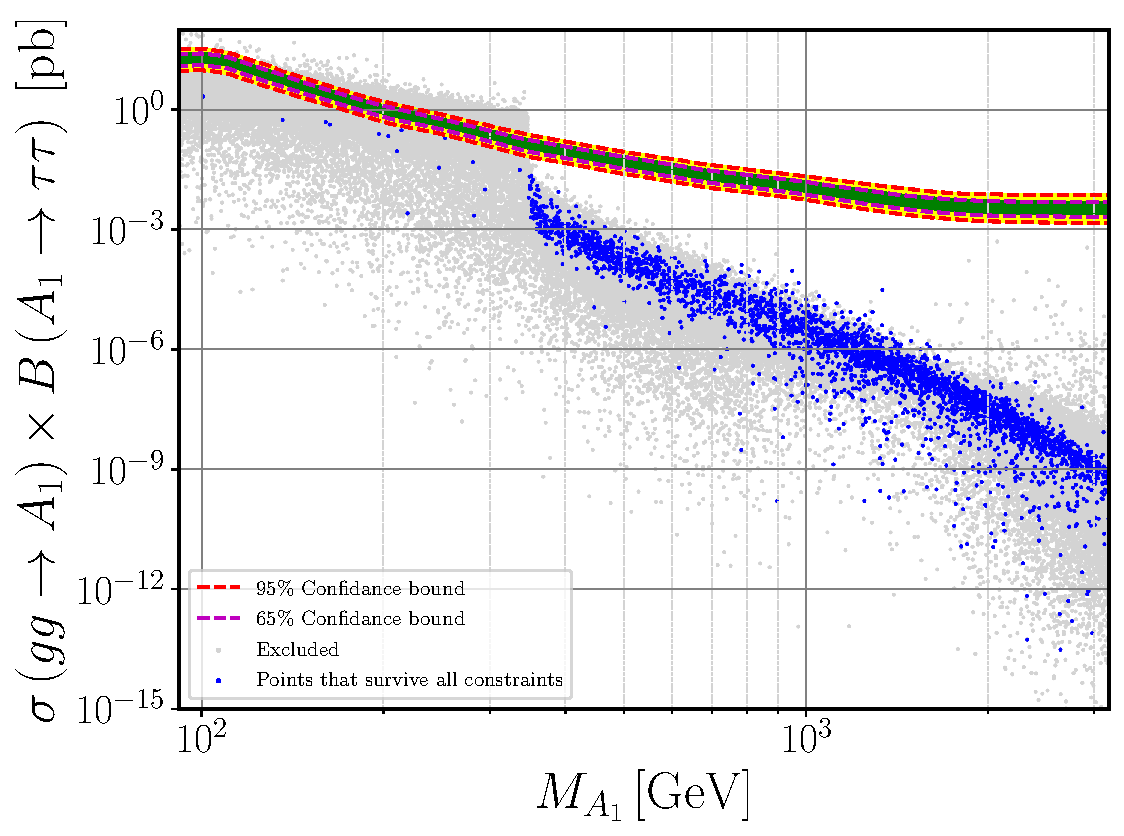
\includegraphics[width=.49\textwidth]{Images/3HDM/Xsec/Xsec_2_Colourful_tight.pdf}
	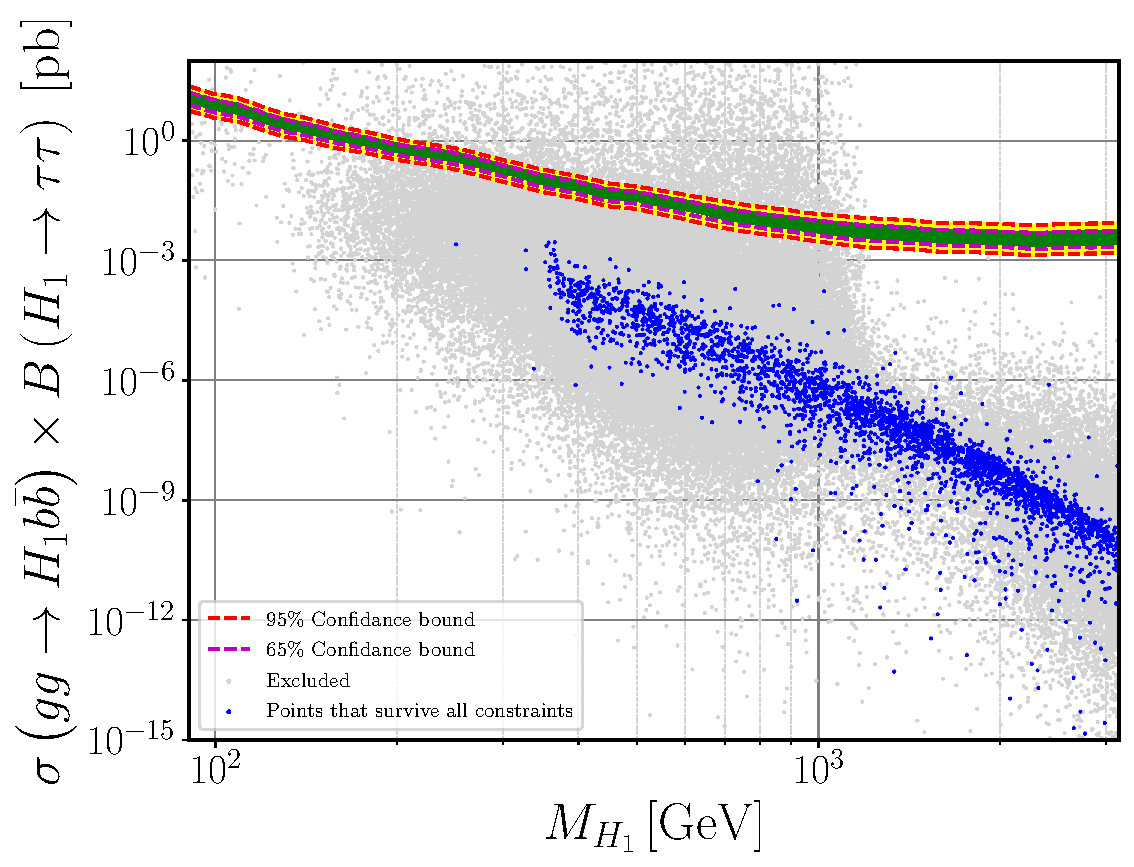
\includegraphics[width=.49\textwidth]{Images/3HDM/Xsec/Xsec_3_Grey_Thight.pdf}
	\caption{}
	\label{}
\end{figure}	
%
With these plots we can see that not only the region is clearly all bellow detection validating HiggsBounds, as we can also see there is space left to be probed at new colider experiments, both near and far from detection. 
%
This means we could be close to a new signature detection at the LHC trough gluon fusion.  

%We can see that there is still plenty of space left to be probed at new versions of the LHC and that the surviving scalars could possibly remain elusive for the considered processes, 

\renewcommand{\cleardoublepage}{}
\renewcommand{\clearpage}{}

\chapter{Conclusions}
\label{ch:Conclusions}

%\section{The B-L-SM Conclusions}
%\label{sec:Conclusions BLSM}

%  
%
%Although this is the basis of the work presented here a effort was made to incorporate new machine learning routines via the initial building of smaller learning sets by conventional methods. 
%
%

To summarize, in this thesis we have performed a detailed phenomenological analysis of the minimal $\U{B-L}$ extension of the Standard Model known as the B-L-SM and the a BGL-like 3HDM with a $\mathrm{U(1)} \times \mathbb{Z}_2$ symmetry. 
%
This phenomenological analysis was produced by a set of tools developed as to be easily adaptable to fit new models. 

Note, although we use conventional means to perform this analysis, some modern studies have incorporated new strategies to scan these complex problems like machine learning. Similar to done by our colleagues in \cite{freitas2020phenomenology}. These new methods promise to greatly increase the efficacy of similar studies. 
%
Unfortunately this wasn't accomplished in this work due to the exceptional setbacks. A feature of this year, that affected partially the quality of the work. 
%
These machine learning routines could reveal much faster


In the B-L-SM (chapter \ref{Chap:B-L-SM_Model}), we have confronted the model with the most recent experimental bounds from the direct $Z^\prime$ boson and next-to-lightest Higgs state searches at the LHC.
%
Simultaneously, we have analysed the prospects of the B-L-SM for a consistent explanation of the observed anomaly in the muon anomalous magnetic moment $(g-2)_{\mu}$. 
%
Done by exploring the B-L-SM potential for the observed $(g-2)_{\mu}$ anomaly in the regions of the model parameter space that are consistent with direct searches and EW precision observables.

As one of the main results of our analysis, we have found phenomenologically consistent parameter space regions that simultaneously fit the exclusion limits from direct $Z^\prime$ searches and can explain the muon $(g-2)_{\mu}$ anomaly. 
%
We have distinguished four benchmark points for future phenomenological exploration at experiments, the first one with the lightest allowed $Z^\prime$ ($m_{Z^\prime}>3.1$ TeV), the second with the lightest additional scalar boson ($m_{h_2}>400$ GeV), and the other two points that reproduce the muon $(g-2)_{\mu}$ anomaly within $1\sigma$ uncertainty range. 
%
Besides, we have studied the correlations of the $Z^\prime$ production cross section times the branching ratio into a pair of light leptons versus the physical parameters of the model.
%
In particular, we have found that the muon $(g-2)_{\mu}$ observable dominated by $Z^\prime$ loop contributions lies within the phenomenologically viable parameter space domain. 
%
For completeness, we have also estimated the dominant contribution from the Barr-Zee type two-loop corrections and found a relatively small effect.

%%%%%% 

As for the 3HDM portion of our work in this these seen in  Chapter\,\ref{ch:3HDM}. 
%
We verified the phenomenological consistency of our model, we identified a region where both flavour and scalar sector physics are within experimental bounds including, like in the B-L-SM, EW precision observables and direct detection bounds.  
%
%We noted that there is a large region of the paramater space that is consistent with flavour QFV observables and where they are not respected. 
%
Narrowing down consistent the parameter space regions that simultaneously fit the exclusion limits from direct scalar searches and flavour constraints. 

For this we determined the most sensitive flavour violation channels, and concluded that the stabilizing flavour symmetry is a mechanism that allows the model to be consist with current flavour observations. 
%
We also propose that further deviations in these flavour observables might be a pathway as to discover Higgs boson (or other exotic particle) mediating these phenomena. 
%
Being that the most appropriate channels to peer into this could be B meson oscillations and B meson decays for this type of 3HDM.

However a key take away from our results we show that the most stringent constraint on the model is not the flavour observables but the Higgs physics limits. 
%
A significant conclusion seeing that new upgrades at the LHCb, Belle and Atlas experiments could mean that despite the flavour sector being constraint the lightest possible Higgs might soon be in the TeV range. 

We recognize these conclusions might not be sufficient to fully examine the model since there might be room for a wider paramater space if exact alignment is not performed or if loop order effects are allowed.

In our study of the 3HDM we have highlighted six benchmark points to illustrate how low masses are still within the range of future colider experiments.

% {\color{blue} I am unsure what to add } 

%We have distinguished four benchmark points for future phenomenological exploration at experiments, the first one with the lightest allowed $Z^\prime$ ($m_{Z^\prime}>3.1$ TeV), the second with the lightest additional scalar boson ($m_{h_2}>400$ GeV), and the other two points that reproduce the muon $(g-2)_{\mu}$ anomaly within $1\sigma$ uncertainty range. 

%Especially if this mixing comes from light scalars. 
%
%Note that we found that there are exotic scalars with very light masses that sucessful pass all constraints. 
% 
%This study might pave the way for continued work in direct scalar searches. 

%T some of the allowed exotic scalars are found to be light indicating that the model succeeds in confronting flavour data even in the presence of scalars as lightas 300 GeV. Hence, the studied 3HDM opens the door to direct searches for non-SM scalarsat future runs of the LHC.

%As for the 3HDM presented in Chapter\,\ref{ch:3HDM}. 
%
%Our numerical analysis show that a 3HDM Model when stabilized trough a flavour symmetry that is softly broken can provide a way to suppress the appearance of tree-level FCNCs. 
%
%Although these FCNCs mediated by the scalar fields have NP contributions that can be sizable, but are not when scalar scattering is considered. 
%
%We also discuss that there are stronger constraints on the model coming from it's enlarged scalar sector.
%

%\section{ Future Work}


\begin{comment} 
\begin{appendices}


\chapter{The loop integral \texorpdfstring{$\ro{T}_7(x,y,x)$}{} }
\label{app:T7}

In Appendix B of Ref.~\cite{Feng:2009gn}, the exact integral equations for $\ro{T}_7\left(x,y,z\right)$ are provided. 
In our analysis we consider the limit where $x \gg y = z$, with $x = m_{Z^\prime}^2$ and $y = z = m_t^2$, 
where Eq.~\eqref{eq:T7} provides a good approximation up to a truncation error. Here, we show the main steps 
in determining Eq.~\eqref{eq:T7}. The exact form of the loop integral reads as
\begin{equation}
\begin{aligned}
    \ro{T}_7\left(x,y,y\right) =& -\dfrac{1}{x^2} \varphi_0\left(y,y\right) + 2 y \dfrac{\del^3 \Phi(x,y,y)}{\del x \del y^2} + \dfrac{\del^2 \Phi(x,y,y)}{\del x^2} + x \dfrac{\del^3 \Phi(x,y,y)}{\del x^2 \del y} \\
    & + \dfrac{\Phi(x,y,y)}{x^2}
    -\dfrac{1}{x} \dfrac{\del \Phi(x,y,y)}{\del x}
    + \dfrac{\del^2 \Phi(x,y,y)}{\del x \del y} \,,
\end{aligned}    
\label{eq:T7-Integrals}
\end{equation}
with $\varphi_0 (x,y)$ and $\Phi(x,y,z)$ defined in Ref.~\cite{Feng:2009gn}. Let us now expand 
each of the terms for $x \ll y$. While the first term is exact and has the form
\begin{equation}
    -\dfrac{1}{x^2} \varphi_0\left(y,y\right) = -2 \dfrac{y}{x^2} \log^2 y \,,
    \label{eq:expand1}
\end{equation}
the second can be approximated to
\begin{equation}
    2 y \dfrac{\del^3 \Phi(x,y,y)}{\del x \del y^2} \simeq \xi \dfrac{24}{x} = \dfrac{8}{x} ~\textrm{for}~ \xi = \dfrac{1}{3}\,.
    \label{eq:expand2}
\end{equation}
In Eq.~\eqref{eq:expand2}, the $\xi = \tfrac{1}{3}$ factor was introduced in order to compensate for a truncation error. This was obtained by comparing the numerical values of the exact expression and our approximation. The third term can be simplified to
\begin{equation}
    \dfrac{\del^2 \Phi(x,y,y)}{\del x^2} \simeq \dfrac{2}{x} \left( \log y - \log \dfrac{y}{x} \right) + \dfrac{2}{x} \,,
    \label{eq:expand3}
\end{equation}
and the fourth to
\begin{equation}
    x \dfrac{\del^3 \Phi(x,y,y)}{\del x^2 \del y} \simeq -\dfrac{4}{x}\left(\log \dfrac{y}{x} + 1 \right)\,.
    \label{eq:expand4}
\end{equation}
The fifth and the seventh terms read
\begin{equation}
    \dfrac{\Phi(x,y,y)}{x^2}
    -\dfrac{1}{x} \dfrac{\del \Phi(x,y,y)}{\del x} \simeq \dfrac{2}{x} \log \dfrac{1}{x} \,,
    \label{eq:expand5}
\end{equation}
and finally, the sixth terms can be expanded as
\begin{equation}
    \dfrac{\del^2 \Phi(x,y,y)}{\del x \del y} \simeq \dfrac{4}{x}\left(\log \dfrac{y}{x} -1\right)\,.
    \label{eq:expand6}
\end{equation}
Noting that Eq.~\eqref{eq:expand1} is of the order $\tfrac{1}{x^2}$, putting together Eqs.~\eqref{eq:T7-Integrals}, \eqref{eq:expand2}, \eqref{eq:expand3}, \eqref{eq:expand4}, \eqref{eq:expand5}, and \eqref{eq:expand6} we get for the leading $\tfrac{1}{x}$ contributions the following:
\begin{equation}
    \begin{aligned}
    \ro{T}_7\left(x,y,y\right) \simeq& \overbrace{\dfrac{2}{x} \( \log y - \log \dfrac{y}{x} \) + \dfrac{2}{x} \log \dfrac{1}{x}}^{0} \overbrace{-\dfrac{4}{x}\(\log \dfrac{y}{x} + 1 \) +
    \dfrac{4}{x}\(\log \dfrac{y}{x} -1\)}^{-\tfrac{8}{x}} + \dfrac{8}{x} + \dfrac{2}{x} \simeq \dfrac{2}{x}\,.
    \end{aligned}
    \label{eq:T7-expanded}
\end{equation}
\end{appendices}
\end{comment} 
%\newpage

\bibliographystyle{plain}
\bibliography{bib.bib}

\end{document}
